%% Copernicus Publications Manuscript Preparation Template for LaTeX Submissions
%% ---------------------------------
%% This template should be used for copernicus.cls
%% The class file and some style files are bundled in the Copernicus Latex Package, which can be downloaded from the different journal webpages.
%% For further assistance please contact Copernicus Publications at: production@copernicus.org
%% https://publications.copernicus.org/for_authors/manuscript_preparation.html


%% Please use the following documentclass and journal abbreviations for preprints and final revised papers.

%% 2-column papers and preprints
\documentclass[bg, manuscript]{copernicus}



%% Journal abbreviations (please use the same for preprints and final revised papers)


% Advances in Geosciences (adgeo)
% Advances in Radio Science (ars)
% Advances in Science and Research (asr)
% Advances in Statistical Climatology, Meteorology and Oceanography (ascmo)
% Annales Geophysicae (angeo)
% Archives Animal Breeding (aab)
% Atmospheric Chemistry and Physics (acp)
% Atmospheric Measurement Techniques (amt)
% Biogeosciences (bg)
% Climate of the Past (cp)
% DEUQUA Special Publications (deuquasp)
% Drinking Water Engineering and Science (dwes)
% Earth Surface Dynamics (esurf)
% Earth System Dynamics (esd)
% Earth System Science Data (essd)
% E&G Quaternary Science Journal (egqsj)
% EGUsphere (egusphere) | This is only for EGUsphere preprints submitted without relation to an EGU journal.
% European Journal of Mineralogy (ejm)
% Fossil Record (fr)
% Geochronology (gchron)
% Geographica Helvetica (gh)
% Geoscience Communication (gc)
% Geoscientific Instrumentation, Methods and Data Systems (gi)
% Geoscientific Model Development (gmd)
% History of Geo- and Space Sciences (hgss)
% Hydrology and Earth System Sciences (hess)
% Journal of Bone and Joint Infection (jbji)
% Journal of Micropalaeontology (jm)
% Journal of Sensors and Sensor Systems (jsss)
% Magnetic Resonance (mr)
% Mechanical Sciences (ms)
% Natural Hazards and Earth System Sciences (nhess)
% Nonlinear Processes in Geophysics (npg)
% Ocean Science (os)
% Polarforschung - Journal of the German Society for Polar Research (polf)
% Primate Biology (pb)
% Proceedings of the International Association of Hydrological Sciences (piahs)
% Safety of Nuclear Waste Disposal (sand)
% Scientific Drilling (sd)
% SOIL (soil)
% Solid Earth (se)
% The Cryosphere (tc)
% Weather and Climate Dynamics (wcd)
% Web Ecology (we)
% Wind Energy Science (wes)


%% \usepackage commands included in the copernicus.cls:
%\usepackage[german, english]{babel}
%\usepackage{tabularx}
%\usepackage{cancel}
%\usepackage{multirow}
%\usepackage{supertabular}
%\usepackage{algorithmic}
%\usepackage{algorithm}
%\usepackage{amsthm}
%\usepackage{float}
%\usepackage{subfig}
%\usepackage{rotating}


%\usepackage[nomarkers,figuresonly]{endfloat}
\graphicspath{{pictures/}}
%\graphicspath{{figures/}}

\begin{document}

\title{Parameterization of the responses of subarctic European vegetation to key environmental variables for ozone risk assessment}


% \Author[affil]{given_name}{surname}

\Author[1,4]{Stefanie}{Falk}
\Author[2]{Ane V.}{Vollsnes}
\Author[2]{Aud B.}{Eriksen}
\Author[3]{Lisa}{Emberson}
\Author[3]{Connie}{O'Neill}
\Author[1]{Frode}{Stordal}
\Author[1]{Terje}{Koren Berntsen}

\affil[1]{Department of Geosciences, University of Oslo, Oslo, Norway}
\affil[2]{Department of Biosciences, University of Oslo, Oslo, Norway}
\affil[3]{Department of Environment and Geography, University of York, UK}
\affil[4]{Department of Geography, Ludwig Maximilian University of Munich, Munich, Germany}

%% The [] brackets identify the author with the corresponding affiliation. 1, 2, 3, etc. should be inserted.

%% If an author is deceased, please mark the respective author name(s) with a dagger, e.g. "\Author[2,$\dag$]{Anton}{Smith}", and add a further "\affil[$\dag$]{deceased, 1 July 2019}".

%% If authors contributed equally, please mark the respective author names with an asterisk, e.g. "\Author[2,*]{Anton}{Smith}" and "\Author[3,*]{Bradley}{Miller}" and add a further affiliation: "\affil[*]{These authors contributed equally to this work.}".


\correspondence{Stefanie Falk (stefanie.falk@lmu.de)}

\runningtitle{Response of subarctic European vegetation to key environmental variables}

\runningauthor{Falk et al.}





\received{}
\pubdiscuss{} %% only important for two-stage journals
\revised{}
\accepted{}
\published{}

%% These dates will be inserted by Copernicus Publications during the typesetting process.


\firstpage{1}

\maketitle


\begin{abstract}
  The unique vegetation of the subarctic region acclimatized to extremes of cold and midnight sun are likely to be at threat from the combined impacts of climate change and increasing ozone concentrations \chem{[O_3]}. To date, only a few studies assessed the response of subarctic vegetation to variations in climate and air pollution. This study looks to fill this knowledge gap by examining the uncertainty in risk assessments that are using Boreal paramterizations. With no parameterization of stomatal response of subarctic vegetation available, we propose an adjustment of existing Boreal parameterizations based on local climate condition. To this end, we vary temperature response functions according to the climatological temperature distribution within the growing season at our site. Thus, we refer to our approach as localization of stomatal response functions. With these, we apply the integrated flux-metric Phytotoxic Ozone Dose (POD) to determine ozone risk and damage to vegetation as a function of \chem{[O_3]}, key environmental variables, and species-specific physiology. In addition, we evaluate the extent to which two recent years (2018 and 2019) deviate from climatic and \chem{[O_3]} norms and find that 2018 was an anomalously warm and less cloudy year, particularly in spring and early summer. Higher than average \chem{[O_3]} was observed in April/May while frequent episodes of ozone volume mixing ratios (VMRs) exceeding $40\,\unit{ppb}$ occurred in June--August. These episodes are in part attributable to forest fires in the Northern Hemisphere and warmer and sunnier conditions. In contrast, 2019 was an average year. Our modeling study suggests that using standard Boreal parameterizations in assessments likely leads to underestimating the risk of ozone damage in this region for some species. We find that localized parameterizations for subarctic vegetation result in an ozone-induced biomass loss of $2.5$ to $17.4\,\unit{\%}$. For some species, this loss is up to $55\,\unit{\%}$ larger than projected from Boreal parameterizations used in general assessments. Efforts should be targeted towards accurately defining subarctic vegetations' physiological response to essential climate variables.
\end{abstract}

\newpage

%\copyrightstatement{TEXT}  %% This section is optional and can be used for copyright transfers.

\introduction  %% \introduction[modified heading if necessary]
\label{sec:intro}

Ground-level ozone (\chem{O_3}) is a highly toxic pollutant known to cause damage to a variety of ecosystems around the World \citep{PT:Emberson2020}. Ozone causes reduced photosynthesis, visible foliar injury, early senescence, and programmed cell death of plants \citep{PCE:Kangasjarvi2005}. Hence affecting the global carbon cycle \citep{BGS:Lombardozzi2013} and crop yields. Annual global yield losses of four major crops (wheat, rice, maize, and soybean) of $3-15\,\unit{\%}$ have been reported \citep{PJ:Ainsworth2017} and a suggested loss in primary production in forestry of $7\,\unit{\%}$ \citep{GCB:Wittig2009,EP:Matyssek2012} has been attributed to ozone. Even though long-term (pre-1950) observations of ground-level ozone concentrations are scarce; evidence from trend analysis of those few sites suggests that since the industrial revolution, background concentrations in the northern hemisphere have at least doubled and continued to increase \citep{IPCC2013} until recently. Recent trend analyses for Europe indicate that a maximum was reached in 2007 \citep{AE:Derwent2018}, after which tropospheric background ozone started to level off or even decline \citep{ESA:Cooper2014, ACP:Wespes2018,ESA:Gaudel2018}. This can be attributed to a successful implementation of air quality regulations coupled with economic restructuring, reducing the number of episodes of peak concentrations especially in summertime \citep[e.g.,][]{ESA:Fleming2018, ESA:Mills2018}. However, changes in environmental conditions associated with climate change, such as an increase in the frequency of heatwaves, could negate the effectiveness of emission reductions concerning ozone impacts and air quality \citep{NCC:Lin2020}. Tropospheric background ozone concentrations derived from satellite instruments range between $50-65\,\unit{ppb}$ over Fennoscandia but strongly depend on season \citep{ESA:Cooper2014}.

In the annual cycle, a distinct maximum of ground-level ozone concentrations typically occurs in spring followed by lower concentrations throughout the summer. This ozone spring peak is more pronounced in northern Fennoscandia than in more southern locations but shows a high interannual variability \citep{AB:Klingberg2009, BER:Klingberg2019}. \citet{ACP:Andersson2017} showed in a modeling study focused on Fennoscandia that the variability of ozone concentrations in winter can be mainly attributed to changes in atmospheric background (transport) of ozone, while summertime abundance is mostly affected by emissions of precursors in the rest of Europe.

The precursor gases involved in the formation of ground-level ozone are carbon monoxide (\chem{CO}) and hydrocarbons known as volatile organic compounds (VOCs) in the presence of nitrogen oxides (\chem{NO_x}). In northern Fennoscandia, episodes of elevated summertime ozone concentrations in 2003 and 2006 have been traced back to ozone precursor emissions related to forest fires in southern and eastern Europe, respectively \citep{AE:Lindskog2007,EP:Karlsson2013}. 
Besides VOCs from anthropogenic sources, hydrocarbons are also emitted by photosynthetically active vegetation in the form of terpenes and monoterpenes, so-called biogenic volatile substances (BVOCs) and soil. These emissions are thought to be a response to factors, such as thermal stress, defense against herbivores \citep{Ecosystems:Ghimire2021}, or even attraction of pollinators \citep{TPS:Penuelas2003}. \citet{Ecosystems:Ghimire2021} found no clear evidence that general warming would increase the BVOC emissions in subarctic vegetation, while a reduction of herbivory would decrease them by $44-72\,\%$.

The start of the growing season (GS) in northern Fennoscandia has been shifting to earlier dates in response to the general warming trend \citep[e.g.]{GCB:Menzel2006,RS:Hogda2013,IJB:Karlsen2007} and thereby converging with the period of the ozone spring peak. At the same time, the growing season is also becoming longer. A longer growing season is prolonging the time in which vegetation can accumulate an ozone dose. For natural and semi-natural vegetation that is already subject to rapid climatic changes known as Arctic amplification \citep{AMAP2012,IPCC2013}, these factors could promote a higher potential risk for northern vegetation to ozone-induced damage in the not so distant future. Recently, \citet{ESPR:Hayes2021} showed that the highest sensitivity to future \chem{[O_3]} variability is expected in summer when vegetation is most productive.

Ozone acts as oxidative stress to plants. Its main action is imposed through reactions occurring in the cell walls and cell membranes of mesophyll cells inside the leaves. Ozone enters the leaves through stomata, leaf pores that enable gas exchange, allowing the entry of \chem{CO_2} for photosynthesis and loss of \chem{H_2O} vapor via the plant transpiration stream. Stomatal aperture, and hence stomatal conductance to these gases (including ozone) will vary over the day and growing season primarily to balance \chem{CO_2} uptake against \chem{H_2O} vapor loss. The higher the stomatal conductance, the higher the potential for ozone uptake. Stomatal conductance has been empirically linked to key environmental variables such as air temperature $T$, photosynthetic photon flux density (PPFD), vapor pressure deficit (VPD), and soil water potential (SWP) as well as photosynthesis itself \citep[e.g.,][]{PTRS:Jarvis1976, BallBerry1987, Emberson2000, ICP:MappingManual2017}. Results from open-top chamber (OTC) experiments on downy birch (\emph{Betula pubescens}) and mountain birch (\emph{Betula pubescens toruosa}), native to subarctic regions, indicated reductions in both biomass, root:shoot ratio, and visible leaf damage under elevated ozone treatment ($\left<\chem{\chi_{O_3}}\right> = 36-54\,\unit{ppb}$) \citep{Amb:Manninen2009}. Though, Scots pine (\emph{Pinus sylvestris}) is considered to be more ozone tolerant due to an absence of visible injuries \citep{Amb:Girgzdiene2009}, \citet{Amb:Manninen2009} found chlorophyll:carotenoid ratio and polyamines reductions under elevated ozone concentrations indicating susceptibility to ozone also in these species.

To estimate the potential ozone risk on subarctic vegetation, we use a flux-based metric, also referred to as the Phytotoxic Ozone Dose over a threshold y ($\mathrm{POD_y}$). Flux-based metrics, that relate the accumulated dose of ozone to a reduction in biomass, are biologically more relevant for risk assessments than exposure-based metrics because they can account for particular species characteristics (i.e. physiology and phenology) as well as key environmental variables that can decouple the relationship between ozone concentration, ozone uptake, and consequent damage \citep{PT:Emberson2020}. These flux-based metrics are better suited to represent the actual risk to vegetation from ozone, especially in the climatically extreme parts of Europe \citep{EP:Simpson2007,GCB:Mills2011,ICP:MappingManual2017}. But no bespoke parameterization for subarctic vegetation is available.

The $\mathrm{POD_y}$ metric is currently used in risk assessments under the United Nations Economic Commission for Europe (UNECE) Long Range Transboundary Air Pollution (LRTAP) Convention to identify those locations across Europe where vegetation is at risk from ozone. This convention aims to develop an effects-based emission reduction policy that can target those ozone precursor emissions that are most influential in causing damage. To achieve this, the concept of critical levels (CLs) has been adopted and applied \citep{Maas2016}. Exceedance of the CL is used to identify those areas across Europe that would benefit from targeted Europe-wide emission reductions. Methods to estimate $\mathrm{POD_y}$ and CLs are defined by the UNECE LRTAP Convention and described in a Mapping Manual \citep[most recent version]{ICP:MappingManual2017}. The exceedance of the CL is calculated by: 
%
\begin{equation}
  \mathrm{CL_{exeed}} = \mathrm{POD_y} - \mathrm{CL}.
\end{equation}
%

An application of the Mapping Manual method was made by \citet{GCB:Mills2011} where exceedance of the CL was related to observations of ozone damage to a clover bio-monitor. This study demonstrated the improved ability of flux-based metrics (in comparison to exposure-based metrics) to identify the geographical distribution of the risk of ozone damage and also showed that the ozone damage could extend into more northerly regions of Europe.

The described methods for risk assessment rely on accurate representation of plant physiological responses to key environmental variables and are most often parameterized using data for less extreme climates, i.e., temperate, continental, or Boreal climates. Parameterization for more extreme bio-geographical regions such as subarctic climates has not been performed and relies on assuming that less extreme Boreal parameterization will be applicable. It is important to understand the implications of using these in the subarctic. In our study, we explore how risk might be over- or underestimated using Boreal parameterization and explore an adjustment of temperature and light response functions based on climate data. This allows an understanding of which are the key aspects of modelled plant physiology that might determine the potential risk and also how the threat from ozone may change in the future. In addition, our results may hint a solution to solve long-standing issues of earth system models (ESM) which often lack PFTs specifically representing subarctic conditions in their land surface models and display over- or underproductivity in the Arctic \citep{GMD:Poulter2015,JAMES:Lawrence2019}.\\ 

In Section~\ref{sec:dam}, we give a brief summary of the key components and  drivers of the $\mathrm{DO_3SE}$ model that is used to assess the ozone risk. To study the influence of selected parameters on ozone risk in the subarctic, we propose a method to localize temperature response functions based on climate data and to infer start and end of the growing season from satellite observed gross primary productivity (GPP). Results of the ozone risk modelling are presented in Section~\ref{sec:results}. For evaluating these results, we assess the climate anomaly of weather conditions in the 2018/19 GS at our research site in Section~\ref{sec:stats}. In Section~\ref{sec:conc}, we discuss these results concerning prevailing conditions and give an outlook on how future assessments of pollution risk in the subarctic could be improved.

%%
\section{Methods}
\label{sec:dam}
In the following, we briefly describe the model used for assessing the ozone risk, its key components, input data, and gap filling procedure (Section~\ref{sec:do3se}). To study the impact of model parameters, we propose a method for parameter localization to a subarctic climate based on existing Boreal parameterizations and local climate conditions. We estimate the start and end of the growing season from satellite derived GPP (Section~\ref{sec:localization}).

\subsection{DO3SE model}
\label{sec:do3se}
We use the well established Deposition of Ozone for Stomatal Exchange ($\mathrm{DO_3SE}$) model \citep{ACP:Bueker2012} which computes estimates of the total and stomatal deposition of \chem{O_3} to selected land-cover types and plant species according to UNECE Long-Range Transboundary Air Pollution (LRTAP) methodologies for effects-based risk assessment.

\subsubsection{Model description}
\label{subsec:model_describtion}

An estimate of the stomatal \chem{O_3} flux ($\Phi_\mathrm{sto}$) is calculated based on the assumption that the concentration of \chem{O_3} at the top of the canopy $h$ represents a reasonable estimate of the concentration at the upper surface of the laminar layer for a sunlit upper canopy leaf and key environmental variables affecting stomatal conductance. $\mathrm{POD_y}$ is then calculated according to:
%
\begin{equation}
  \mathrm{POD_y} = \int{(\Phi_\mathrm{sto}-y)\cdot \mathrm{d}t},
  \label{eq:pod}
\end{equation}
%
with the hourly averaged stomatal ozone flux $\Phi_\mathrm{sto}$ (see Eq.~(\ref{eq:flux_stomata})) and a stomatal ozone flux threshold $\mathrm{y}$ both given in units of \unit{nmol\,\chem{O_3}\,m^{-2}\,\mathrm{PLA}^{-1}\,s^{-1}}. Herein PLA stands for Projected~Leaf~Area. The timestep $\mathrm{d}t$ is usually 1~hour. The flux threshold~$\mathrm{y}$ represents the detoxification potential of the plant and is typically only exceeded during daylight hours (i.e. when global radiation is above $50\,\unit{W\,m^{-2}}$). $\mathrm{POD_y}$ is given in \unit{mmol\,m^{-2}} integrated over the growing season.

In the $\mathrm{DO_3SE}$ model, the stomatal flux $\Phi_\mathrm{sto}$ in Eq.~(\ref{eq:pod}) is a fraction of the total \chem{O_3} deposition flux. A standard resistance analogous approach \citep{AE:Wesely1989} is used to transport \chem{O_3} from the atmospheric reference height $h_0$ to the vegetated surface. The calculation of aerodynamic $R_a$ and quasi-laminar boundary layer resistance $R_b$ follow \citet{WASP:Simpson2003,ACP:Simpson2012}. The surface resistance $R_\mathrm{surf}$ consists of stomatal $r_\mathrm{sto}$ and non-stomatal canopy resistances that include external plant surfaces $r_\mathrm{ext}$, aerodynamic within-canopy $R_\mathrm{inc}$ and ground surfaces or soil resistances $R_\mathrm{gs}$ \citep{WASP:Simpson2003,ACP:Simpson2012}. Under the assumption that the ozone concentration \chem{[O_3]} at the top of the canopy represents a reasonable estimate of the concentration at the upper surface of the laminar layer for a sunlit upper canopy leaf, $r_\mathrm{sto}$ and $r_\mathrm{ext}$ are calculated per leaf/needle area (note lower case $r$).
%
\begin{equation}
  R_\mathrm{sur} = \frac{1}{\frac{\mathrm{LAI}}{r_\mathrm{sto}}+\frac{\mathrm{SAI}}{r_\mathrm{ext}}+\frac{1}{R_\mathrm{inc}+R_\mathrm{gs}}}
\end{equation}
%
Stomatal resistance $r_\mathrm{sto}$ is the inverse of stomatal conductance $g_\mathrm{sto}$ in Eq.~(\ref{eq:stomatal}). Accounting for these the effective stomatal flux $\Phi_\mathrm{sto}$ at the vegetation height $h$ is defined as
%
\begin{equation}
  \Phi_\mathrm{sto} = \chem{[O_3]}(h) \cdot g_\mathrm{sto}(h).
  \label{eq:flux_stomata}
\end{equation}
A linear gradient reducing \chem{[O_3]} from $h_0$ to $h$ was adopted in the $\mathrm{DO_3SE}$ model based on detailed transport studies using the chemical transport model EMEP \citep{ACP:Simpson2012,ICP:MappingManual2017}.

The opening of stomata referred to as stomatal conductance $g_\mathrm{sto}$ is governed by different species-specific factors and responds to key environmental variables. In the $\mathrm{DO_3SE}$ model, $g_\mathrm{sto}$ is described by a multiplicative empirical model \citep{PTRS:Jarvis1976,Emberson2000,ICP:MappingManual2017}:
\begin{equation}
  g_\text{sto} = g_\text{max} \cdot f_\text{phen} \cdot f_\text{light} \cdot \max{\left\{f_\text{min}, f_\mathrm{T} \cdot f_\mathrm{VPD} \cdot f_\text{SWP}\right\}}.
  \label{eq:stomatal}
\end{equation}
%
Where $g_\mathrm{max}$ is a species-specific maximum stomatal conductance value that is modified by factors that vary within a range of $0-1$. These factors are empirically determined and account for leaf phenology ($f_\text{phen}$), light ($f_\text{light}$), temperature ($f_\mathrm{T}$), water vapor pressure deficit ($f_\mathrm{VPD}$), and soil water potential ($f_\text{SWP}$). All factors differ with plant functional type (PFT).

The leaf phenology factor ($f_\mathrm{phen}$) is a stepwise defined linear function that allows for an increase of stomatal conductance in spring (start of growing season) and a decrease in fall (end of growing season). Mid anthesis and mid season dips in stomata conductance can also be accounted for but are not relevant in this study. 

The temperature response function is defined as
%
\begin{equation}
  f_\mathrm{T} = \frac{T_\text{air}-T_\text{min}}{T_\text{opt}-T_\text{min}} \cdot \left(\frac{T_{\text{max}}-T_\text{air}}{T_{\text{max}}-T_\text{opt}}\right)^\beta,
  \label{eq:f_temp}
\end{equation}
with $\beta = \frac{T_\text{max}-T_\text{opt}}{T_\text{opt}-T_\text{min}}$ a mixed reciprocal polynomial function of temperature. The shape parameters $T_\text{min}$, $T_\text{max}$ and $T_\text{opt}$ are tabulated for various PFT and $T_\mathrm{air}$ is the near-surface air temperature. All temperatures are defined in units of \unit{^\circ C}.

The water vapor pressure deficit function is
%
\begin{equation}
  f_\mathrm{VPD} = f_\text{min}+(1-f_\text{min}) \cdot \frac{D_\text{min} - \text{VPD}}{D_\text{min}-D_\text{max}}
  \label{eq:f_vpd}
\end{equation}
%
where VPD is the leaf to air vapor pressure deficit in \unit{kPa} with a minimum conductance $f_\text{min}$. $D_\text{min}$, $D_\text{max}$ describe the relative stomatal conductance to changes in vapor pressure deficit.

The light response function $f_\mathrm{light}$ is given by
%
\begin{equation}
  f_\text{light} = 1-\text{exp}(-\alpha_\text{light}\cdot \text{PPFD})
  \label{eq:flight}
\end{equation}
%
where $\alpha_\mathrm{light}$ is a slope parameter describing the extent of stomatal opening at low light intensities. The wavelength band $400-700\,\unit{nm}$ to which plant chlorophyll responds to is called photosynthetic active radiation (PAR). Its integral is the photosynthetic photon flux density (PPFD).

In the $\mathrm{DO_3SE}$ model, Soil Water Potential (SWP) across a PFT specific root depth is simulated according to the Penman--Monteith energy balance method that drives water cycling through the soil--plant--atmosphere system \citep{ACP:Bueker2012}. The stomatal response to changes in SWP ($f_\mathrm{SWP}$) are, thus, given by:
%
\begin{equation}
  f_\mathrm{SWP} = \text{min}\left\{1, \text{max}\left\{f_\mathrm{min}, \frac{(1 - f_\mathrm{min})\cdot(\mathrm{SWP_{min}} - \mathrm{SWP})}{\mathrm{SWP_{min}} - \mathrm{SWP_{max}}} + f_\mathrm{min} \right\} \right\}
    \label{eq:fsw}
\end{equation}
%
where $\mathrm{SWP_{min}}$ and $\mathrm{SWP_{max}}$ are the parameters describing the $f_\mathrm{SWP}$ relationship.

\subsubsection{Gap filling methodology}
\label{subsec:gap_filling}
The $\mathrm{DO_3SE}$ model requires hourly, continuous input data. Therefor, the following gap filling methodology was devised for the meteorological drivers of the model:
\begin{itemize}
\item Single hours of missing data were filled by taking the average of the hourly values before, and after, the missing value.
\item Several consecutive hours of missing data (23 or less) were filled by taking the average of the corresponding hour the day before, and the day after; and repeating this for each missing hour of data. If data were unavailable from that hour of the previous day, then only the value from the day after was used and vice versa. Interpolated values were not used in calculating averages.
\item Data gaps longer than $24\,\unit{h}$ were filled using weekly diurnal averages. i.e. an average was calculated using the corresponding hour throughout the week before and after. Interpolated values were not used in calculating averages.
\end{itemize}

To fill gaps in the ozone data, we applied the methodology described in \citet{ACP:Falk2021} that is based on a Reynolds decomposition of the form:
\begin{equation}
  \chem{[O_3]} = \chem{\left<[O_3]\right>} + \chem{\Delta[O_3]},
  \label{eq:reynolds_decomp}
\end{equation}
with an ozone climatology (multiannual norm) \chem{\left<[O_3]\right>} and ozone anomalies (deviation from the norm) \chem{\Delta[O_3]}. \citet{ACP:Falk2021} computed a generalized climatology for northern Fennoscandia from long-term records of different close by sites and determined the station with the highest correlation coefficient compared to the site with the gap. For this site, the anomalies with respect to the generalized climatology were calculated for the gap period. These anomalies were than added to the climatology of the site with the gap and corrected for an increase in present-day tropospheric background ozone compared to the early 1990s. For more details and a comparison with regional air quality models refer to \citet{ACP:Falk2021}.

\subsubsection{Input data and observation site}
\label{subsec:data}
The required input data consists of ozone concentration $\chem{[O_3]}$, $2\,\unit{m}$ temperature $T_\mathrm{2m}$, global irradiation $Q_0$, precipitation, $2\,\unit{m}$ wind $u_\mathrm{2m}$, and vapor pressure deficit VPD. VPD has been calculated from observed $T_\mathrm{2m}$ and relative humidity
\begin{equation}
  \mathrm{VPD} = P_s(T) \cdot \left(1-\frac{\mathrm{relHum}}{100}\right),
\end{equation}
with saturation vapor pressure $P_s(T)$ in \unit{hPa} from the Arden~Buck~equation~\citep{JAP:Buck1981, Buck2012}.
 
For our study, we chose Svanhovd in northern Norway ($69.45\,\unit{^\circ N}$, $30.03\,\unit{^\circ E}$, $30\,\unit{m\,a.s.l.}$). Reasons for our choice were: (1) Ambient ozone concentration had been monitored there in the past, (2) an agrometeorological station is measuring, e.g. $2\,\unit{m}$ temperature, precipitation, global irradiance, and soil temperature at different depths, and (3) a national surveillance of air pollution (\chem{NO_x}, \chem{SO_x}, particular matter (PM), radiological species) is ongoing. Most of these measurements are performed by the Norwegian Institute for Air Research (NILU), who also conducted ozone measurements on our behalf during the 2018/19 growing season. 

All essential climate variables for the 2018/19 growing season were provided by NILU through the web portal \href{luftkvalitet.no}{luftkvalitet.no} (last accessed May 2020). The ozone monitoring data have been added to a database for air-quality monitoring called EBAS as well operated by NILU and are thus openly accessible. Long-term ozone observation data (1986--1996) were obtained from EBAS. Note that data from before the 1990s do not follow the high-quality standard procedures implemented nowadays and have to be treated with care \citep{NILU2003}. Because ozone monitors did not undergo regular re-calibration drifts in the observed data occurred imposing false trends which are small but in the same order of magnitude as the expected trends in tropospheric background ozone. This does not concern the ozone seasonality which we are particularly interested in.
The long-term data sets of agrometeorological variables including temperature and precipitation are available from September 1992 to the present day \citep[LandbruksMeteorologiske Tjeneste][note the station name here is Pasvik]{LMT_NIBIO}.

To relate local ozone concentration \chem{[O_3]} with visible damage on ozone sensitive plants, an ozone bio-monitor (referred to as ozone garden) has been installed at Svanhovd in the 2018/19 GS. The locations of the atmospheric monitoring site and the ozone garden are marked in the aerial photography shown in Fig.~\ref{fig:svanhovd_research_station}a. An ozone garden consists of selected plant species that are sensitive to ozone and are likely to display visible injuries. Cultivated species were, e.g. clovers (\emph{Trifolium repens}, \emph{Trifolium pratense}), tobacco (\emph{Nicotiana tabacum}, cultivars Bel-W3, Bel-B and Bel-C), and potato (\emph{Solanum tuberosum}). As shown in Fig.~\ref{fig:svanhovd_research_station}b, the plants had to be protected from herbivores with a wire-mesh fence. In 2018, we qualitatively observed visible ozone damage on semi-natural vegetation (clover) and crops (tobacco). In contrast, no such visible damage was found on the clovers in 2019, although it was observed on the sensitive tobacco cultivar (Bel-W3). Note that the extent of visible damage is not equivalent to a quantitative reduction of above/below ground biomass of a species.

\begin{figure}[t]
  \centering
  (a)\\
  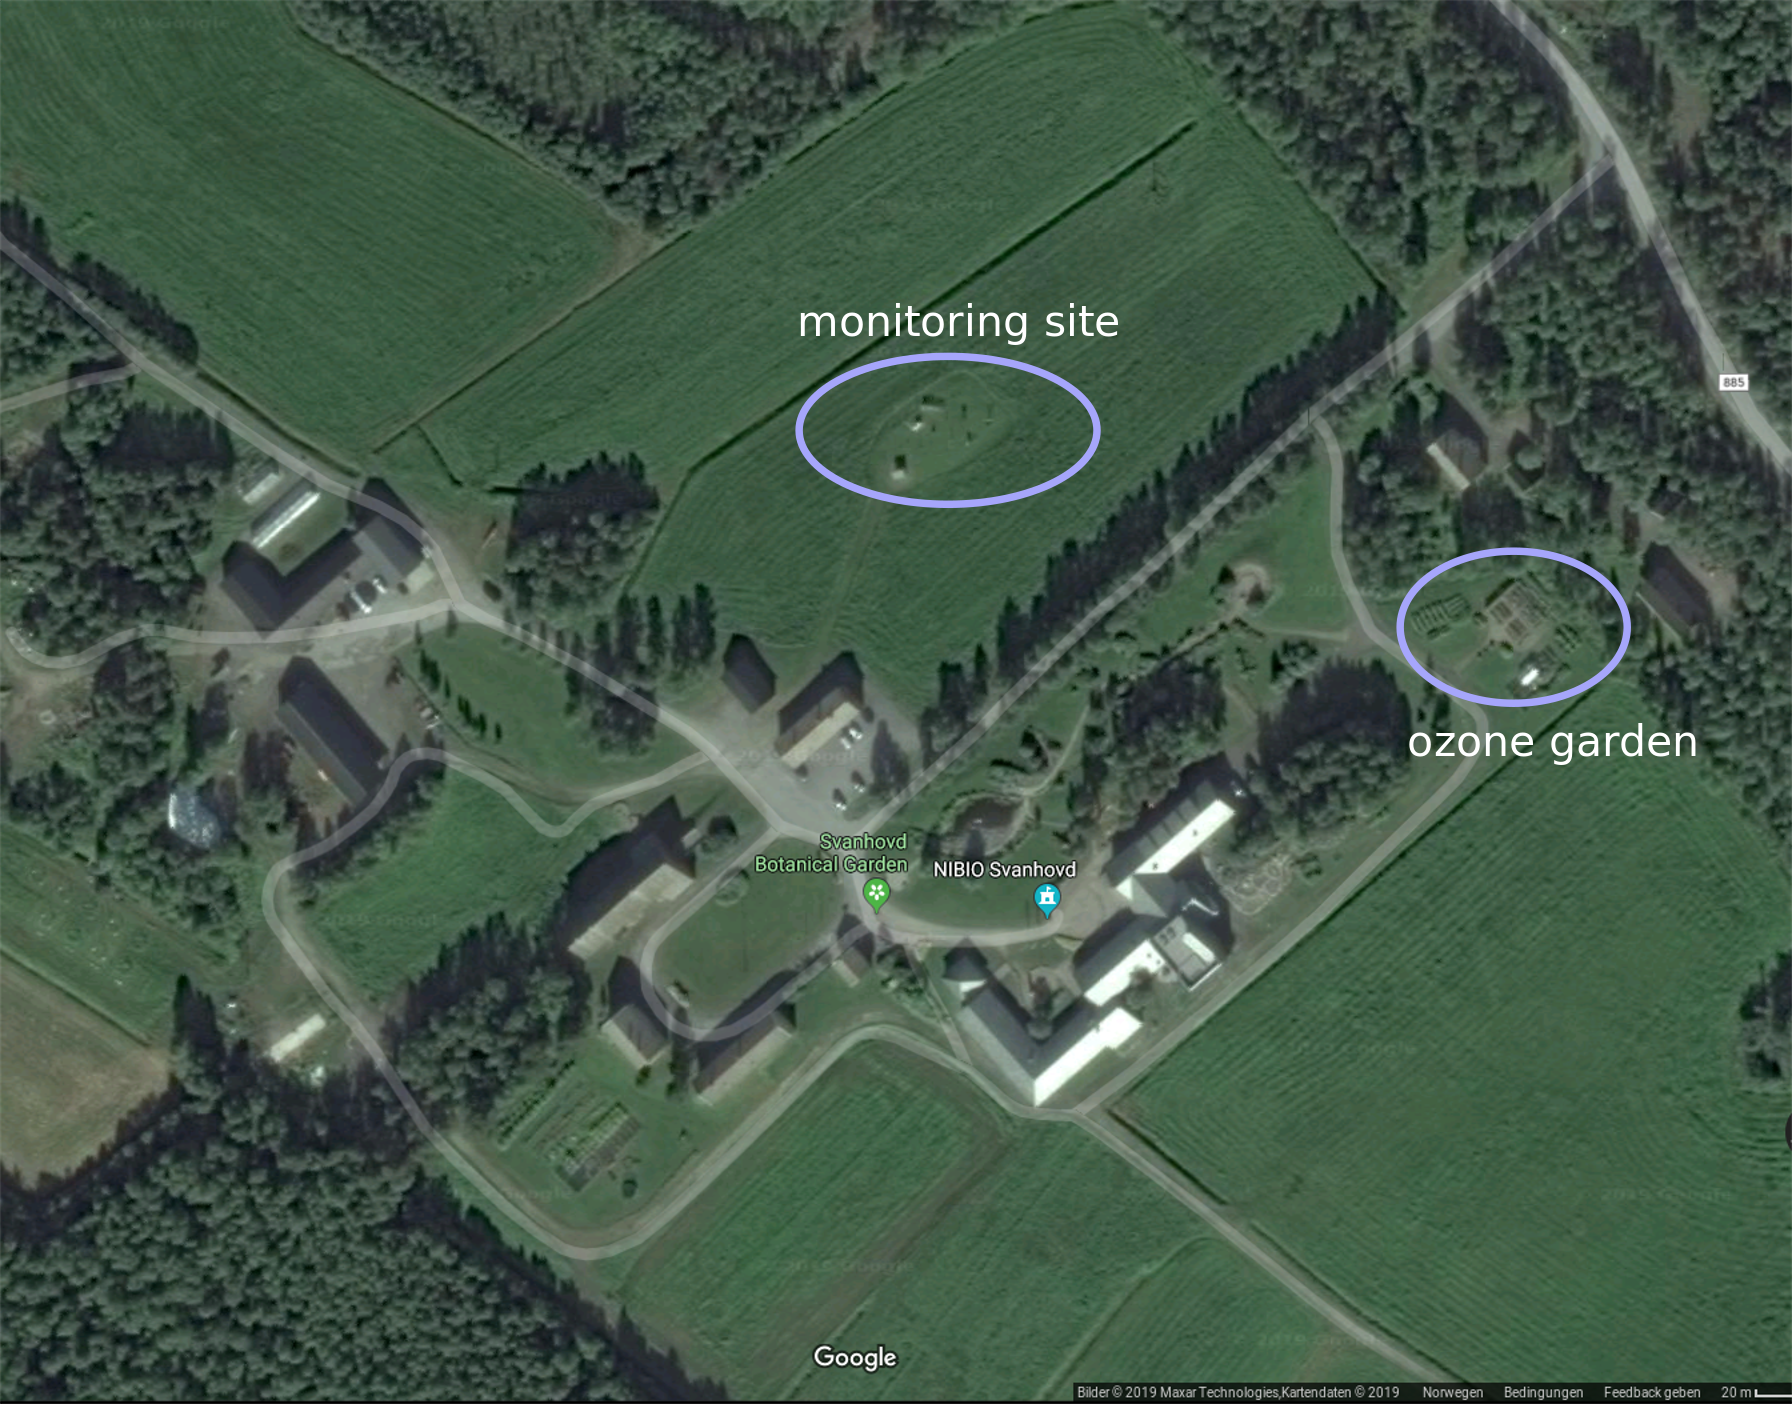
\includegraphics[width=8.3cm]{svanhovd_researchstation}\\
  (b)\\
  \includegraphics[width=8.3cm]{IMG_7739.JPG}
  %\includegraphics[width=8.3cm]{fig01}
  \caption{NIBIO Environment Centre Svanhovd close by the settlement of Svanvik, Norway. (a) Atmospheric monitoring site and ozone garden have been marked. Aerial photography \copyright Norges Kartverk; (b) Clovers in the Svanhovd ozone garden. The plants had to be secured against herbivores with a wire-mesh fence. The plants shown are approximately $6-12\,\unit{cm}$ high.}
  \label{fig:svanhovd_research_station}
\end{figure}

%%%
\subsection{Model parameter localization}
\label{sec:localization}

We determined the dominant species on-site at Svanhovd from Fig.~\ref{fig:svanhovd_research_station}a and found perennial grassland, birch (generalized as deciduous trees), and Scots pine (generalized as coniferous trees). Basic parameters for these PFTs are derived from \citet{EP:Simpson2007,GCB:Mills2011,ICP:MappingManual2017} and will be referred to as mapping manual (MM) parameterizations. The localization of parameters for coniferous trees is based on MM's Boreal Norway spruce, deciduous trees on MM's silver birch, and perennial grassland on MM's perennial grassland for Central Europe. For a comprehensive list of MM parameters, consult Supplement~Table~S1. In the following, we suggest localizations of key environmental parameters to a subarctic climate based on meteorological data to assess over-/underestimation of ozone damage when using MM Boreal parameterizations in ozone risk assessments.

\subsubsection{Temperature and light response}

Initial simulations with the MM parameterizations for perennial grassland revealed an unexpected low stomatal conductance at leaf-level ($G_\mathrm{sto}^\mathrm{leaf}$) in 2019 (Appendix~Fig.~\ref{fig:pody_mm_composit}). Substantial stomatal conductance occurred only during an extended warm period in late July. In ecological terms, this means that there would have been almost no growth of grass in the summer of 2019 -- a model prediction that is falsified by reality. We identified $f_\mathrm{T}$ as abnormally low throughout the season, being the limiting factor of stomatal conductance in perennial grassland. This suggested that a localization of the parameterization to a subarctic climate was necessary.

To localize the temperature response function $f_\mathrm{T}$, we divided the temperature dataset into two subsets: 1992--2000 (near past) and 2011--2019 (present). From these two subsets, we selected only dates within the GS (May--September) and plotted the probability density functions (PDFs) as histograms with $1\,\unit{^\circ C}$ binning (Fig.~\ref{fig:f_temp_grassland}a). A comparison between the two PDFs indicates that the temperature distribution has shifted towards higher temperatures reducing the number of days below $5\,\unit{^\circ C}$. It is unclear how fast the species composition of perennial grassland responds to these changes. Thus, the predominant acclimation at present is not known. Further, we overlaid these histograms with the MM $f_\mathrm{T}$. A low overlapping area suggests a low agreement with local climate conditions. 

Hence, the idea was to define localized temperature response functions by increasing the overlapping area between $f_\mathrm{T}$ and the temperature PDF during the GS. To this end, we defined two different hypothetical target species: subarctic and cold. We constructed \emph{cold} as representative for a species that is more tolerant to cold temperatures than MM, but slightly less efficient at warm temperatures than MM. This was accomplished by moving $T_\mathrm{min}$ and $T_\mathrm{opt}$ towards cooler temperatures but $T_\mathrm{max}$ was kept at its MM value. In the same way, \emph{subarctic} was constructed to represent a species that is very tolerant to cold but sensitive to high temperatures, and most efficient at cool temperatures. Therefore, we shifted both $T_\mathrm{min}$ and $T_\mathrm{max}$ to colder temperatures and chose $T_\mathrm{opt}$ close to the climatological mean temperature of 1992--2000. The most extreme of the two localizations compared to MM is \emph{subarctic}.

For localizing $f_\mathrm{light}$, we presumed that the opening extent of stomata at low light conditions differs in subarctic species compared to species in less extreme climates. We, therefore, adjusted the modelled light sensitivity of stomata such that the PPFD value needed to reach $50\,\unit{\%}$ opening is varied by $\pm 20\,\unit{\%}$. For this, we derive the inverse function $f_{\mathrm{light},k}^{-1}$ of Eq.~(\ref{eq:flight}) for each PFT $k$ analytically
%
\begin{equation}
  \gamma_k(f_\mathrm{light}) := f_{\mathrm{light}, k}^{-1} = -\frac{\ln(1-f_\mathrm{light})}{\alpha_k}.
  \label{eq:inverse_function}
\end{equation}
%
First, we solved Eq.~(\ref{eq:inverse_function}) for the MM default value of $\alpha_\mathrm{MM}^k$ at $0.5$ ($50\,\%$ opening)
\begin{equation}
  \gamma^k(0.5) = -\frac{\ln(0.5)}{\alpha_\mathrm{MM}^k},
  \label{eq:inverse_function_halfway}
\end{equation}
and defined a variation $\gamma' = \gamma \cdot \eta$ with $\eta \in \{0.8, 1.2\}$. By solving Eq.~(\ref{eq:inverse_function}) for $\alpha$, we find $\alpha'(\gamma')$. 

In Fig.~\ref{fig:f_temp_grassland}b, we show the PPFD PDF for near past and present together with the $f_\mathrm{light}$ for perennial grassland. The MM parameterization is displayed as solid line. 

\begin{figure}[t]
  \centering
  (a)\\
  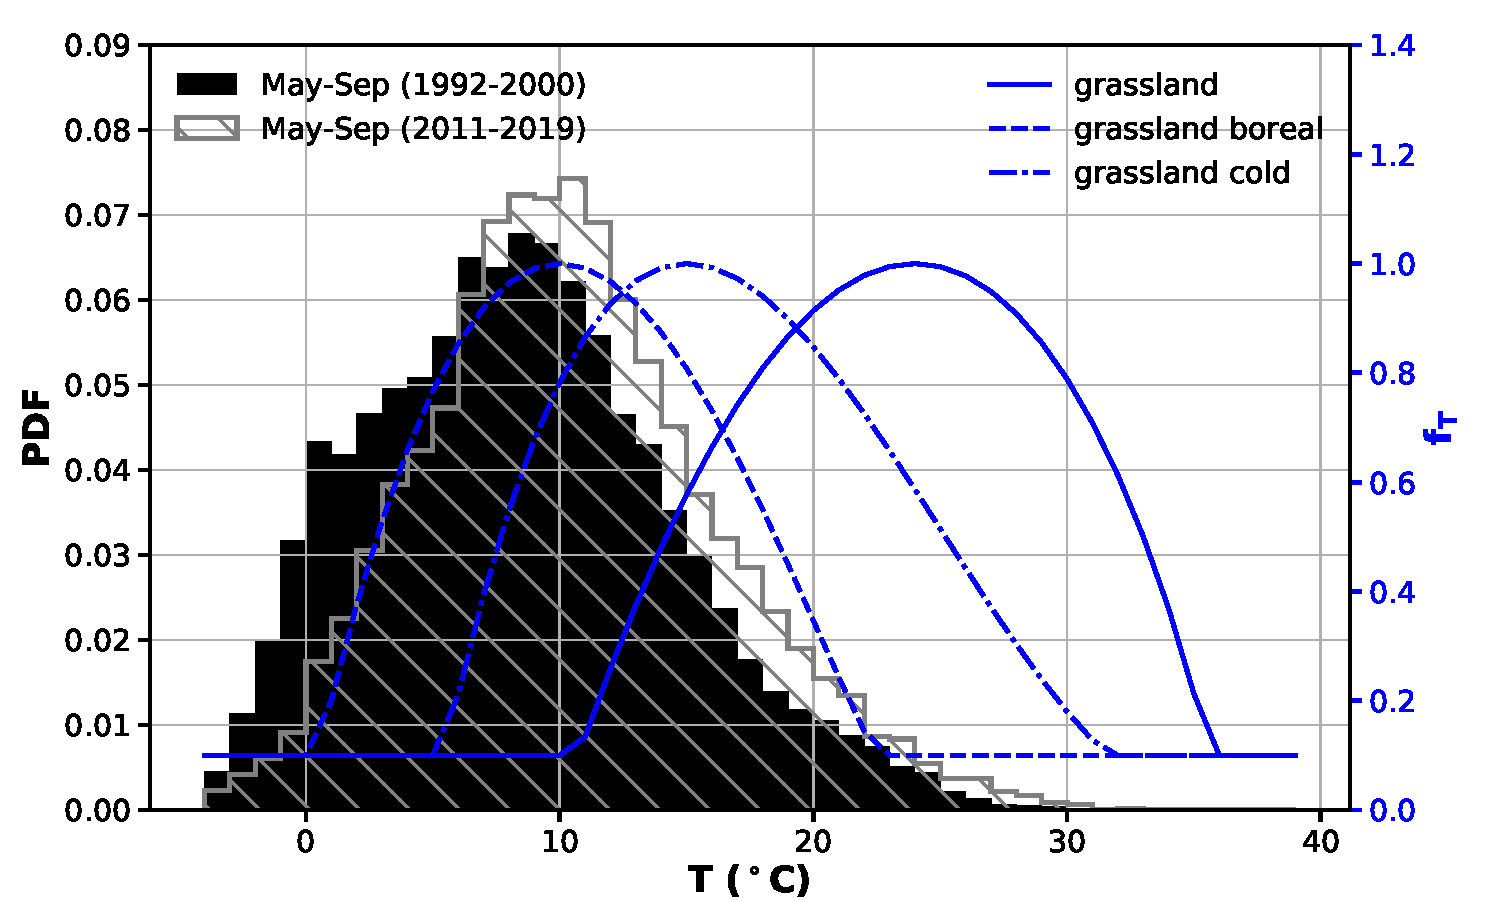
\includegraphics[width=8.3cm]{javis_funcs_temp_hist_grassland}\\
  (b)\\
  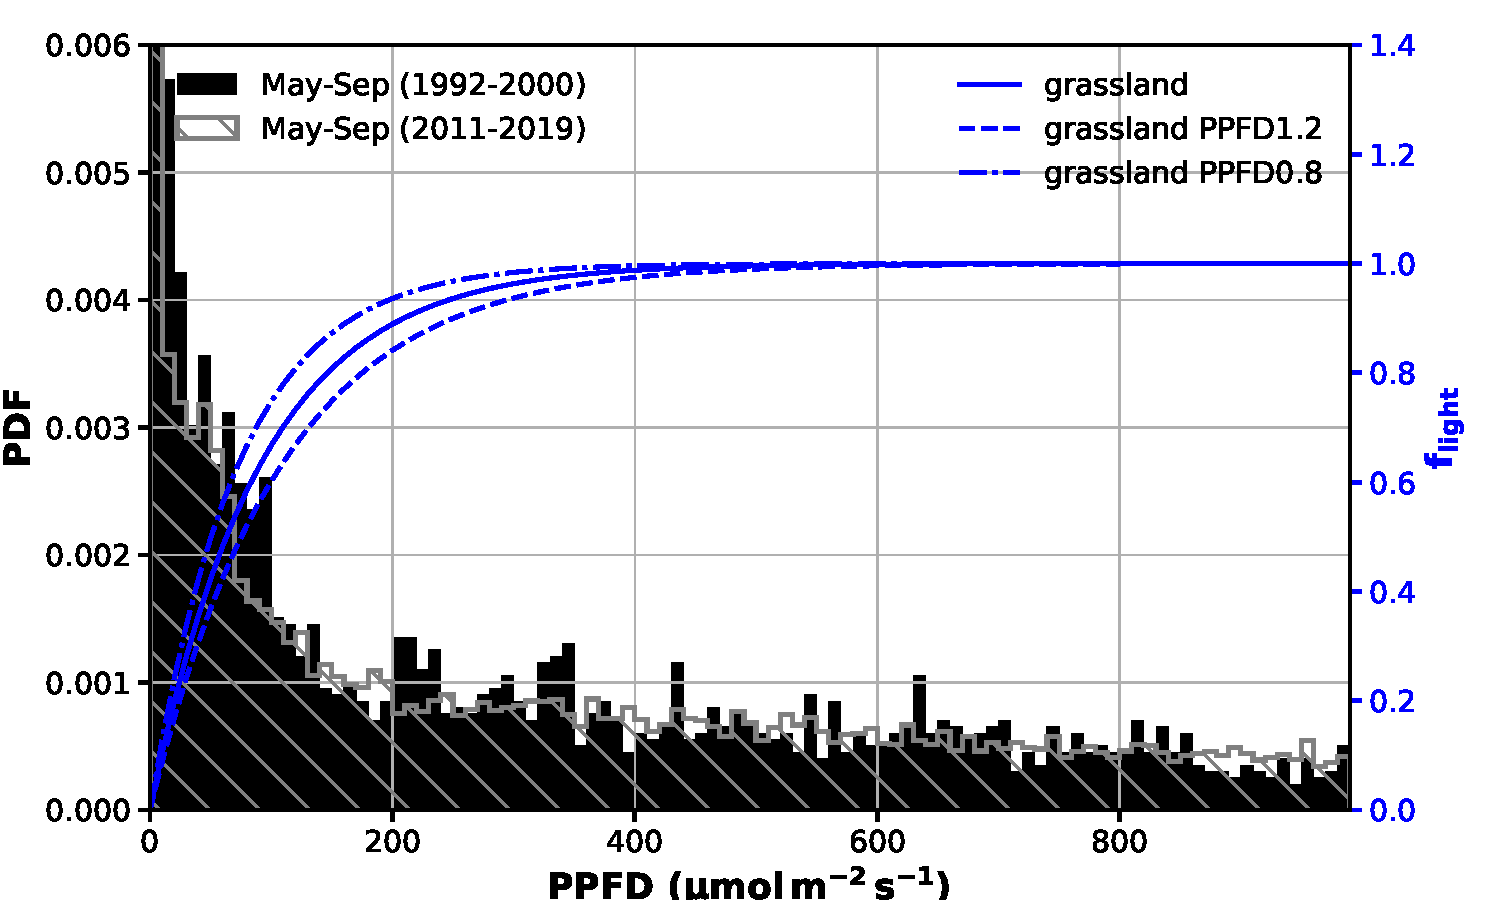
\includegraphics[width=8.3cm]{javis_funcs_light_hist_grassland}
  %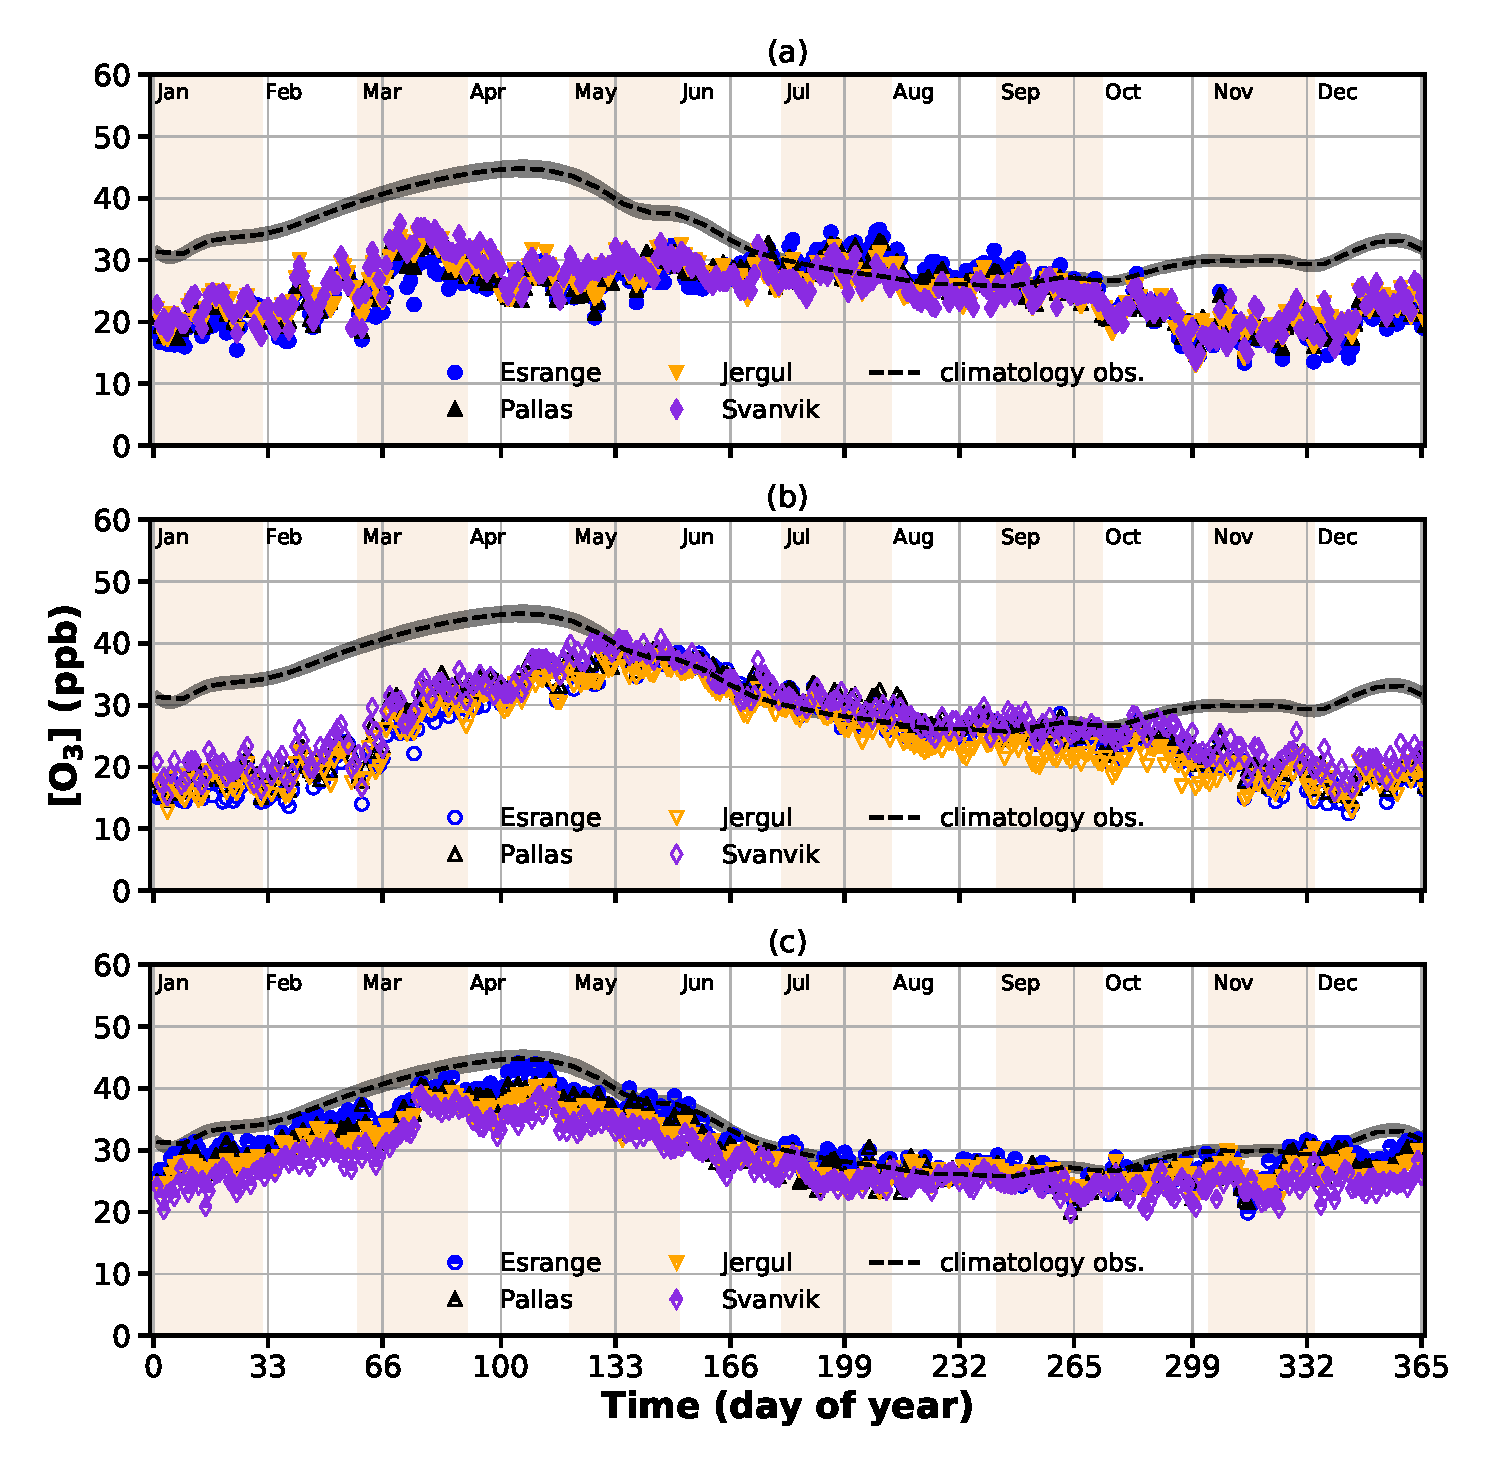
\includegraphics[width=8.3cm]{fig07}
\caption{Construction of bespoke response functions for grassland. (a) $f_\mathrm{T}$ and (b) $f_\mathrm{flight}$ are shown together with underlying $T_\mathrm{air}$ and $Q_0$ climatologies (probability density function - PDF), respectively. Original mapping manual parameterization is shown in comparison as solid line. Note that $Q_0$ has been truncated to $0.006$. PPFD0.8 and PPFD1.2 refer to $\alpha$ values increasing/decreasing PPFD at $f_\mathrm{light}=0.5$ by $\pm 20\,\%$, respectively.}
\label{fig:f_temp_grassland}
\end{figure}

Similarly, we defined localized $f_\mathrm{T}$ and $f_\mathrm{light}$ for coniferous and deciduous trees. The resulting response functions are shown in Appendix~Figs.~\ref{fig:f_temp_spruce} and \ref{fig:f_temp_birch}, respectively.
Coniferous trees are known to start photosynthesis as soon as the leaf temperature reaches a certain threshold \citep{TB:Kolari2007}. Thus, coniferous trees are already active at low air temperatures and can reach $60\,\unit{\%}$ photosynthetic activity as early as \unit{doy}~100 but cease activity in less favorable conditions \citep{TB:Kolari2007, TP:Wallin2013}. 
To determine the temperature localization for coniferous trees, we used the time series of \chem{CO_2} uptake and temperature at observation sites in southern ($\rightarrow$ \emph{cold}) and northern ($\rightarrow$ \emph{subarctic}) Finland by \citet{TB:Kolari2007}. From these, we estimated an optimal temperature interval ($10\,\unit{^\circ C}\le T_\mathrm{opt} \le 15\,\unit{^\circ C}$). For simplicity, the same interval was assumed for deciduous trees.

All resulting temperature response function localizations are tabulated in Table~\ref{tab:sensitivity_tests_temp} and light response function in Table~\ref{tab:sensitivity_tests_light}. In Section~\ref{subsec:res_local}, we compare relative $g_\mathrm{sto}$ based on Eq.~(\ref{eq:stomatal}) for the different localizations using the long term meteorological data.

\begin{table}[t]
  \caption{Bespoke temperature parameterizations. MM refers to mapping manual \citep{GCB:Mills2011,ICP:MappingManual2017}.}
  \label{tab:sensitivity_tests_temp}
  \begin{tabular}{llrrr}
    \tophline
    Species & type & $T_\mathrm{min}$ & $T_\mathrm{opt}$ & $T_\mathrm{max}$ \\
    \middlehline
    \multirow{3}{*}{Deciduous tree} & MM & 5 & 20 & 100\\
    & Cold & 5 & 15 & 100\\
    & Subarctic & 0 & 10 & 100\\
    \middlehline
    \multirow{3}{*}{Coniferous tree} & MM & 0 & 20 & 100\\
    & Cold & 0 & 15 & 100\\
    & Subarctic & 0 & 10 & 100\\
    \middlehline
    \multirow{3}{*}{Perennial grassland} & MM & 10 & 24 & 36\\
    & Cold & 5 & 15 & 36\\
    & Subarctic & 0 & 10 & 24\\
    \bottomhline
    \end{tabular}
\end{table}

\begin{table}[t]
  \caption{Bespoke light parameterizations. MM refers to mapping manual \citep{GCB:Mills2011,ICP:MappingManual2017}.}
  \label{tab:sensitivity_tests_light}
  \begin{tabular}{llcr}
    \tophline
    Species & type & $\alpha$ & $\gamma(0.5)$\\
    \middlehline
    \multirow{3}{*}{Deciduous tree} & MM & 0.004 & 165.035\\
    & PPFD0.8 & 0.005 & 132.028\\
    & PPFD1.2 & 0.003 & 198.042\\
    \middlehline
    \multirow{3}{*}{Coniferous tree} & MM & 0.006 & 115.525\\
    & PPFD0.8 & 0.008 & 92.420\\
    & PPFD1.2 & 0.005 & 138.629\\
    \middlehline
    \multirow{3}{*}{Perennial grassland} & MM & 0.011 & 63.013\\
    & PPFD0.8 & 0.014 & 50.411\\
    & PPFD1.2 & 0.009 & 75.616\\
    \bottomhline
    \end{tabular}
\end{table}

\subsubsection{Growing season estimate}
\label{subsec:gs_est}

The accumulation of ozone dose is strongly depended on the timing and length of the GS. \citet{ICP:MappingManual2017} suggest a simple latitude model for beech, birch, and Norway spruce for the localization of GS:
%
\begin{align}
  A_\mathrm{start} &= 105 + (LAT-50\,\unit{^\circ N})\cdot 1.5\\
  A_\mathrm{end} &= 297 - (LAT-50\,\unit{^\circ N})\cdot 2
\end{align}
%
At Svanhovd, this yields $A_\mathrm{start}=135\,\unit{doy}$ and $A_\mathrm{end}=257\,\unit{doy}$. We verified these as follows.

For coniferous trees, we used a MODIS (Aqua/Terra) retrieved GPP product \citep{MODIS_PSN} on a $1\times 1\,\unit{km}$ patch centered at Svanhovd. GPP over time follows approximately a second-order polynomial function (Fig.~\ref{fig:modis_gpp}). By calculating the roots of the fitted polynomial, we found $A_\text{start}$ as \unit{doy}~122 for 2018 and \unit{doy}~106 in 2019. $A_\text{end}$ amounts to \unit{doy}~261 and 274, respectively. This $A_\mathrm{end}$ value will be used for all PFTs alike. The resulting growing season for coniferous trees in 2019 was one month longer than in 2018. For $A_\text{start}$ of deciduous trees, we use temperature-degree-days (above $5\,\unit{^\circ C}$) on gridded temperature data from SeNorge.no (Appendix~Fig.~\ref{fig:greening_season_change_Svanvik}). We found \unit{doy}~129 and 130, respectively. For both years, these dates coincide with the first snow-free day at the closest inland meteorological weather station at Øvre~Neiden (Sør-Varanger, NOR) and are very similar to the latitude model predictions. For perennial grassland, we assume a latency period of $1\,\unit{month}$ after snow-melt. This assumption is supported by observations in Rovaniemi, Finland \citep[][Supplement~Fig.~S1]{FCR:Korhonen2018}. All results are tabulated in Table~\ref{tab:sensitivity_tests_gs}.

\begin{table}[t]
  \caption{Start and end of growing season in \unit{doy}. Central Europe is shown for comparison.}
  \label{tab:sensitivity_tests_gs}
  \begin{tabular}{lcll}
    \tophline
    Species & Year & $A_\mathrm{start}$ & $A_\mathrm{end}$\\
    \middlehline
    Central Europe$^b$ & -- & 100 & 307\\
    Latitude model ($70\,\unit{^\circ N}$)$^b$ & -- & 135 & 257\\
    \multirow{3}{*}{Deciduous tree} & 2018 & 129$^*$ & 261$^a$ \\
    & 2019 & 130$^c$ & 274$^a$ \\
    & 2100 & 116$^e$ & 286$^e$ \\
    \multirow{2}{*}{Coniferous tree} & 2018 & 122$^a$ & 261$^a$ \\
    & 2019 & 106$^a$ & 274$^a$ \\
    \multirow{2}{*}{Perennial grassland} & 2018 & 159$^d$ & 261$^a$\\
    & 2019 & 161$^d$ & 274$^a$ \\
    \bottomhline
  \end{tabular}
  \belowtable{$^a$ MODIS (Aqua/Terra) GPP product;\\
    $^b$ \citet{ICP:MappingManual2017},\\
    $^c$ $5\,\unit{days}-5\,\unit{^\circ C}$-rule, $T_\mathrm{air}$ from \href{seNorge.no}{seNorge.no};\\
    $^d$ One month after snowmelt; reference station Øvre Neiden (Sør-Varanger, NOR)\\
    $^e$ Future projection based on linear regression of $^c$ (Fig.~\ref{appendix:growing_season})
    } % Table Footnotes
\end{table}

\subsubsection{Other properties}
\label{subsec:soil}

Soil texture influences water availability and thus $\mathrm{POD_y}$ calculations in $\mathrm{DO_3SE}$ \citep{ACP:Bueker2012}. The soil at Svanhovd is characterized in an ICP~Forest plot survey as gleyic cambisols according to the Food and Agriculture Organization of the United Nations (FAO) soil classification system and as eluviated dystric brunisol in the ICP~Forest soil classification system (V. Timmerman, personal communication, June 2020). The clay:sand:silt content is estimated to range from 12\,\%:61\,\%:27\,\% at the top layer to 16\,\%:59\,\%:25\,\% in about $1\,\unit{m}$ depth (\href{https://soilgrids.org/}{soilgrids.org}, last accessed April 2022 for location $30.0334\,\unit{^\circ E}$, $69.4549\,\unit{^\circ N}$) Within the $\mathrm{DO_3SE}$ soil parameterization, the sandy loam texture describes the upper $60\,\unit{cm}$, where the plant roots are found, of this soil type best. 

We did not perform a localization of the water vapor pressure deficite $f_\mathrm{VPD}$ and soil water potential $f_\mathrm{SWP}$ response functions. But acknowledge that these are very important factors in the modeling of ozone dose as pointed out by~\citet{ACP:Bueker2012}.

The quasi-laminar boundary layer resistance $R_b$ is a function of wind speed $u$ and influenced by the tree height and leaf dimensions. For comparison with MM, we collected a sample of birch (B. pubescence) leaves from the outer canopy (good light exposure) of tall trees at two sites in Finnmark. The leaves were collected late in July, thus, they were fully expanded. They were collected by hand at about $2\,\mathrm{m}$ height. As the sun is at a low elevation angle for most of the time in the growing season in this area, light exposure at the top of the tree is not expected to be different from lower leaves as long as they grow in a part of the tree that is not shadowed by other trees. At the first site (Karasjok), three leaves were collected from five adult trees each. At the second site (Svanvik), five leaves were collected from one tree. The leaves were pressed and dried before scanning for the area and shape determination through image analysis. ImageJ (\href{https://imagej.nih.gov/ij/}{see webpage}) was used for thresholding the images to give silhouettes of the leaves. After scaling the images, the program was used to find the minimum Feret diameter. This measure finds the largest width of a leaf at a $90^\circ$ angle to the length of the leaf (the Feret diameter). With this method we found that the 20 leaves had a mean width of $(3.0\pm 0.5)\,\unit{cm}$ that is smaller than in the MM parameterization ($5\,\unit{cm}$, Supplement~Table~S1). 

A report by \citet[][p.~52]{NINA2004} indicated an average tree height of $13.5\,\unit{m}$ in the Svanhovd area. One Scots pine forest at Svanhovd has been studied as a part of the ICP Forest mapping. There, heights were measured in 2004 when the stand was 90~years old. The mean tree height was $10.1\,\unit{m}$ and maximum height was $16.2\,\unit{m}$ (V. Timmerman, personal communication, June 2020). We used $13.5\,\unit{m}$ for both deciduous and coniferous trees as this height is found from a larger and more diverse population of species.

\section{Results}
\label{sec:results}
In this section, we first compute the average stomatal conductance $\left<g_\mathrm{sto}\right>$ relative to $g_\mathrm{max}$ for each PFT from the long term meteorological data according to Eq.~(\ref{eq:stomatal}) and compare the different localizations to MM (Section~\ref{subsec:res_local}). We use the $\mathrm{DO_3SE}$ model to compute the ozone dose and projected biomass loss due to ozone for the two recent GSs 2018/19 for each species and localization (Section~\ref{subsec:do3se_results}). Finally, we put the results into a climatological perspective (Section~\ref{subsec:climatologies}).  

\subsection{Parameter localization}
\label{subsec:res_local}

We presume that perennial vegetation will likely maximize carbon acquisition during the short subarctic growing season. Because the MM version of the $\mathrm{DO_3SE}$ model currently does not simulate net photosynthesis $A_\mathrm{n}$, we assume a first order proportionality between $A_\mathrm{n}$ and $g_\mathrm{sto}$ \citep{GCB:Medlyn2011}. A higher average $\left<g_\mathrm{sto}\right>/g_\mathrm{max}$ ratio, thus, indicates a higher growth potential in the local climate.

We propose the following metric. From the long term of meteorological data, we select two distinct periods: noon ($11\,\unit{am}-1\,\unit{pm}$ local time) and morning ($5-9\,\unit{am}$ local time) and calculate the average relative stomatal conductance $\left<g_\mathrm{sto}\right>/g_\mathrm{max}$ (Eq.~(\ref{eq:stomatal}) assuming $f_\mathrm{SWP}=1$). Presumably, $\left<g_\mathrm{sto}\right>/g_\mathrm{max}$ around noon (the highest light intensity) is a good proxy for \chem{CO_2} uptake efficiency (growth). In addition, a small deviation between noon and morning and a low standard deviation indicates higher robustness of this localization to variability in growing conditions. From left to right in Fig.~\ref{fig:javis_func_opt_mean}, results using the subarctic, cold, and MM $f_\mathrm{T}$ are shown marked by an alternating background color. Within each of these groups $f_\mathrm{light}$ categories are indicated by PPFD0.8 and PPFD1.2, respectively. The standard deviation is denoted with error bars. 

Based on the above criteria, we identify \emph{subarctic}--PPFD0.8 as the parameterization with the highest score. The differences between the localized parameterizations and the MM are smallest for coniferous trees. This indicates that the MM Boreal parameterization is well suited for the subarctic climate at Svanhovd. For perennial grassland, the differences compared to MM are largest suggesting that the MM Central European parameterization is not appropriate in a subarctic climate. Deciduous trees display also a notable increase in mean stomatal conductance using our localizations.

\begin{figure}[t]
  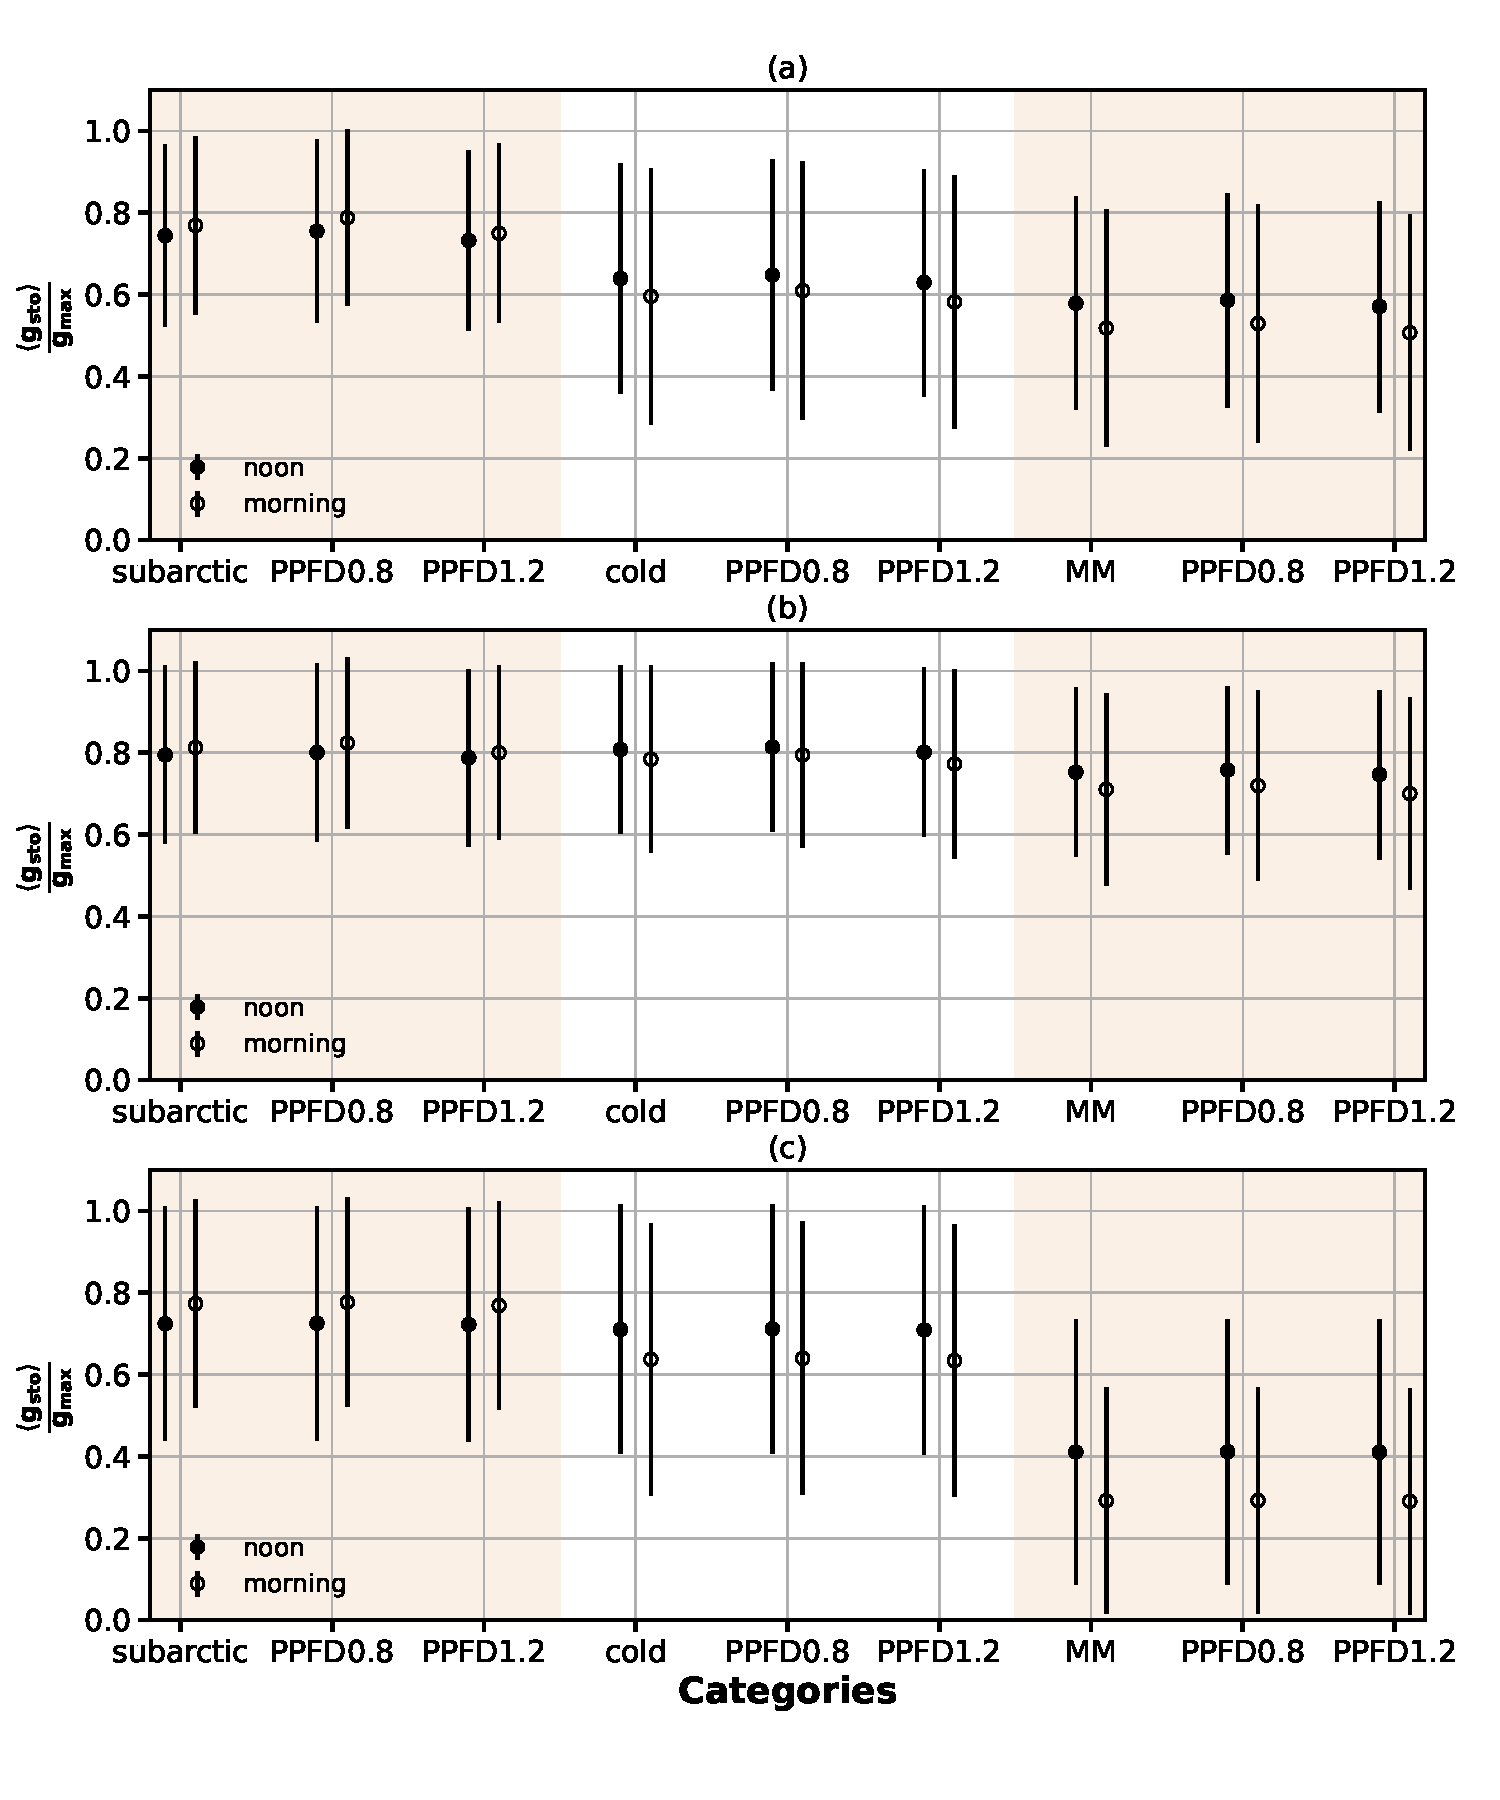
\includegraphics[width=8.3cm]{javis_func_opt_mean}
  %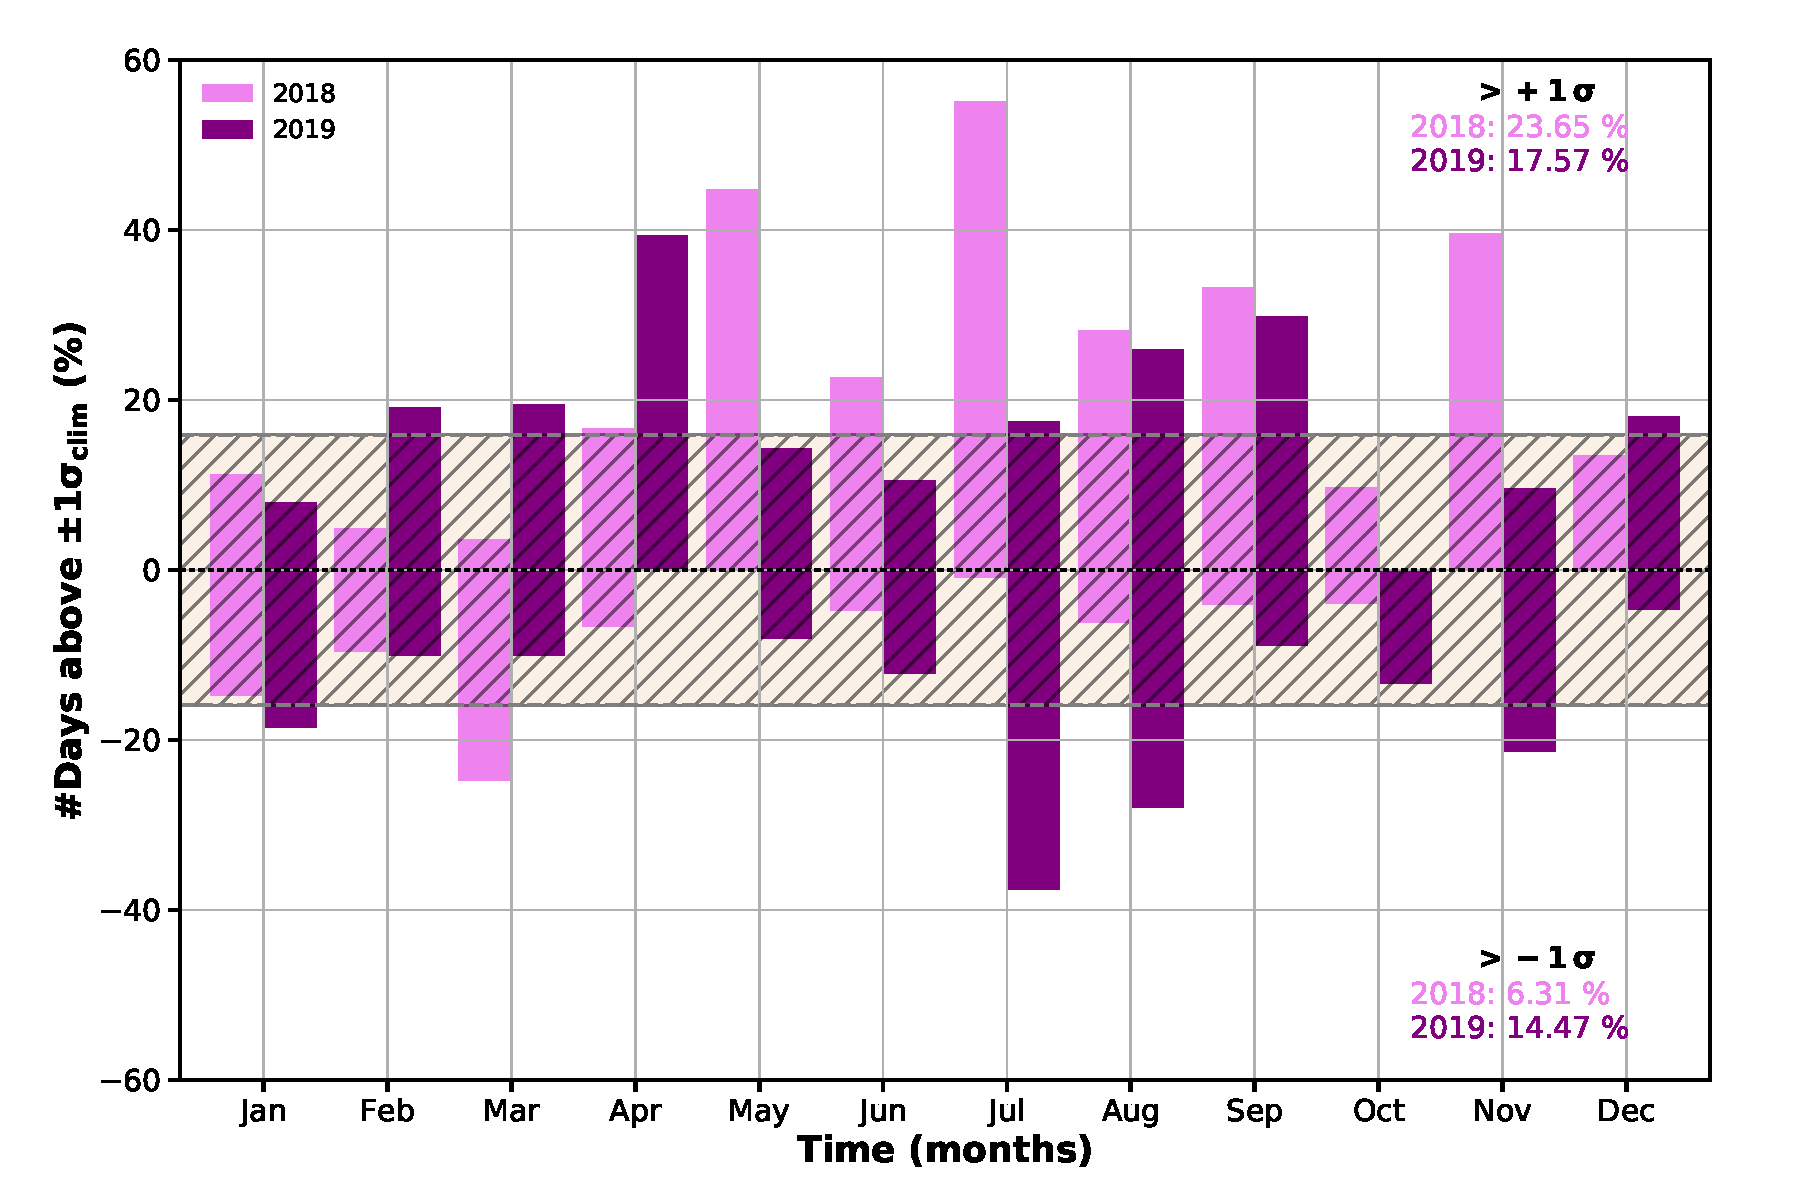
\includegraphics[width=8.3cm]{fig08}
  \caption{Proposed metric to test bespoke response functions. GS (May--August) climatological averages and standard deviation of $g_\mathrm{sto}^k$ (Eq.~(\ref{eq:stomatal})) relative to $g_\mathrm{max}^k$ at noon (averaged over $11\,\unit{am}-1\,\unit{pm}$ local time) and in the morning (averaged over $5-9\,\unit{am}$ local time) are shown for (a) deciduous trees; (b) coniferous trees; (c) perennial grassland.}
  \label{fig:javis_func_opt_mean}
\end{figure}

\subsection{Implications on ozone risk assessments}
\label{subsec:do3se_results}

We modeled $\mathrm{POD_y}$ with a flux threshold $y=1\,\unit{nmol\,m^{-2}\,s^{-1}}$ per PLA for the three natural/semi-natural vegetation types, deciduous trees, coniferous trees, and perennial grassland using the MM parameterization and our localized temperature (\emph{cold}, \emph{subarctic}) and light (PPFD0.8, PPFD1.2) parameterizations. 

The results are comprehensively displayed in Fig.~\ref{fig:pody_rel}. Critical levels for reduction in biomass \citep[deciduous forest $4\,\unit{\%}$, coniferous forest $2\,\unit{\%}$, and grasslands $10\,\unit{\%}$ biomass reduction adopted from][]{ICP:MappingManual2017,ESPR:Hayes2021} are shown as horizontal dashed lines. The different background colors indicate the temperature response function localization. The light response function localizations are denoted by $+$ (PPFD1.2) and $-$ (PPFD0.8). Circles indicate simulations with localized GS, canopy height, and leaf dimensions, TODO: (whereas squares indicate simulations with MM GS for Central Europe. We chose this to demonstrate the impact of a projected prolonged GS in the future.) With open symbols, the effect on $\mathrm{POD_y}$ with SWP taken into account is displayed.

We identified in general that an increasing cold tolerance represented by a shift in the temperature response function (MM $<$ cold $<$ subarctic) leads to an increase in $\mathrm{POD_1}$ in both probed years. TODO: (while using locally adapted GS causes a reduction.) An earlier start and overall longer GS in 2019 leads to higher $\mathrm{POD_1}$ compared to 2018 despite the occurrence of more episodes of elevated \chem{O_3} in 2018 than in 2019 (see Section~\ref{subsec:anomalies} for details). Taking into account SWP, $\mathrm{POD_1}$ was effectively only reduced for deciduous trees in 2018, while in all other cases simulation results with and without SWP effects were identical. An earlier opening of stomata at low light intensities (PPFD0.8) caused an increase in $\mathrm{POD_1}$ compared to MM while a later opening (PPFD1.2) reduced $\mathrm{POD_1}$. Due to the shape of $f_\mathrm{light}$, a symmetric variation can lead to an asymmetric response in $\mathrm{POD_1}$.

For deciduous trees (Fig.~\ref{fig:pody_rel}a) all $\mathrm{POD_1}$ simulations exceed the CL by TODO: ($5-25\,\unit{mmol\,\chem{O_3}\,m^{-2}}$) and display the largest spread in $\mathrm{POD_1}$ with respect to $f_\mathrm{light}$. In 2019, the lowest estimated $\mathrm{POD_1}$ (MM, PPFD1.2) amounts to $10\,\unit{mmol\,\chem{O_3}\,m^{-2}}$, while the highest estimate (subarctic, PPFD0.8) reaches about $20\,\unit{mmol\,\chem{O_3}\,m^{-2}}$. In 2018, this uncertainty range is much smaller ($(12-18)\,\unit{mmol\,\chem{O_3}\,m^{-2}}$). In particular, the impact of $f_\mathrm{light}$ is pronounced (extent of $\angle(+,0,-)$). The maximum difference in $\mathrm{POD_1}$ due to the $f_\mathrm{light}$ localization for the PPFD0.8 (superscript) and PPFD1.2 (subscript) amount to $^{+1.6}_{-2.3}\,\unit{mmol\,\chem{O_3}\,m^{-2}}$ for 2018 and $^{+1.9}_{-2.7}\,\unit{mmol\,\chem{O_3}\,m^{-2}}$ for 2019. The difference in $\mathrm{POD_1}$ compared to MM in response to the localization of $f_\mathrm{T}$ and GS ranges between $\Delta\mathrm{POD_1}=(1.4-3.6)\,\unit{mmol\,\chem{O_3}\,m^{-2}}$ in 2018 and $\Delta\mathrm{POD_1}=(2.7-7.7)\,\unit{mmol\,\chem{O_3}\,m^{-2}}$ in 2019. A low soil water potential caused a reduction in $\mathrm{POD_1}$ in 2018 in cases when using PPFD0.8. This indicates that drought conditions can reduce the ozone damage risk. TODO: (With MM GS, $\mathrm{POD_1}$ values were higher in 2018 than in 2019. However, taking the localized GS into account, this is reversed for the subarctic temperature response function. This can be explained by more favorable growing conditions in 2019.) 

For coniferous trees (Fig.~\ref{fig:pody_rel}b), most simulations slightly exceed the CL ($0-10\,\unit{mmol\,\chem{O_3}\,m^{-2}}$). Our localization does not show much difference compared to MM indicating the the MM Boreal Norway spruce parameterization was already well-adjusted to the local subarctic climate. We find a higher $\mathrm{POD_1}$ in 2019 than in 2018. The maximum difference in $\mathrm{POD_1}$ determined between localized GS for subarctic and cold parameterizations with respect to MM ranges between $(0.5-1.0)\,\unit{mmol\,\chem{O_3}\,m^{-2}}$ in 2018 and $(2.0-3.3)\,\unit{mmol\,\chem{O_3}\,m^{-2}}$ in 2019. The maximum difference determined from PPFD0.8 (superscript) and PPFD1.2 (subscript) $f_\mathrm{light}$ amounts to $^{+1.0}_{-0.8}\,\unit{mmol\,\chem{O_3}\,m^{-2}}$ for 2018 and $^{+1.3}_{-1.0}\,\unit{mmol\,\chem{O_3}\,m^{-2}}$ for 2019.

For perennial grassland (Fig.~\ref{fig:pody_rel}c), all simulations with localize GS stay below the CL. Perennial grassland shows the smallest $\mathrm{POD_1}$, but a similarly large response to the temperature parameterization localizations as deciduous trees. Again, we find a reversal for predicted ozone risk in 2018 and 2019 for the subarctic type. Perennial grassland shows the lowest sensitivity to the light threshold. TODO: (and SWP is only relevant without localized GS (see above).) The overall difference in $\mathrm{POD_1}$ determined from the localized GS for subarctic and cold types with respect to MM ranges between $(2.2-3.4)\,\unit{mmol\,\chem{O_3}\,m^{-2}}$ in 2018 and $(4.4-6.4)\,\unit{mmol\,\chem{O_3}\,m^{-2}}$ in 2019. The chosen lower maximum temperature in the subarctic parameterization probably caused the lower $\mathrm{POD_1}$ in 2018 (warm year) compared to the cold parameterization. This was not seen in 2019. The maximum difference in $\mathrm{POD_1}$ determined from the PPFD0.8 (superscript) and PPFD1.2 (subscript) variation of $f_\mathrm{light}$ amount to $^{+0.3}_{-0.2}\,\unit{mmol\,\chem{O_3}\,m^{-2}}$ and $^{+0.3}_{-0.3}\,\unit{mmol\,\chem{O_3}\,m^{-2}}$, respectively.

The maximum difference in $\mathrm{POD_1}$ between simulations with the MM parameterizations and the localized temperature and light response functions is of the same order of magnitude as the difference between the two probed years. The magnitude of all described effects on $\mathrm{POD_1}$ varies between PFTs as well as years, but is by construction always larger than estimated with the MM parameterization. This means that the ozone damage risk could be possibly underestimated even in normal years and establishing dedicated subarctic parameterizations are a must to properly assess ozone damage risk in these regions.

\begin{figure}[t]
  \centering
  (a)\\
  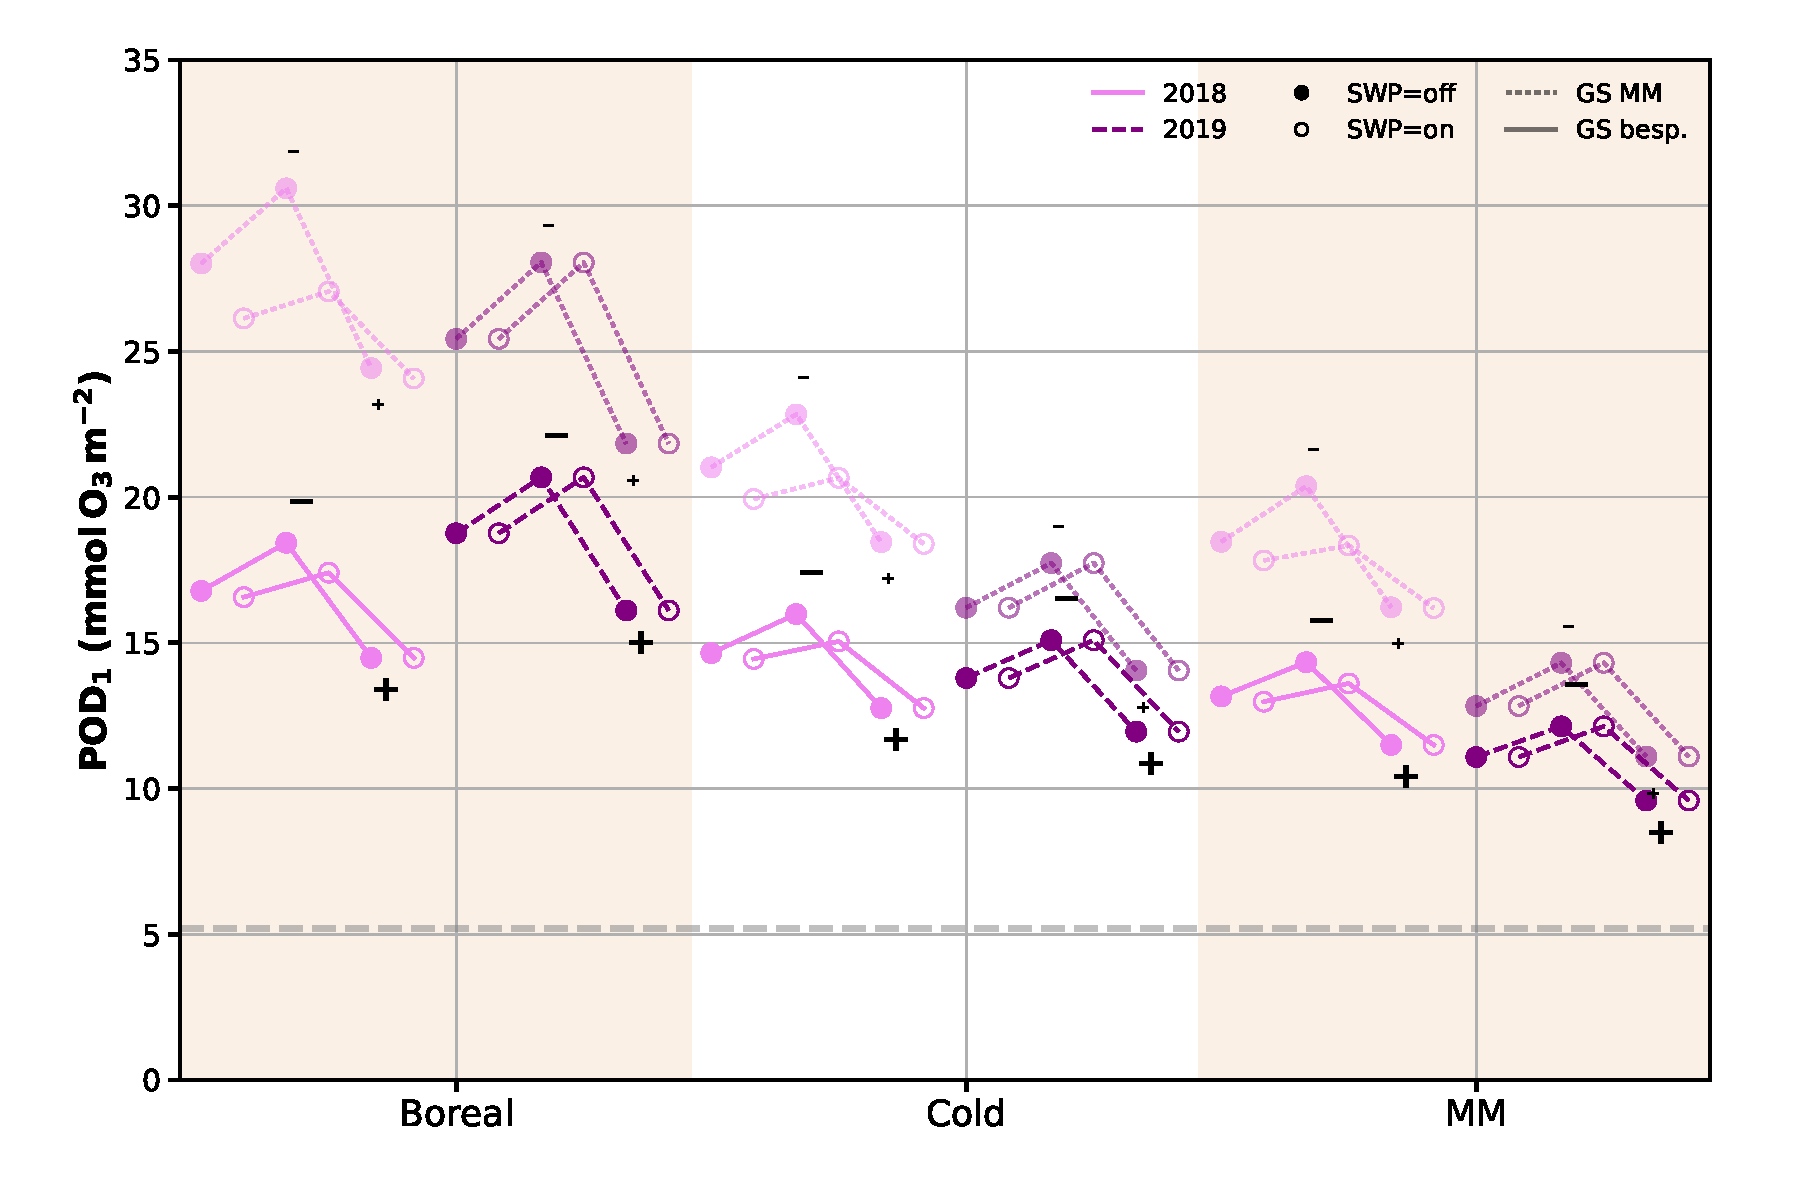
\includegraphics[width=8.3cm]{do3se_results_pod_v3_Birch.pdf}\\
  (b)\\
  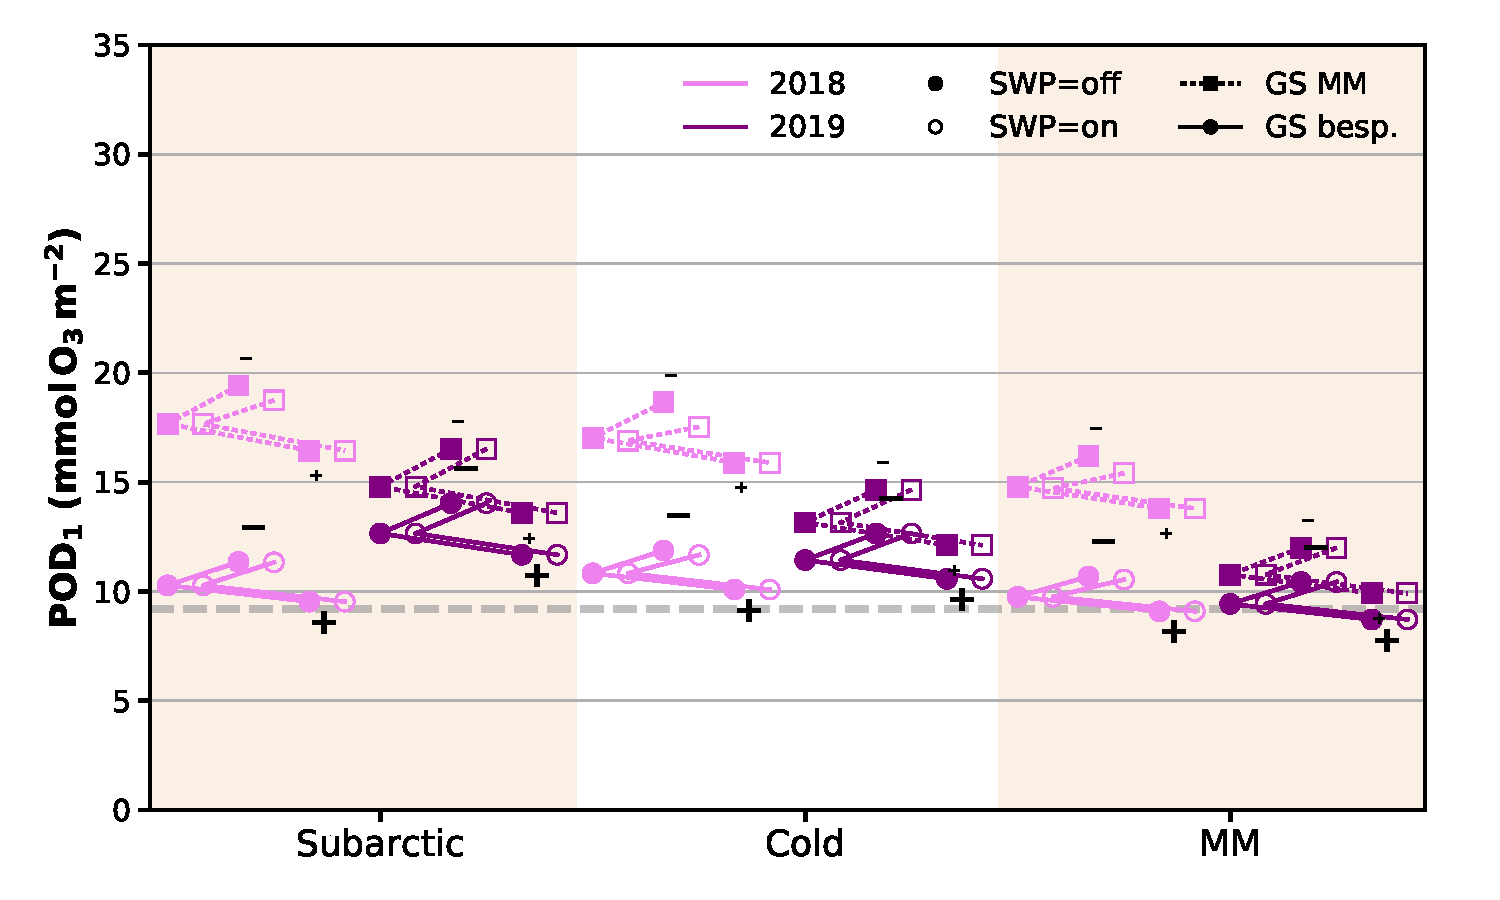
\includegraphics[width=8.3cm]{do3se_results_pod_v3_Spruce.pdf}\\
  (c)\\
  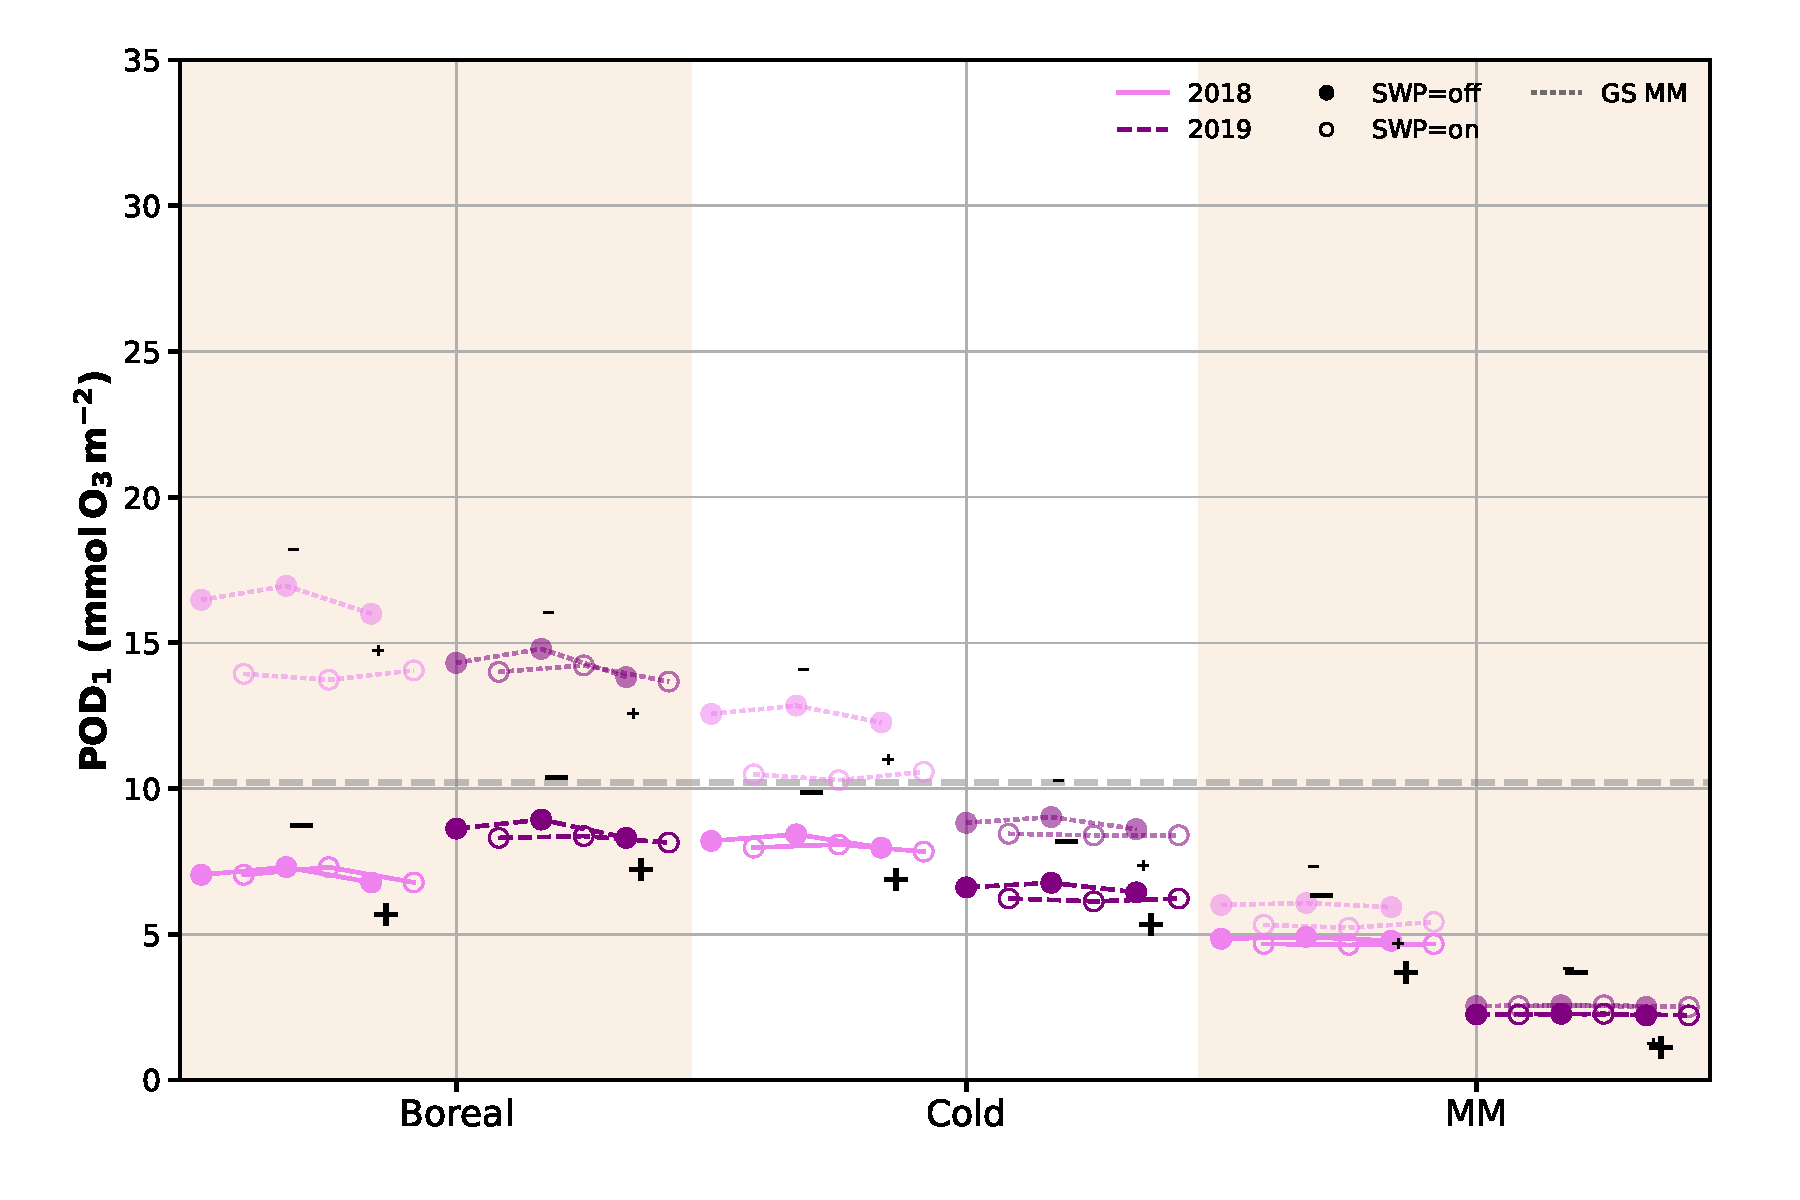
\includegraphics[width=8.3cm]{do3se_results_pod_v3_Grassland.pdf}
  %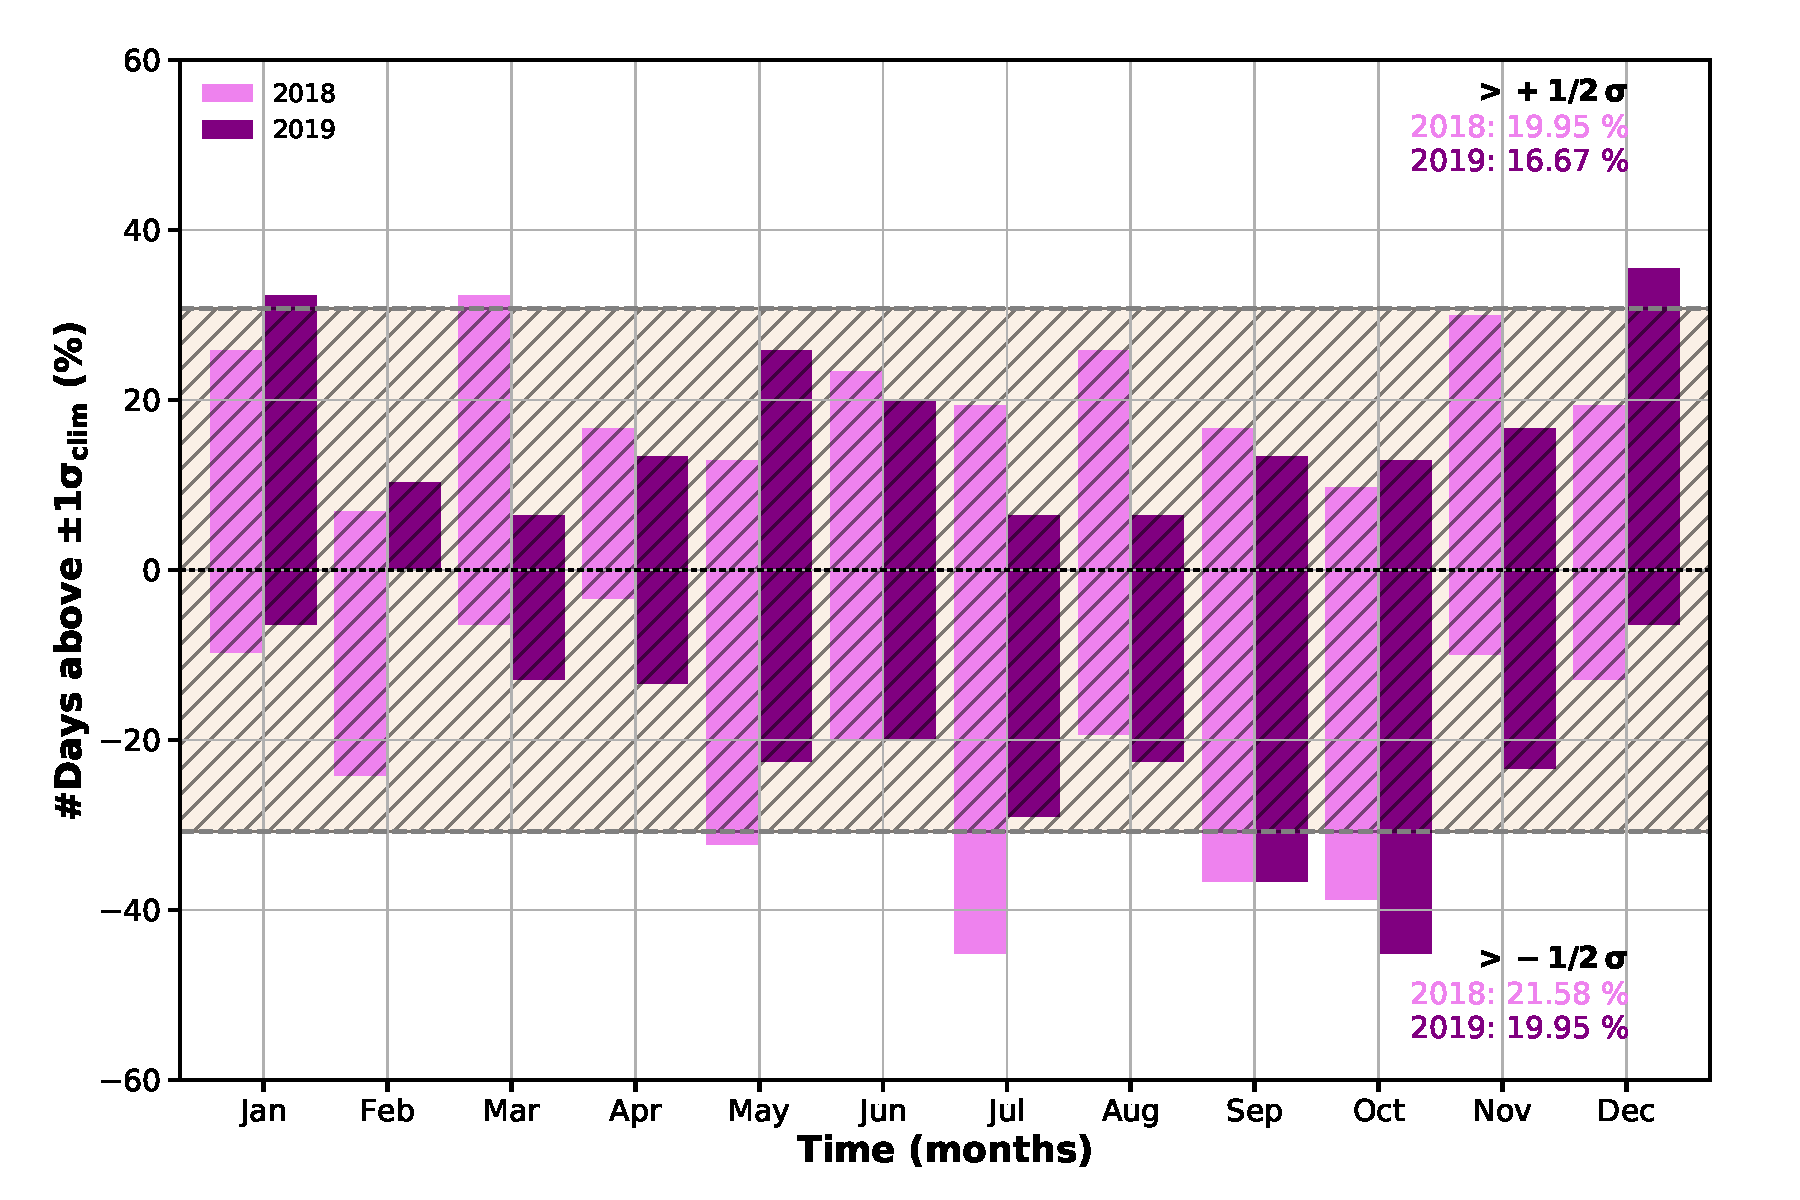
\includegraphics[width=8.3cm]{fig09}
  \caption{$\mathrm{DO_3SE}$ modeling $\mathrm{POD_1}$ results for (a) deciduous trees, (b) coniferous trees, and (c) perennial grasslands at Svanhovd in 2018 (pink) and 2019 (purple). The results varied depending on parameterizations of temperature response functions (MM, Cold, and Subarctic, details in Table~\ref{tab:sensitivity_tests_temp}), growing season (GS MM (squares) or GS bespoke (circles), details in Table~\ref{tab:sensitivity_tests_gs}), light response functions (first, second and third point attached by a line are depicting the MM, PPFD0.8 and PPFD1.2, details in Table~\ref{tab:sensitivity_tests_light}), and the effect of taking SWP into account (filled symbols without and open symbols with effects of drought kept in the model). Critical levels for ozone damage \citep{ICP:MappingManual2017,ESPR:Hayes2021} are given as dashed horizontal lines. Note that the horizontal axis is only categorical.}
  \label{fig:pody_rel}
\end{figure}

We estimated the biomass reductions in accordance to the CLs \citep{ICP:MappingManual2017, ESPR:Hayes2021} for the most extreme temperature parameterization localization (\emph{subarctic}) for each PFT. The estimates for SWP=off are listed in Table~\ref{tab:biomass_reduction}. We defined an uncertainty range from the difference in biomass reduction caused by the variation of $f_\mathrm{light}$. Superscript refers to PPFD0.8 and subscript to PPFD1.2. The reported range corresponds to the effect of taking SWP into account or not. As SWP reduces $\mathrm{POD_1}$, biomass reduction is decreased when taking SWP into account. The biomass reduction ranges between $2.5\,\unit{\%}$ (coniferous, 2018) and $17.4\,\unit{\%}$ (deciduous, 2019). For deciduous trees this amounts to a reduction by up to $55\,\unit{\%}$ compared to MM. From an agro-economical point of view in our focus area, where the grass is cut only once a year, a loss of biomass of more than $10\,\unit{\%}$ can have severer consequences compared to more productive areas in central Europe. Therefore, CL may also need localization.
Coniferous trees are the least affected PFT and the magnitude of total biomass reduction is almost independent of the choice of the parameterization within given uncertainties.

\begin{table}[t]
  \caption{Estimated total biomass reduction in \unit{\%} for temperature acclimation \emph{subarctic} with localized GS and SWP=off. The uncertainty ranges reported here correspond to maximum a divergence deducted from varying $f_\mathrm{light}$ and SWP=on. For comparison, the corresponding biomass reduction for the MM parameterization averaged over both years is shown. In this case, standard deviation is computed from all sensitivity simulations ($\pm 20\,\unit{\%}$ in extent of stomatal opening at low light, SWP on/off, and localized GS).}
  \label{tab:biomass_reduction}
\begin{tabular}{lllll}
\tophline
Year & \multicolumn{4}{c}{PFT}\\
& Deciduous tree& Coniferous tree & \multicolumn{2}{c}{Perennial grassland}\\
& & & total & above ground\\
\middlehline
2018 & $15.5^{+(1.9...2.1)}_{-(0.8...1.5)}$ & $2.5^{+0.2}_{-0.2}$ & $9.7^{+0.2}_{-0.2}$ & $12.4^{+0.2}_{-0.2}$\\
2019 & $17.4^{+2.5}_{-1.8}$ & $3.0^{+0.2}_{-0.3}$ & $10.5^{+(0.1...0.2)}_{-(0.0...0.1)}$ & $13.7^{+(0.1...0.3)}_{-(0.1...0.3)}$\\
\middlehline
$\left<\mathrm{MM}\right>$ & $11.2\pm 1.1$ & $2.31\pm 0.04$ & $7.5\pm 0.9$ & $9.6\pm 1.4$\\
\bottomhline
\end{tabular}
%\belowtable{$^*$ above ground biomass} % Table Footnotes
\end{table}

\subsection{Climate and weather conditions in the growing season 2018/19}
\label{sec:stats}
Here, we put the weather conditions during the growing season 2018/19 into a climatological context. All relevant data for the growing season 2018/19 are shown as time series in Fig.~\ref{fig:data_svanvik_2018_2019}. Ozone concentrations measured at $2\,\unit{m}$ height above ground are averaged hourly. The hatched areas mark times when no ozone data were recorded. Note, while the downtime during winter was planned, missing data in two weeks of July 2018 (July 9--23) were due to problems in data acquisition.

\subsubsection{Weather conditions}
\label{subsec:weather}

As can be seen in Fig.~\ref{fig:data_svanvik_2018_2019}a, \chem{\chi_{O_3}} peaks in spring (April/May) and reaches its minimum in late summer (July/August). The spring peak has not been captured completely in 2019, since data acquisition only started in late April. In summer 2018 (June--August), high ozone concentrations ($\chem{\chi_{O_3}} > 40\,\unit{ppb}$) were recorded 50 times. The highest summer ozone VMR ($\chem{\chi_{O_3}} = 50.2\,\unit{ppb}$) was measured on July~25. This coincides with the period of the most extensive forest fires in central Sweden which occurred from July~12--29 \citep{SOU2019}. However, due to the above-mentioned data acquisition problems, we missed most of the corresponding ozone data for this event and most likely also the peak \chem{\chi_{O_3}}. A method for gap-filling these data has been presented in \citet{ACP:Falk2021} and explained in Section~\ref{subsec:gap_filling}. In contrast, \chem{\chi_{O_3}} only rose 18 times above the threshold of $40\,\unit{ppb}$ during the summer of 2019. 

Hourly averaged $2\,\unit{m}$ temperatures above $20\,\unit{^\circ C}$ occurred more regularly in July 2018 than in 2019 (Fig.~\ref{fig:data_svanvik_2018_2019}b). In 2018, spring temperature regularly rose above freezing only in May, while in 2019 this occurred already early in March/April indicating a later start of the GS in 2018.
More rain events with accumulated daily precipitation ($\sum_d \mathrm{Precip}$) above $10\,\unit{mm}$ occurred in the summer of 2018 compared to 2019 (Fig.~\ref{fig:data_svanvik_2018_2019}c).
Qualitatively, global irradiance ($Q_0$) displayed in Fig.~\ref{fig:data_svanvik_2018_2019}d was higher in May and July 2018 compared to 2019, while June 2019 showed higher irradiance than in 2018. A high global irradiance, in most cases, is the result of a low cloud fraction. In both years, the maximum recorded $Q_0$ was $750\,\unit{W\,m^{-2}}$ and reached in June.

\begin{figure*}[t]
  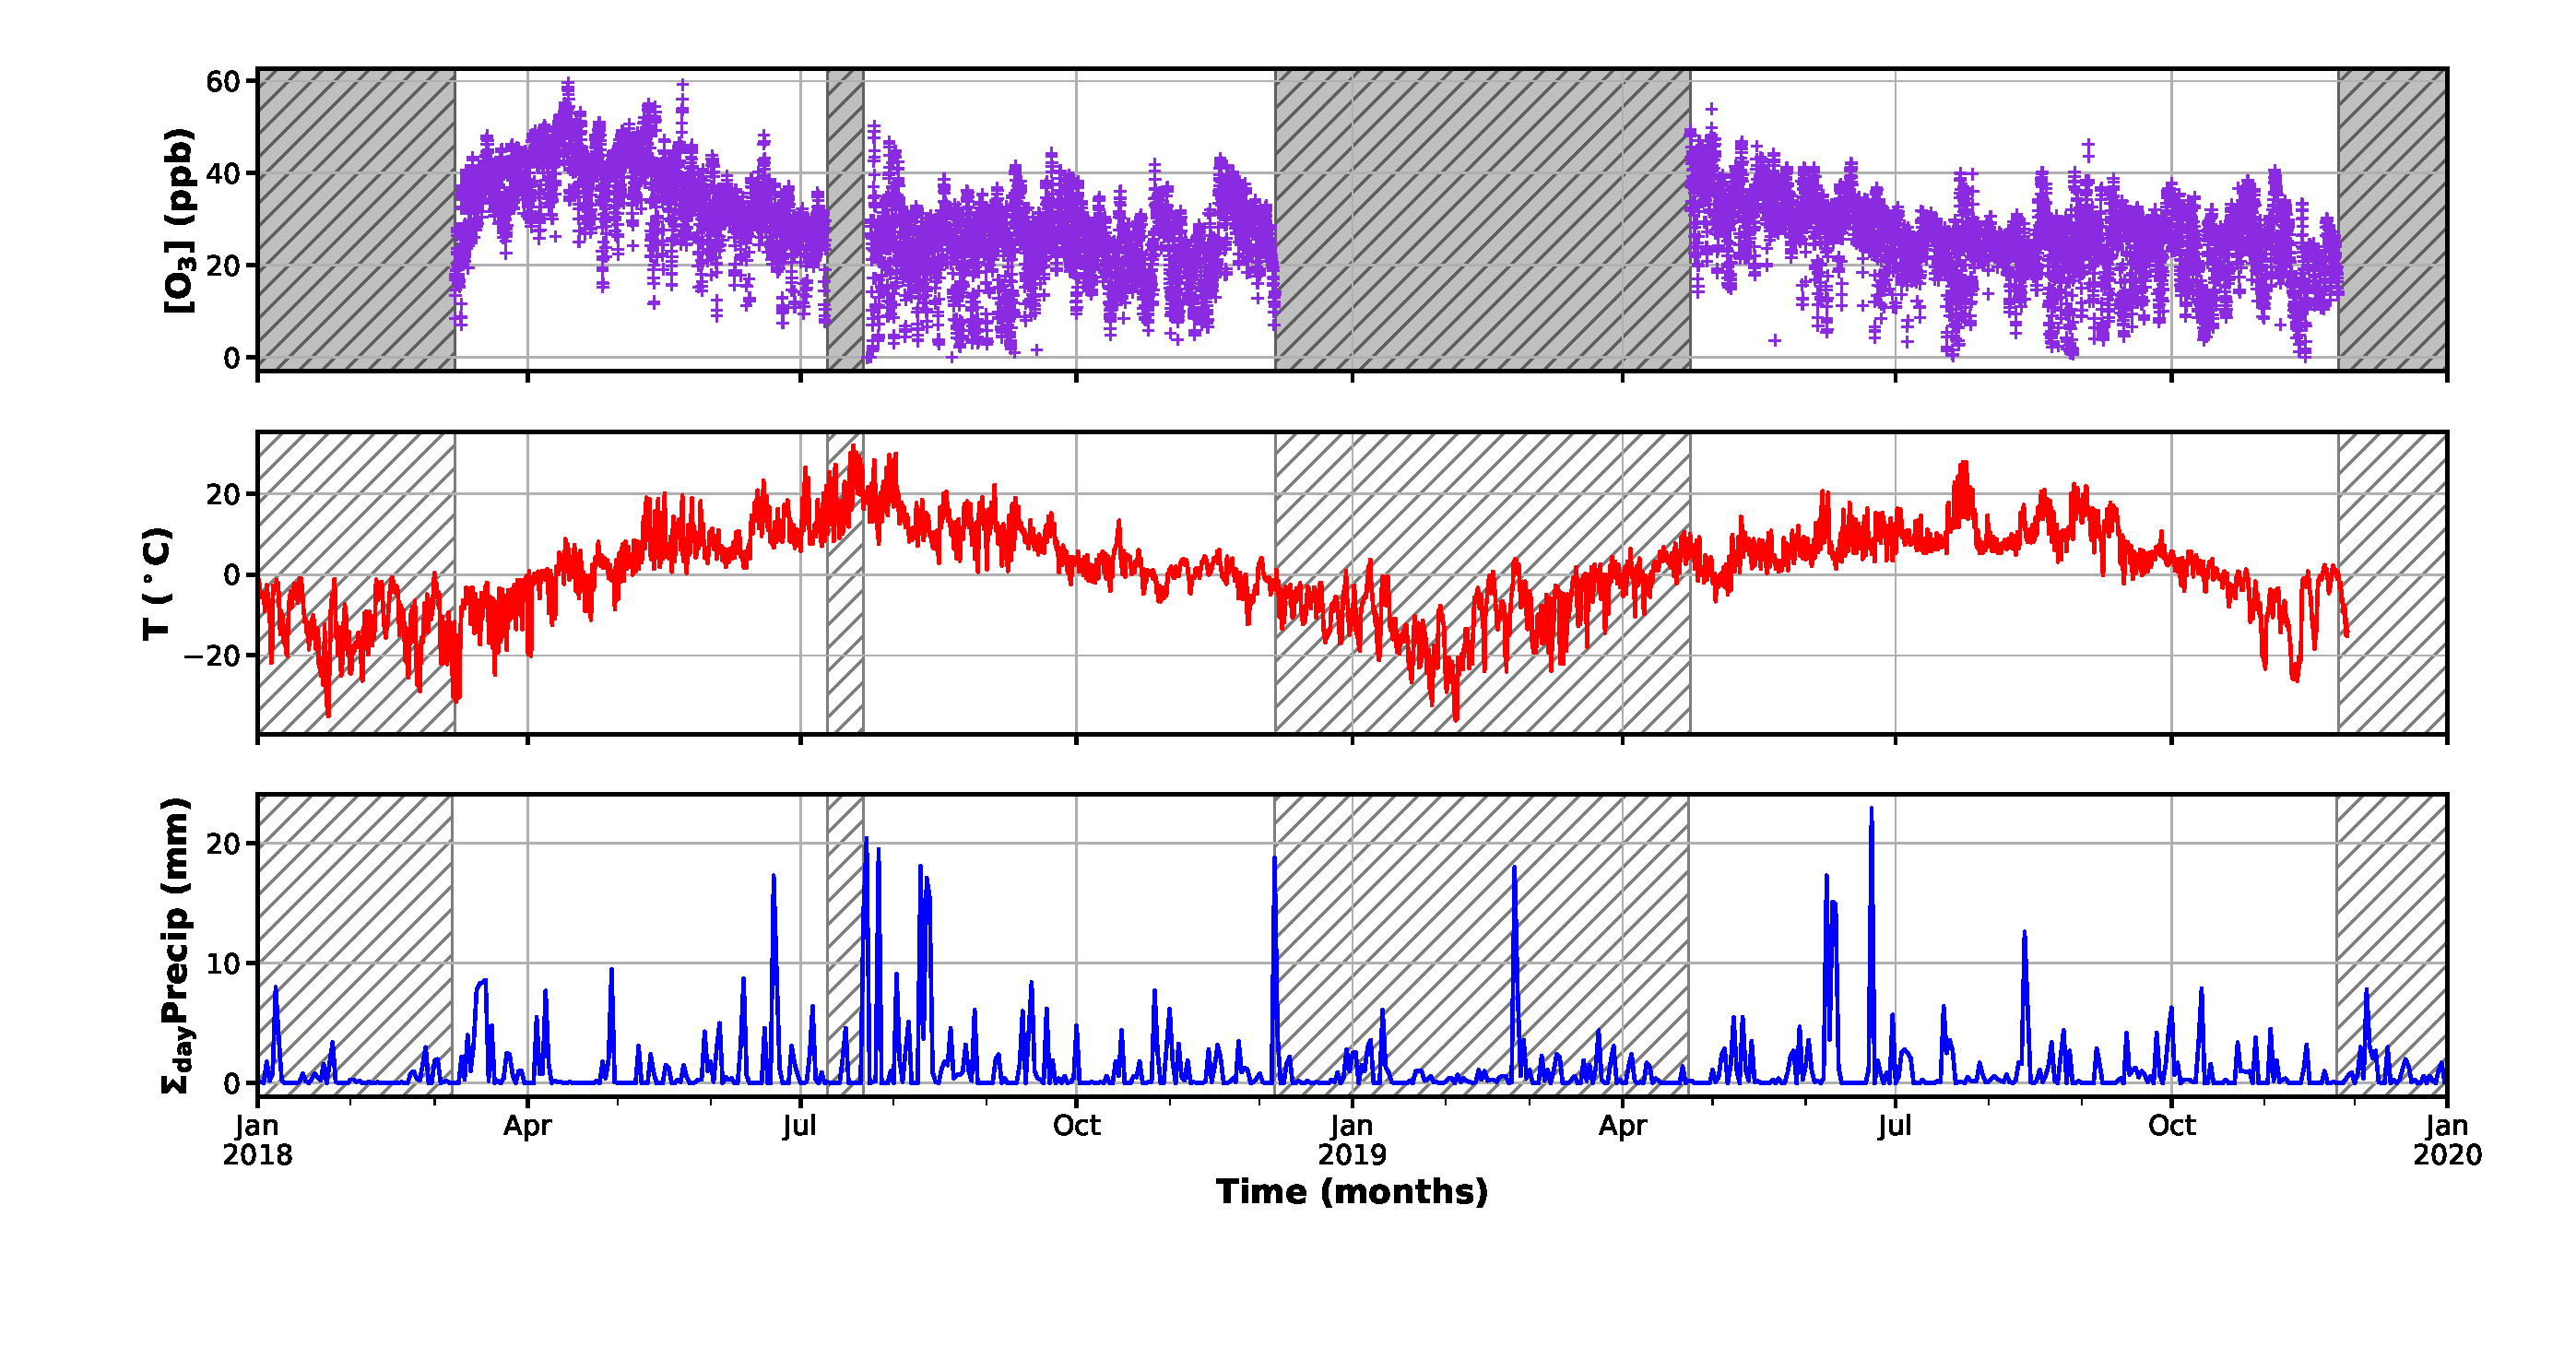
\includegraphics[width=12cm]{data_svanvik_2018_2019}
  %\includegraphics[width=12cm]{fig02}.
  \caption{Observational data from atmospheric monitoring at Svanhovd in 2018/19. The hatched areas indicate periods without ozone monitoring data. (a) Hourly averaged ozone VMR; (b) hourly averaged temperature; (c) daily accumulated precipitation; (d) hourly averaged global irradiance.}
  \label{fig:data_svanvik_2018_2019}
\end{figure*}


\subsubsection{Climate (1990-present)}
\label{subsec:climatologies}

Climatologies (typically multi-year monthly averages) of temperature, precipitation, and radiant energy $Q_\mathrm{e}$ for Svanhovd were derived for the period 1992--2012 and are shown as box plots in Fig.~\ref{fig:climatediagram}. Therein, the colored horizontal lines indicate the median and the triangles the mean value for the respective month. A box denotes the interquartile range (IQR). Observations exceeding 1.5~times the IQR (whiskers) are usually considered outliers but ought to be interpreted differently in a climate diagram, namely as events deviating extraordinarily from the norm.

Temperatures usually stay below freezing for 5 consecutive months, while only 2 months breach $10\,\unit{^\circ C}$ regularly (July, August), satisfying the conditions for a K\"{o}ppen's climate classification of a regular subarctic climate (Dfc) \citep[e.g.][]{SD:Beck2018}. The highest monthly average temperature is $(13.1\pm 1.1)\,\unit{^\circ C}$ in July and the lowest $(-12.8\pm 2.0)\,\unit{^\circ C}$ in February. The coldest ever recorded temperature was $-45.2\,\unit{^\circ C}$ on January~27, 1999, while the highest temperature ($29.4\,\unit{^\circ C}$) occurred on July~16 the same year. As can be seen mean and median are well aligned in the center of the IQR for most months meaning that temperature anomalies are symmetrically distributed.

The average accumulated monthly precipitation ($\sum_d\mathrm{Precip}$) indicates that winter and spring (November--April, except for March) are relatively dry ($\sum_d\mathrm{Precip} < 20\,\unit{mm}$). March precipitation is primarily snow and will influence the start of the growing season. The driest month is January with $\sum_d\mathrm{Precip} = (16.7\pm 3.0)\,\unit{mm}$. The most precipitation occurs in summer, with a $\sum_d\mathrm{Precip} = (58.5\pm 9.2)\,\unit{mm}$ in August. The average annual accumulated precipitation ($\sum_m\mathrm{Precip}$) given with standard error of mean is $(383\pm 86)\,\unit{mm}$. Mean and median precipitation are less well aligned compared to temperature and point to a considerable interannual variability.

The climatology for global radiant energy $Q_e$ in \unit{J\,m^{-2}} (the integral of $Q_0$) is zero in November--January (polar night) and reaches its maximum in May--July (midnight sun conditions). Mean and median are well aligned. Only June displays a slightly skewed distribution towards higher $Q_e$.

%Ozone
The ozone VMR climatology (\chem{\chi_{O_3}}) (1986--1996) is shown in Figure~\ref{fig:climatediagram}d. The climatological spring peak occurs in April (around \unit{doy} 100) and amounts to $40\,\unit{ppb}$ while the annual average \chem{\chi_{O_3}} was $28\,\unit{ppb}$. The decline in \chem{\chi_{O_3}} roughly coincides with the beginning of \chem{CO_2} uptake by coniferous trees \citep{TB:Kolari2007, TP:Wallin2013}. Mean and median are well aligned and centered indicating a symmetric distribution for each month. The highest recorded \chem{\chi_{O_3}} occur in June most likely due to forest fires as mentioned above.

\begin{figure*}[t]
  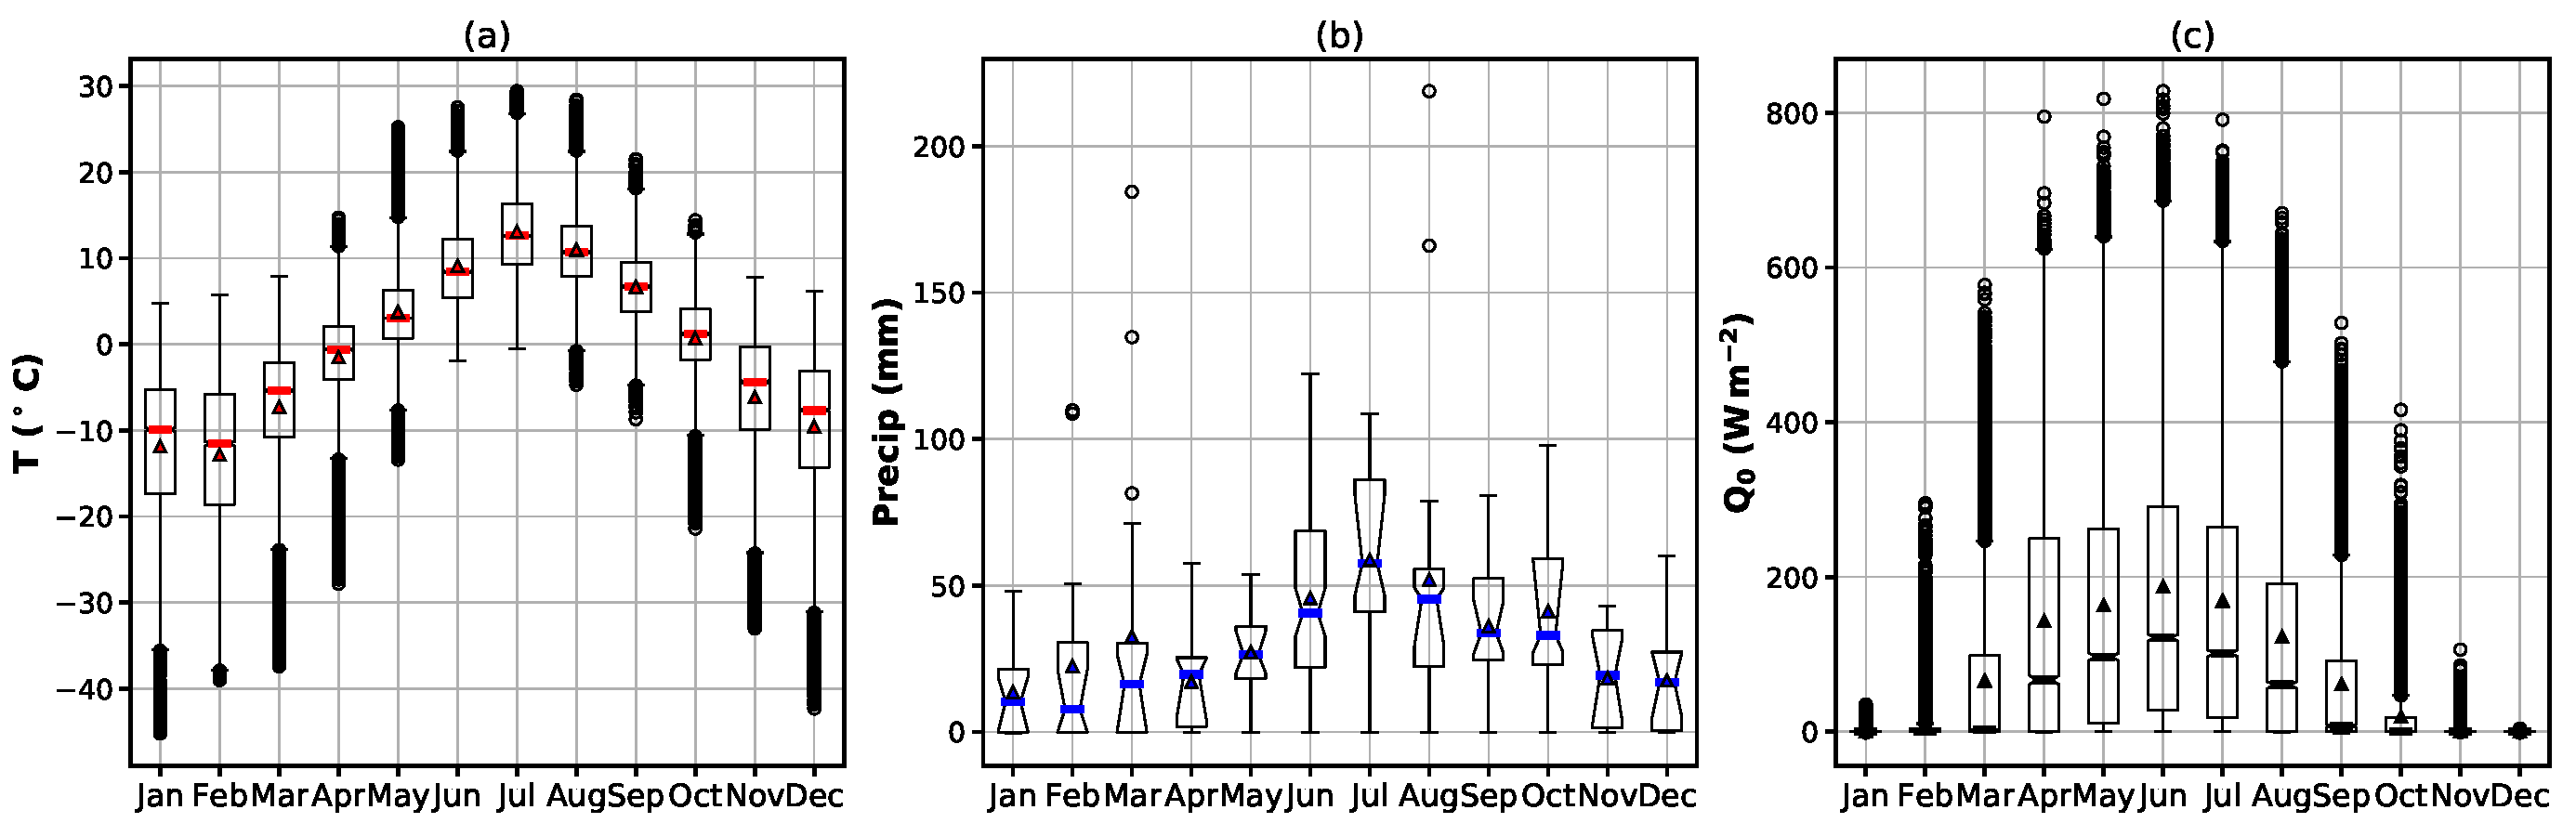
\includegraphics[width=12cm]{climatediagram_box}
  %\includegraphics[width=8.3cm]{fig04}
  \caption{Climate diagram based on meteorological data for Svanvik/Pasvik (1992--2012). Ozone climatology based on ozone monitoring data (1986--1996). A box indicates the upper/lower quartile, whiskers the $1.5\times$ Interquartile Range (IQR), and circles outliers. The median is marked by a colored horizontal line and the mean by a triangle. Notches indicate the confidence interval around the median. (a) Temperature; (b) accumulated precipitation; (c) radiant energy; (d) ozone VMR}
  \label{fig:climatediagram}
\end{figure*}

\subsubsection{2018/19 growing season anomalies}
\label{subsec:anomalies}

In climate science, a tool to compare specific years anomalies -- the deviation from the norm --  are used. In Figure~\ref{fig:anomalies_svanvik}, we show anomalies for both temperature, precipitation, radiant energy, and ozone VMR. We defined anomalies as median deviation from the climatological median. The hatched area indicates the respective IQR.

Temperature anomalies (Fig.~\ref{fig:anomalies_svanvik}a) show enhanced temperatures throughout summer (May--September) 2018 breaching the IQR two times while March was unusually cold. No notably enhanced temperatures occurred in 2019 indicating that 2019 was an average year.

Similarly, the precipitation anomalies are displayed in Fig.~\ref{fig:anomalies_svanvik}b. March 2018 saw more precipitation than usual but mainly as snow. May and October were unusually dry while August was unusually wet. 2019 was rather average throughout the year, but unusually wet in June and dry in July.

Radiant energy anomalies are presented in Fig.~\ref{fig:anomalies_svanvik}c. In summer 2018 (May/July), $Q_e$ was extraordinarily higher than usual, while 2019 was generally an average year with a rather dark spring (April/May) and late summer (August).

%Ozone
We used the bias-corrected and cross-calibrated ozone climatology \citep{ACP:Falk2021} to assess the ozone anomalies in 2018/19. Note that we have not recorded ozone during winter (refer to Section~\ref{subsec:weather}). In April/May 2018, ozone was unusually elevated and stayed higher than usual through the whole GS. The highest anomaly in 2019 occurred in September at the end of the GS. The forest fires in Sweden in July enhanced ozone notably at Svanhovd.

In summary, 2018 was warmer, drier, and brighter than usual, while 2019 was a rather average year. Ozone was more enhanced in 2018 than 2019. This means that the drought conditions in summer 2018 contributed more strongly to lower $\mathrm{POD_1}$ than elevated $\chem{\chi_{O_3}}$ in our $\mathrm{DO_3SE}$ modeling results.

\begin{figure*}[t]
  
  \centering
  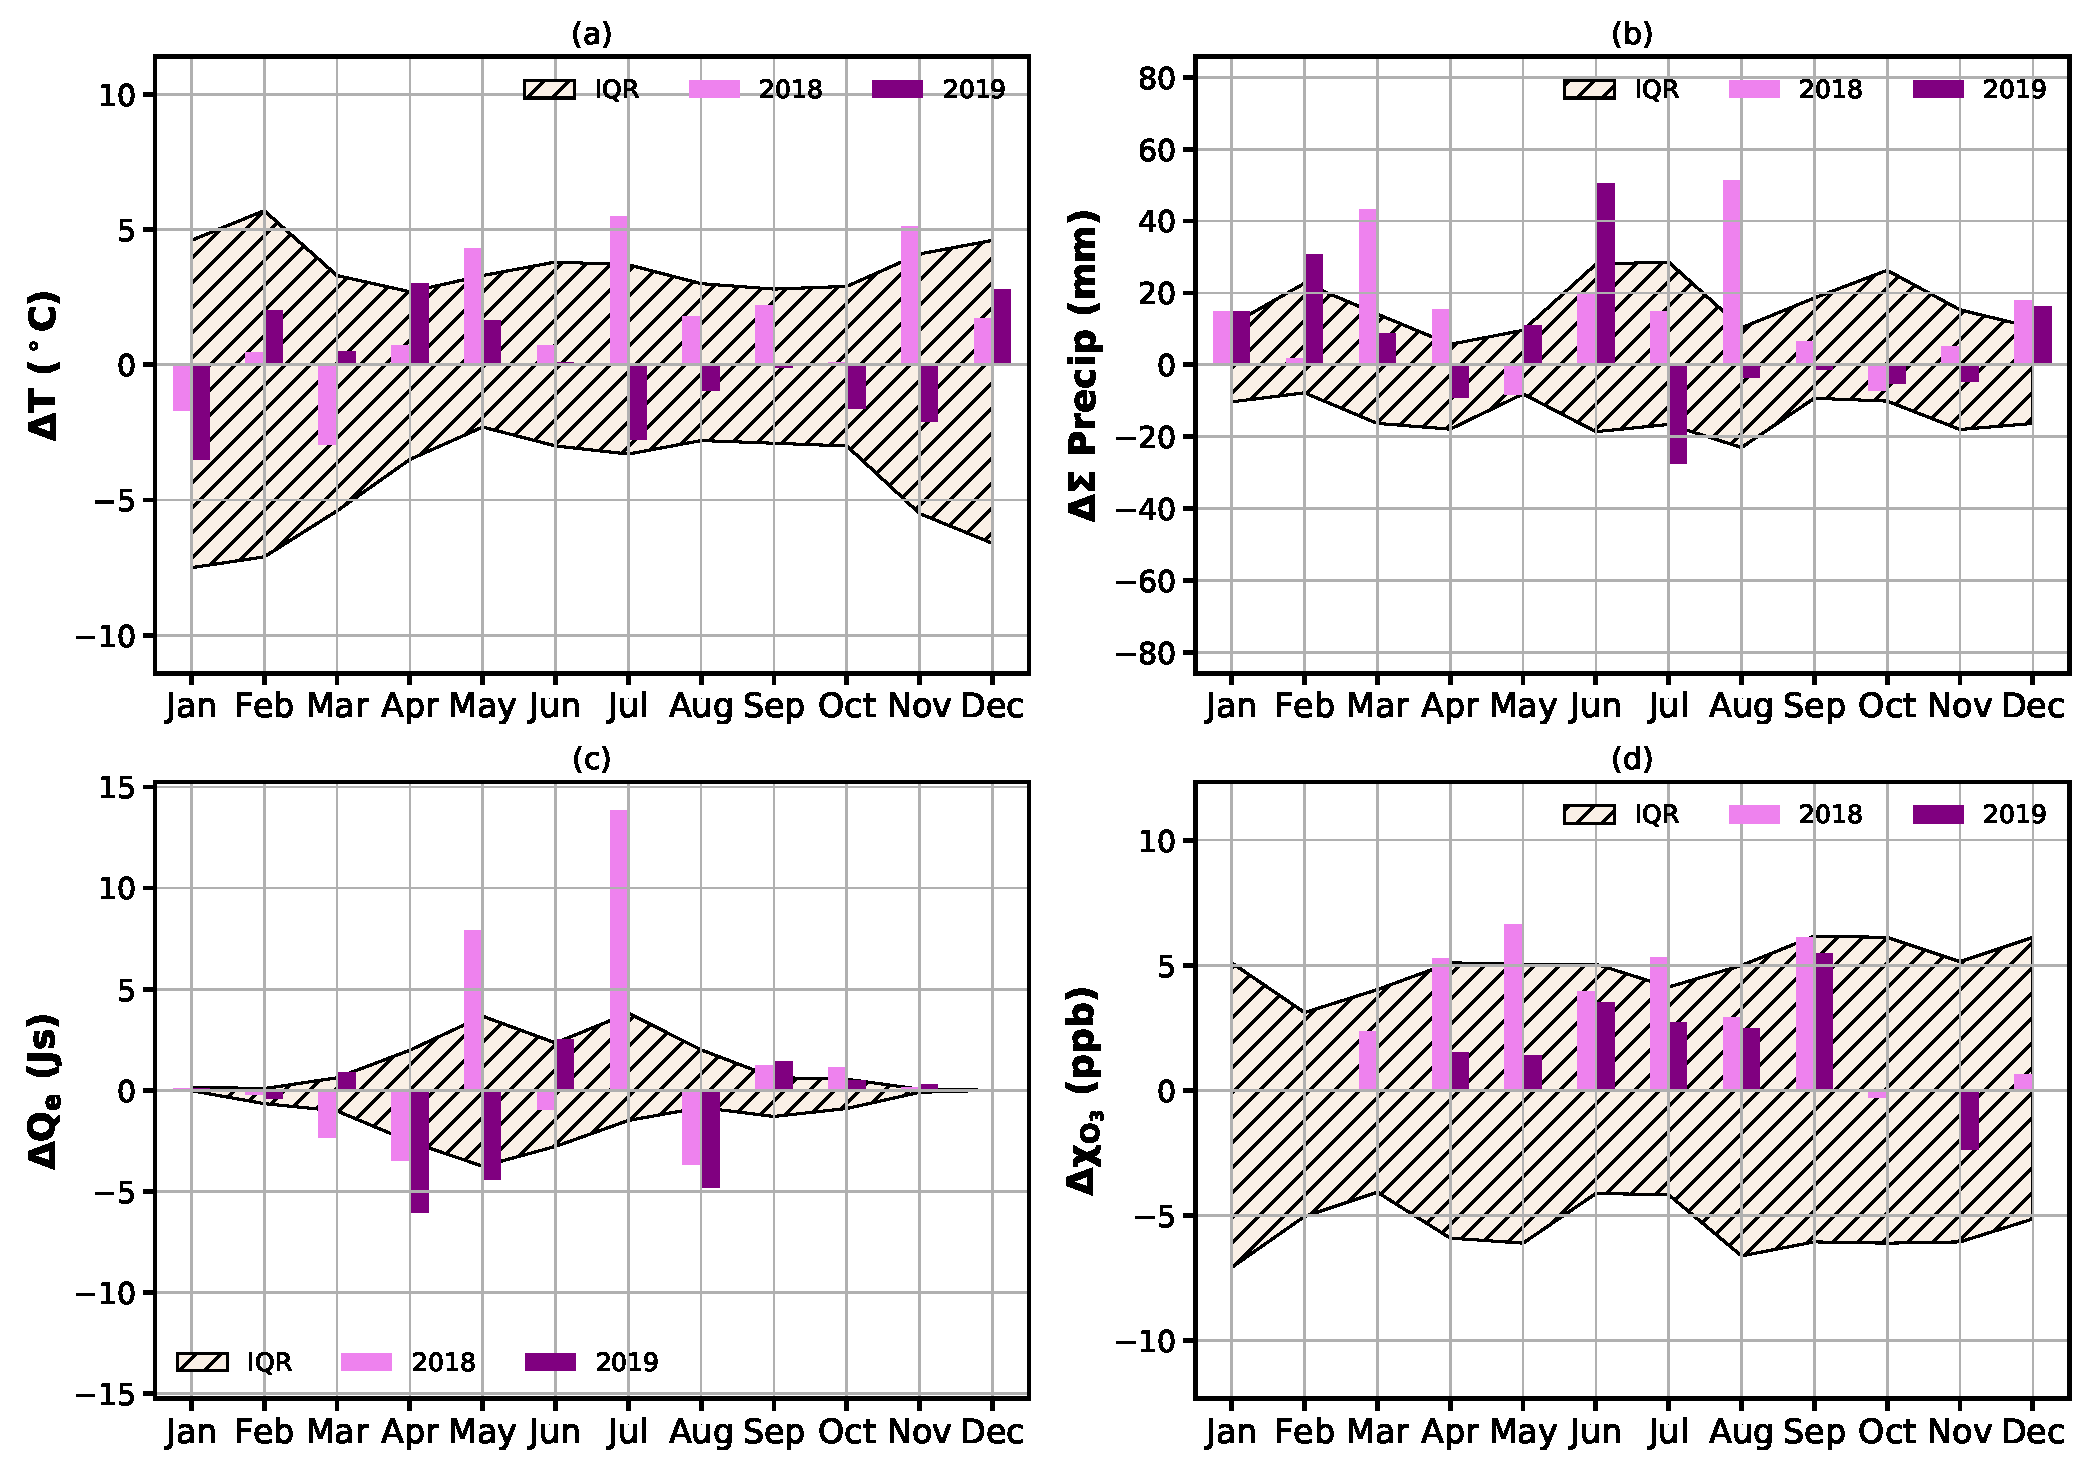
\includegraphics[width=12cm]{anomalies}
  \caption{2018/19 anomalies of key environmental variables at Svanhovd displayed as difference from median for each month. The hatched area between indicates the IQR. (a) Temperature; (b) precipitation; (c) radiant energy; (d) ozone VMR.}
  \label{fig:anomalies_svanvik}
\end{figure*}

\conclusions[Discussion and conclusions]
\label{sec:conc}

TODO: Compare with dry deposition velociteis from Finland.

For our study, we conducted a similar bio-monitoring study at Svanhovd, a site with agrometeorological and air pollution monitoring, to assess whether local ozone concentrations were capable of inducing damage to vegetation growing under northern Fennoscandia conditions. In 2018, we indeed observed ozone damage on clover and tobacco. In contrast, no such damage was found on the clovers in 2019. This indicates that key environmental variables in 2018 differed from 2019.

According to a report by the Norwegian Meteorological institute \citep{MetNOR2019}, the summer of 2018 was the warmest and driest ever recorded in eastern, western, and southern Norway. In the north (including Finnmark), it was amongst the warmest on record -- favorable conditions for ground-level ozone formation.
An unusually weak and northward shifted jet stream allowed for a persistent high-pressure system above northern Europe, including Fennoscandia which blocked the low-pressure systems for several consecutive months. In the period May -- July, southern Norway experienced temperatures $4\,\unit{^\circ C}$ above normal and saw only about $60\,\unit{\%}$ of normal precipitation. Northern Norway as a whole had close to normal precipitation, one of the causes of the high rate of forest fires in that area.
Thermal stress on vegetation was exceptional not only in large parts of Fennoscandia but also in much of Europe, where the influence of the high-pressure system extended even over five months (April/May, July--September). These conditions gave rise to massive forest fires in different parts of Europe and thus an increase in ozone precursors.
A total of 2079 forest fires were registered in Norway in 2018, twice as many as in the preceding years 2016/17 \citep{DSB2019}, last accessed April 2020). In Sweden, about 500 fires had been reported (five times more than in a usual summer), and an estimated total of $25000\,\unit{hectare}$ burned down in central Sweden (G\"{a}vleborgs, J\"{a}mtlands, and Dalarnas l\"{a}n) \citep{SOU2019}. Boreal wildfires are found to emit ozone precursors \chem{CO} ($\chem{[CO]}/\chem{[CO_2]} \propto 6-13\,\unit{\%}$) and VOCs ($\chem{[VOCs]}/\chem{[CO_2]} \propto 0.5-1.5\,\unit{\%}$) \citep{AE:Cofer1990}. Coincident peak \chem{\chi_{O_3}} is found in ozone monitoring data (Fig.~\ref{fig:data_svanvik_2018_2019}) in July. It is very likely that elevated ozone, like during the 2003 drought period \citep{JGR:Solberg2018}, was promoted by a combination of various factors such as wildfires, reduced cloud cover (increased solar radiation), reduced dry deposition and turbulent mixing due to the stagnant weather conditions, and increased BVOC emissions. As such events may become more frequent in the future, conditions at Svanhovd for the growing seasons 2018 shall serve as a reference for probable future conditions in northern Fennoscandia. Conditions in 2019 represent the present climate.\\


To summarize, we have developed bespoke parameterizations of common vegetation types (coniferous and deciduous trees, perennial grassland) to a subarctic climate and studied their effect on $\mathrm{POD_y}$. The comparison between meteorological conditions in 2018 and 2019 and their divergence from climatology allowed us to assess the influence of key environmental variables such as temperature, PPFD, and precipitation on vegetation susceptibility to \chem{O_3} damage in light of future changes as may occur under climate change. We found that conditions for ozone formation were more favorable in the 2018 growing season than in 2019, with 2018 being significantly warmer and less cloudy in spring and early summer. Accordingly, peak ozone concentrations occurred more frequently and at higher levels in 2018. This was particularly a result of the extended heatwave in spring and early summer and associated, extensive wildfires in Central Sweden. However, ozone concentrations during the growing season were not significantly enhanced and \chem{POD_1} values were very similar for both years.
This suggests that the overall length of the growing season is more crucial in risk assessment when using flux-based metrics than episodes of peak concentrations as these peak \chem{\chi_{O_3}} often coincide with environmental conditions that limit ozone uptake in the $\mathrm{DO_3SE}$ model.

Based on a MODIS photosynthesis product \citep{MODIS_PSN}, we estimated the growing season for coniferous trees in 2018 to be at least one month shorter than in 2019. The determined start of growing season in 2018 ($\unit{doy}~122$) and 2019 ($\unit{doy}~106$) lies within the range given by observations in Fennoscandia \citep{TB:Kolari2007,IVL:Karlsson2018}. We determined the start of the growing season for deciduous trees based on gridded observational temperature and for perennial grassland on snow depth data. For perennial grassland, we assumed an one-month latency period after snowmelt that is supported by observational data from Rovaniemi (Finland) \citep{FCR:Korhonen2018}. With respect to ongoing climate change, a clear positive trend emerged in length ($5.2\,\unit{d\,decade^{-1}}$) of the growing season that is almost equally distributed between earlier start ($2.9\,\unit{days\,decade^{-1}}$) and later end ($2.3\,\unit{d\,decade^{-1}}$) (Appendix Fig.~\ref{fig:greening_season_change_Svanvik}).

 The $\mathrm{DO_3SE}$ modeling results are in contrast to our observation of more visible damage in 2018 compared to 2019. However, visible damage caused by peak ozone uptake and dependence of ozone sensibility on phenology are not accounted for in $\mathrm{POD_y}$. In this regard, open-top chamber (OTC) experiments performed in northern Finland where Scots pine and downy birch seedlings were exposed to elevated ozone concentrations attributed a reduction in biomass and reproduction with visible damage explicitly to peak \chem{O_3} concentrations and fast phenological development at high growth rate \citep{Amb:Manninen2009}. In particular, forbs and perennial grassland are more susceptible to ozone-induced damage in the reproductive state \citep{EP:Bassin2004}. 
That might explain why we observed damage in the ozone garden to a larger extent in 2018 than in 2019. An associated damage function to ozone depending on leaf age as proposed by \citet{AE:Musselman2006} or phenological state might improve the predictions.

At the same time, intra-species variability even at the same location is typically non-negligible \citep{EP:Bassin2004} but not accounted for in the models. The literature results regarding the ozone sensitivity of natural vegetation in northern Europe are contradictive. \citet{FS:Subramanian2014} reported a higher, modeled reduction of net primary production in conifers ($4.3-15.5\,\unit{\%}$) than birch ($1.4-4.3\,\unit{\%}$) under elevated ozone in Sweden, while \citet{Amb:Girgzdiene2009} observed more visible damage on deciduous trees than on Norway spruce in Lithuania. But visible damage and biomass reduction may not occur at the same rate and hence may not be interchangeable. 

In our study, we do not explicitly account for this natural distribution of individual plant traits, but our bespoke response functions reflect the diversity within a given species. In particular, we assumed two tolerance levels to cold temperatures than for central European species. To this end, we computed a PDF from observed temperature at Svanhovd (May--September 1992--2000). We adjusted the parameters in the temperature response function of stomatal conductance to increase the enclosed area with the PDF. Assuming a proportionality between $g_\mathrm{sto}$ and $A_\mathrm{n}$, this is equivalent to optimizing carbon uptake. Similarly, we determined a PPFD PDF and varied the light response function to test a higher or lower extent of stomatal opening at low light intensities. Remark that these parameterizations are hypothetical and need verification by experimental data. We found that soil water potential under 2018/19 meteorological conditions was negligible when considering the bespoke growing season. We have not assessed the effect of the plants' response to VPD in detail, but our climatological data indicated that conditions at Svanhovd are shifting towards a more VPD limited regime. 

Our key findings are: 
\begin{enumerate}
\item Our bespoke parameterizations for subarctic species are better suited to describe vegetation adapted to subarctic conditions for instance allowing for stomata opening during a larger part of the growing season, 
\item the parameterizations defined in the mapping manual for European regional risk assessment appear to not adequately capture the physiological responses of subarctic vegetation that are important determinants of \chem{\chi_{O_3}} susceptibility and are likely to underestimate ozone-damage risk, and 
\item climatic conditions that are promoting a longer growing season are likely to increase the ozone-damage risk in flux-based metrics.
\end{enumerate}

In this regard, vegetation might become more exposed to higher ozone concentrations in early phenological stages due to an overlap with ozone spring peak \citep{EP:Karlsson2007}. However, the decline of this ozone spring peak is partly caused by the uptake of vegetation. It, therefore, remains unclear whether an earlier start of the growing season will increase the exposure of vegetation to ozone or lead to compensation due to an earlier decline of the peak ozone in the future. \citet{ESPR:Hayes2021} pointed out that the highest susceptibility of vegetation to future ozone variability is likely to occur in summer when vegetation is most productive. The actual resilience of northern Fennoscandia plant communities to climate change strongly depends on both the range of existing acclimations as well as the actual type of acclimation. This means vegetation that is acclimated to cold temperatures and little to heat- and drought stress might suffer more strongly from a more frequent occurence of heatwaves than plants that have a higher temperature tolerance.

Following the methods described in \citet{ICP:MappingManual2017}, we estimated biomass reductions due to ozone uptake for both 2018 and 2019 and found substantial reductions for deciduous trees ($15.5-17.4\,\unit{\%}$) and perennial grassland (above ground, $12.4-13.7\,\unit{\%}$) in both years. These reductions are higher than for the default parameterizations, $11.2\,\unit{\%}$ (deciduous) and $9.6\,\unit{\%}$ (perennial grassland). For coniferous trees, the estimated reduction in biomass differs insignificantly between our bespoke parameterizations ($2.5-3\,\unit{\%}$) and the default ($2.31\,\unit{\%}$). This indicates a higher modeled robustness to ozone damage in coniferous trees. All these results have to be treated with care because the biomass reduction functions were established based on studies from less extreme climates. In particular, CLs for deciduous and coniferous trees were breached in all years and for all parameterizations. For perennial grassland, the CL was not breached if a bespoke GS was assumed, but the mapping manual defined CL of $10\,\unit{\%}$ loss in biomass might not be transferable to subarctic regions with considerable constraints on productivity leading to more severe economical consequences.

Beyond the risk assessment of ozone-induced damage, our bespoke temperature response functions, once verified by observations, can have important implications on land-surface modeling in global models, where problems in productivity of species especially in the Arctic regions occur due to PFTs which are not suitable for the climate. We pointed out, concerning default perennial grassland parameterization, that these perennial grasslands did not show any substantial stomatal conductance in 2019 characterized as a normal year. In terms of GPP this would mean unrealistically low carbon uptake. Automation of the here proposed PDF-based acclimation using machine learning techniques could overcome these issues in the future.

%% The following commands are for the statements about the availability of data sets and/or software code corresponding to the manuscript.
%% It is strongly recommended to make use of these sections in case data sets and/or software code have been part of your research the article is based on.

%\codeavailability{TEXT} %% use this section when having only software code available


\dataavailability{All data is available from public databases or through institutional access. $\mathrm{DO_3SE}$ modeling results can be made available upon request.} %% use this section when having only data sets available


%\codedataavailability{TEXT} %% use this section when having data sets and software code available


%\sampleavailability{TEXT} %% use this section when having geoscientific samples available


%\videosupplement{TEXT} %% use this section when having video supplements available
\clearpage

\appendix
\section{Growing season}
\label{appendix:growing_season}

\begin{figure*}[th]
  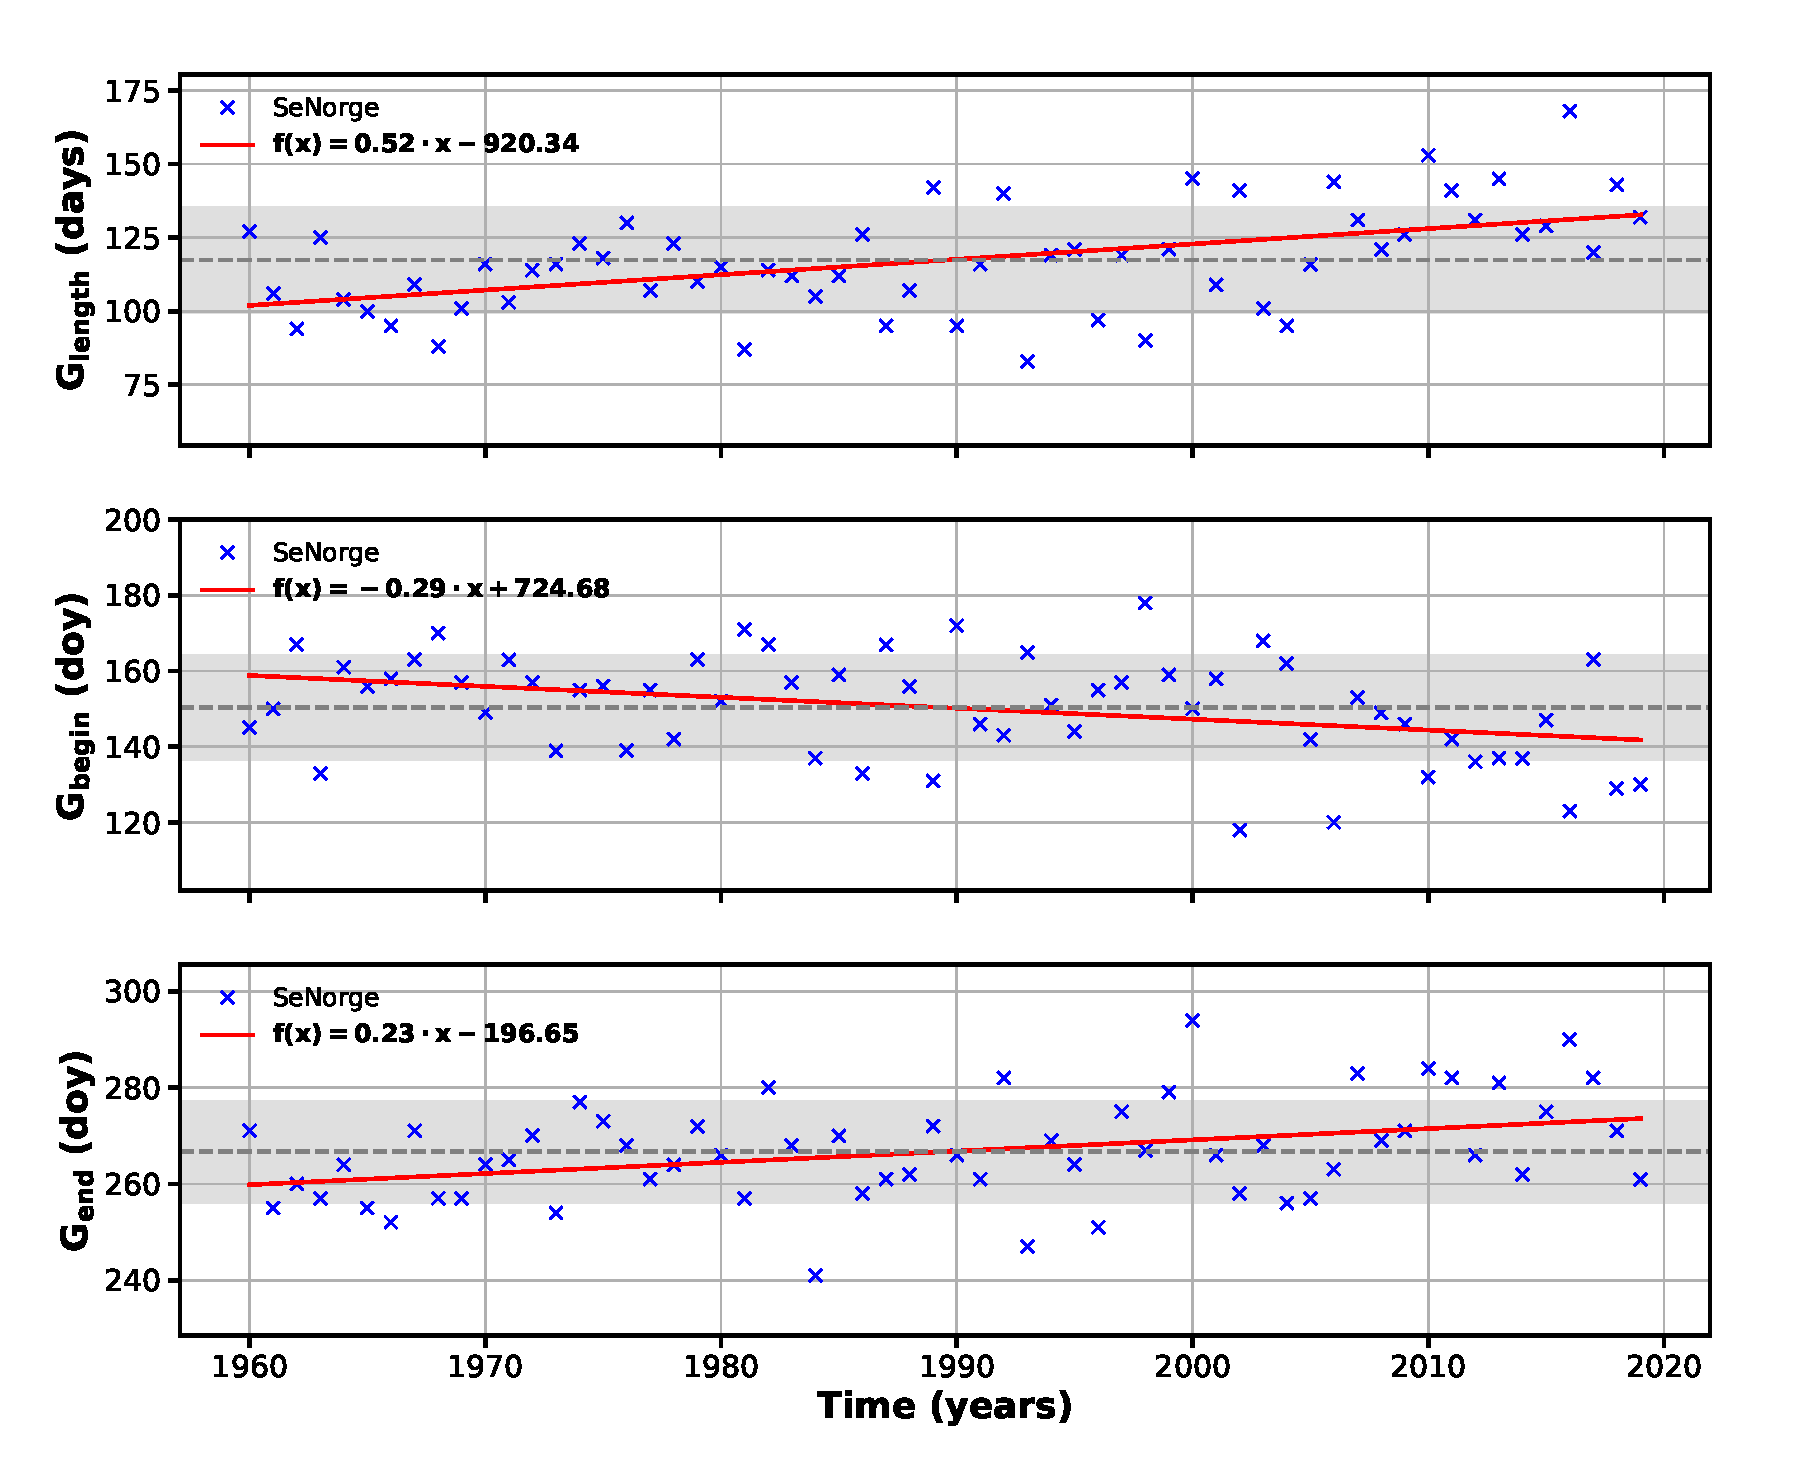
\includegraphics[width=12cm]{greening_season_change_Svanvik}
  \caption{Estimated shift and prolongation of growing season at Svanhovd over the past 6 decades based on data from \citet{SeNorge}.}
  \label{fig:greening_season_change_Svanvik}
\end{figure*}

\section{DO3SE model}
\label{appendix:do3se_model}


\subsection{Initial $\mathrm{DO_3SE}$ modeling results with mapping manual parameters}
To demonstrate the necessary acclimation of the mapping manual parameters, we show the initial results of stomatal conductance at leaf-level ($G_\mathrm{sto}^\mathrm{leaf}$) and $\mathrm{POD_y}$ over \unit{doy} for both years and all PFTs (Fig.~\ref{fig:pody_mm_composit}). Observed \chem{\chi_{O_3}} is also indicated. From Fig.~\ref{fig:pody_mm_composit}f) it is apparent that the mapping manual parameterized grassland would not have been able to grow in 2019.

\begin{figure*}[t]
  %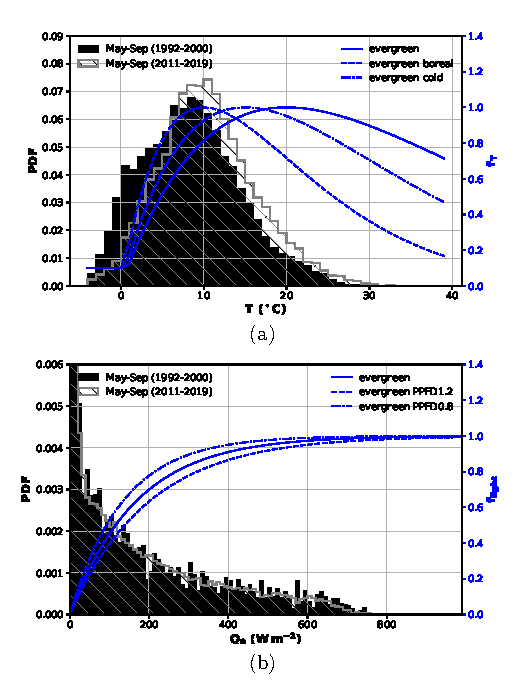
\includegraphics[width=12cm]{figB1}
  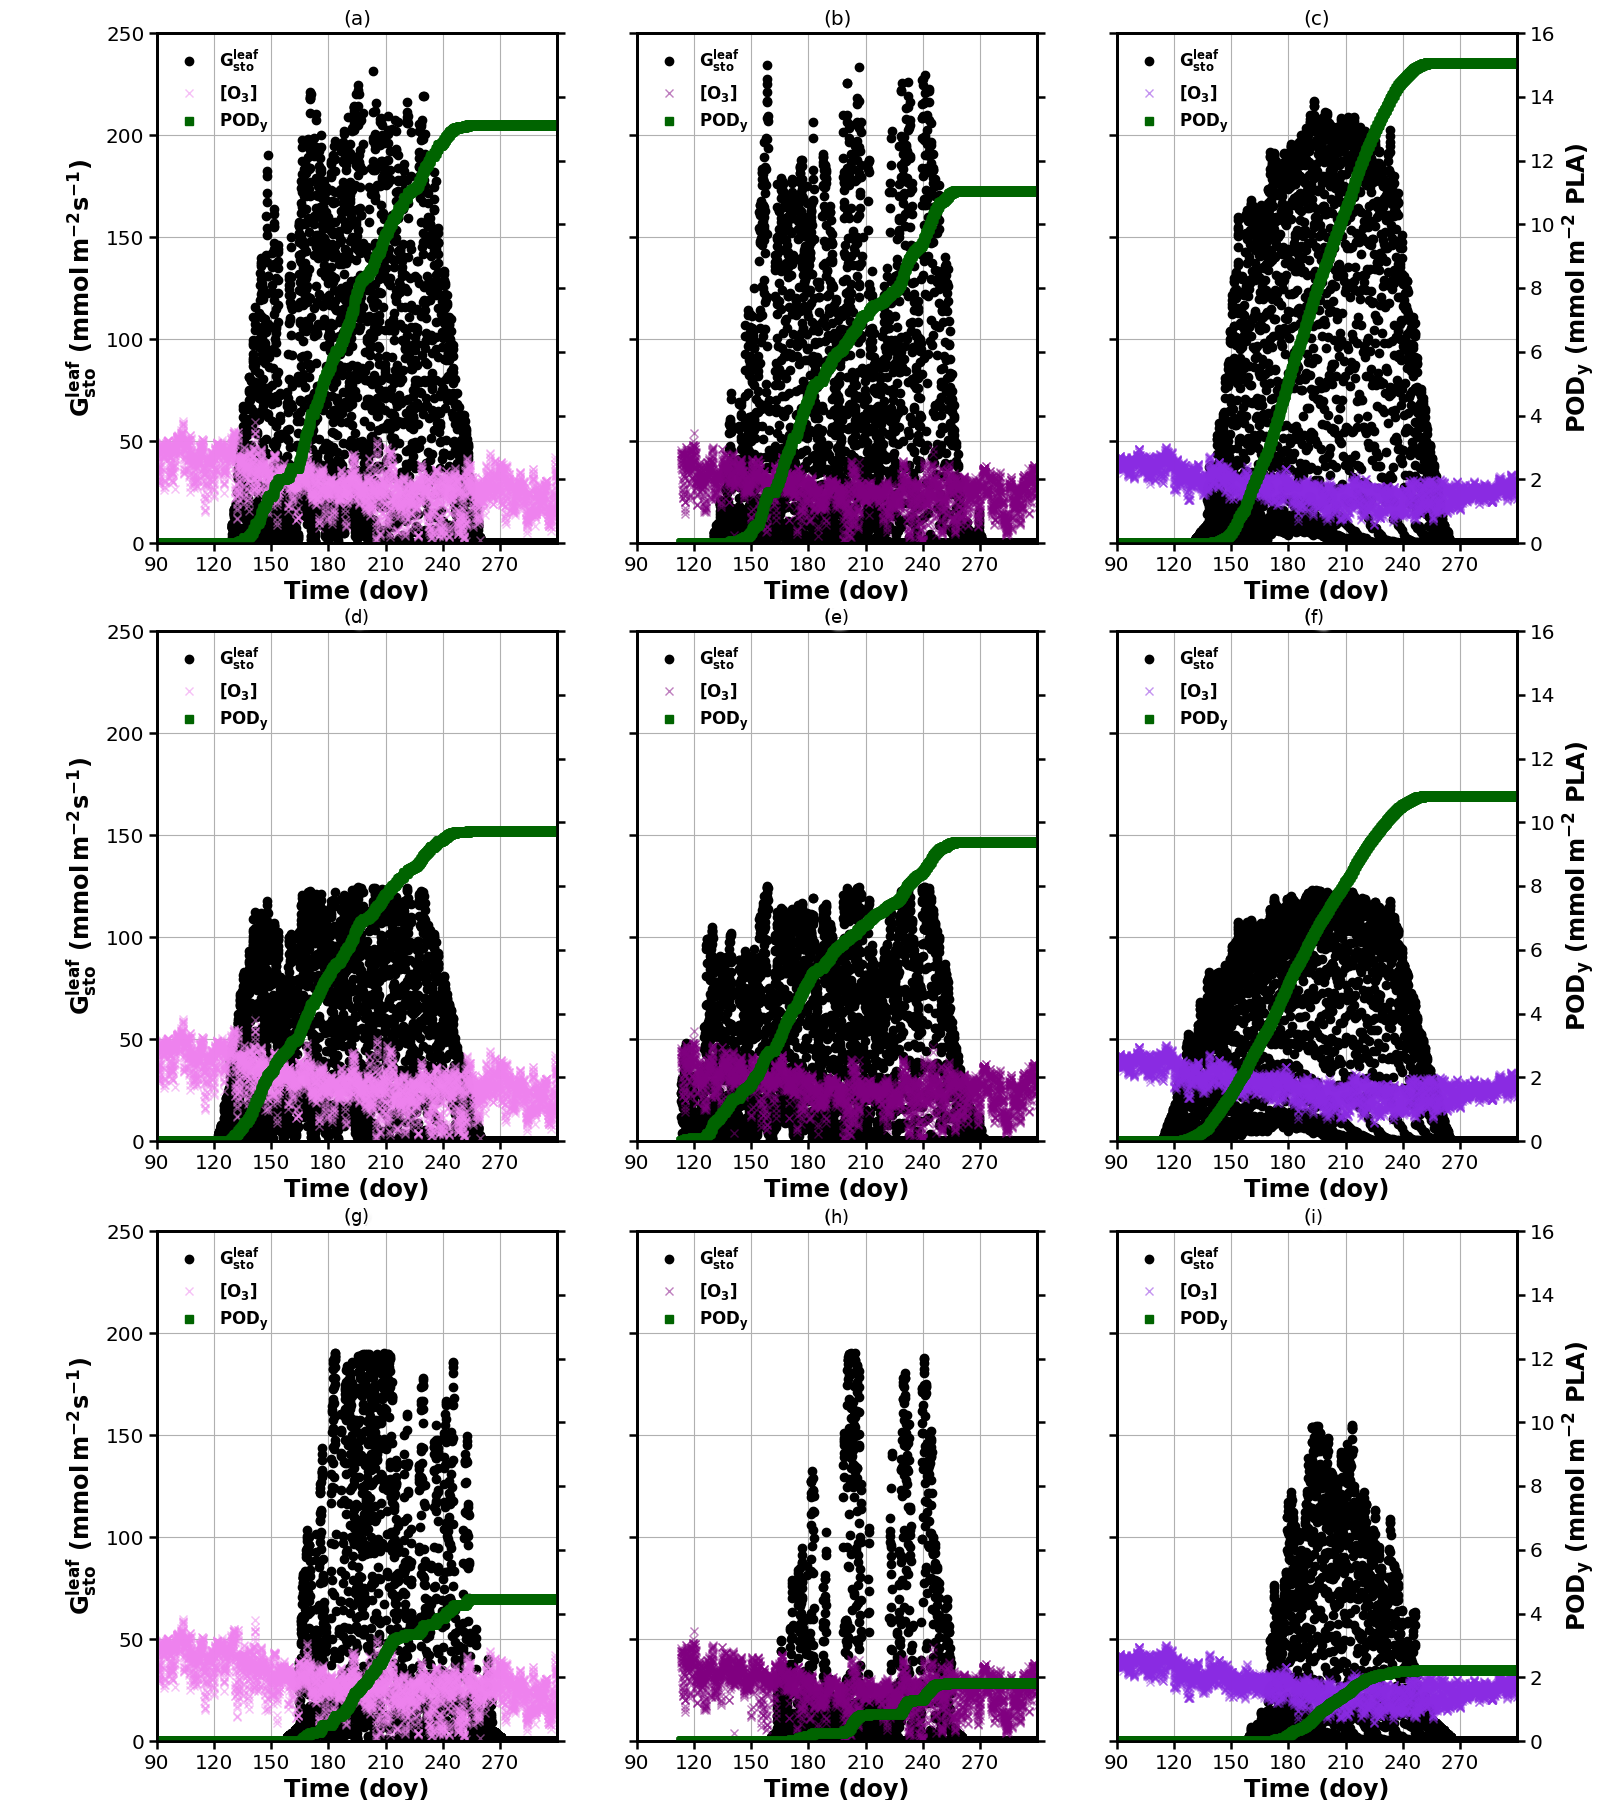
\includegraphics[width=12cm]{DO3SE_results_pody_gsto_o3.png}
  \caption{$\mathrm{DO_3SE}$ modeling results for mapping manual default parameterization. $\mathrm{POD_y}$ is shown over \unit{doy}, March--October. A flux threshold $y=1\,\unit{nmol\,m^{-2}\,s^{-1}}$ per projected leaf area (PLA) has been chosen. \chem{\chi_{O_3}} are plotted on the same axis and scales as $G_\text{sto}^\text{leaf}$ but in units of $\unit{ppb}$. (a, b) deciduous tree; (c, d) coniferous tree; (e, f) perennial grassland. From left to right: 2018, 2019.}
  \label{fig:pody_mm_composit}
\end{figure*}

\subsection{Bespoke parameterizations}

To assess the $G_\mathrm{start}$  and $G_\mathrm{end}$ of the growing season for coniferous trees at Svanhovd in 2018/19, we used the net photosynthesis product ($A_\mathrm{net}$) of MODIS AQUA/TERRA over a $1\times 1\,\unit{km}$ area centered at Svanhovd. MODIS data indicate a higher photosynthetic activity in 2018 than in 2019. As shown in Fig.~\ref{fig:modis_gpp} we fitted a second order polynomial function of the general form
%
\begin{equation}
A_\mathrm{net}(t) =  -m_0\cdot(t-m_1)^2+m_2,
\end{equation}
%
with the form parameters $m_i$ through the data. Numerically, we retrieved the roots as $G_\mathrm{start}$ 122/106 and $G_\mathrm{end}$ 261/274 for 2018 and 2019, respectively. 

\begin{figure}[th]
  %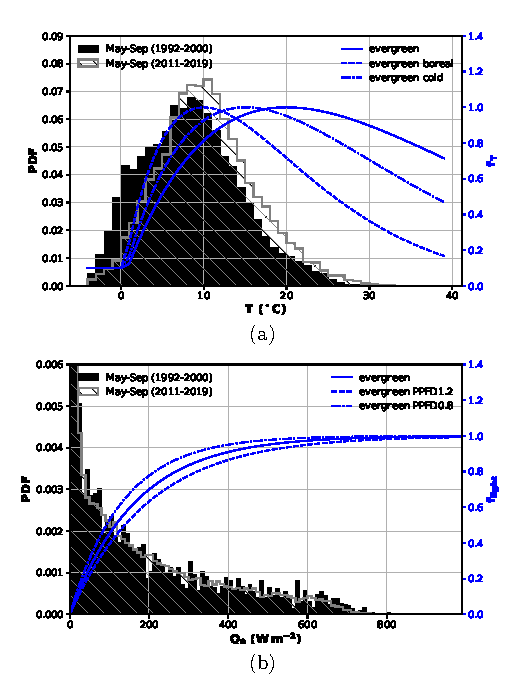
\includegraphics[width=8.3cm]{figB2}
  \includegraphics[width=8.3cm]{modis_gpp}
  \caption{Estimated $G_\mathrm{start}$ and $G_\mathrm{end}$ of growing season for coniferous trees from MODIS Aqua/Terra gross primary productivity (GPP) product. A $1\times 1\,\unit{km}$ area around Svanhovd was selected. Daily averaged data for both 2018 and 2019 has been fitted with a quadratic polynomial function. The numerically computed root yields: BGS \unit{doy}~122/106 and EGS \unit{doy}~261/274 for 2018/19, respectively.}
  \label{fig:modis_gpp}
\end{figure}

As described in Section~\ref{subsec:do3se_parameters}, we developed bespoke parameterizations for natural and semi-natural vegetation at Svanhovd. Here, we show the temperature response and light response functions for coniferous and deciduous trees (Figs.~\ref{fig:f_temp_spruce}-\ref{fig:f_temp_birch}). 

\begin{figure}[t]
  \centering
  (a)\\
  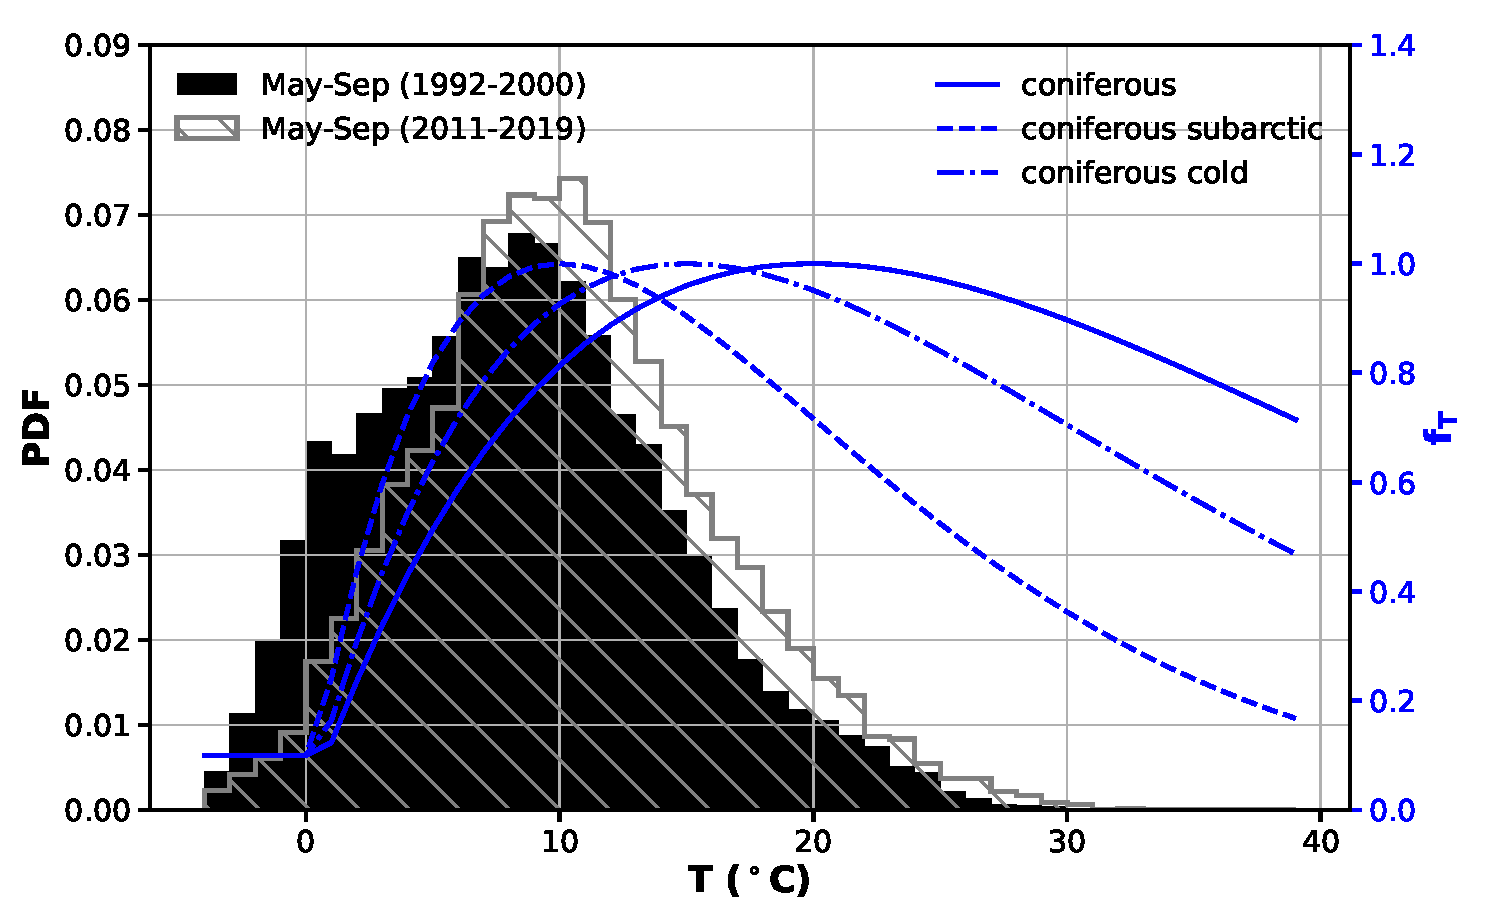
\includegraphics[width=8.3cm]{javis_funcs_temp_hist_coniferous}\\
  (b)\\
  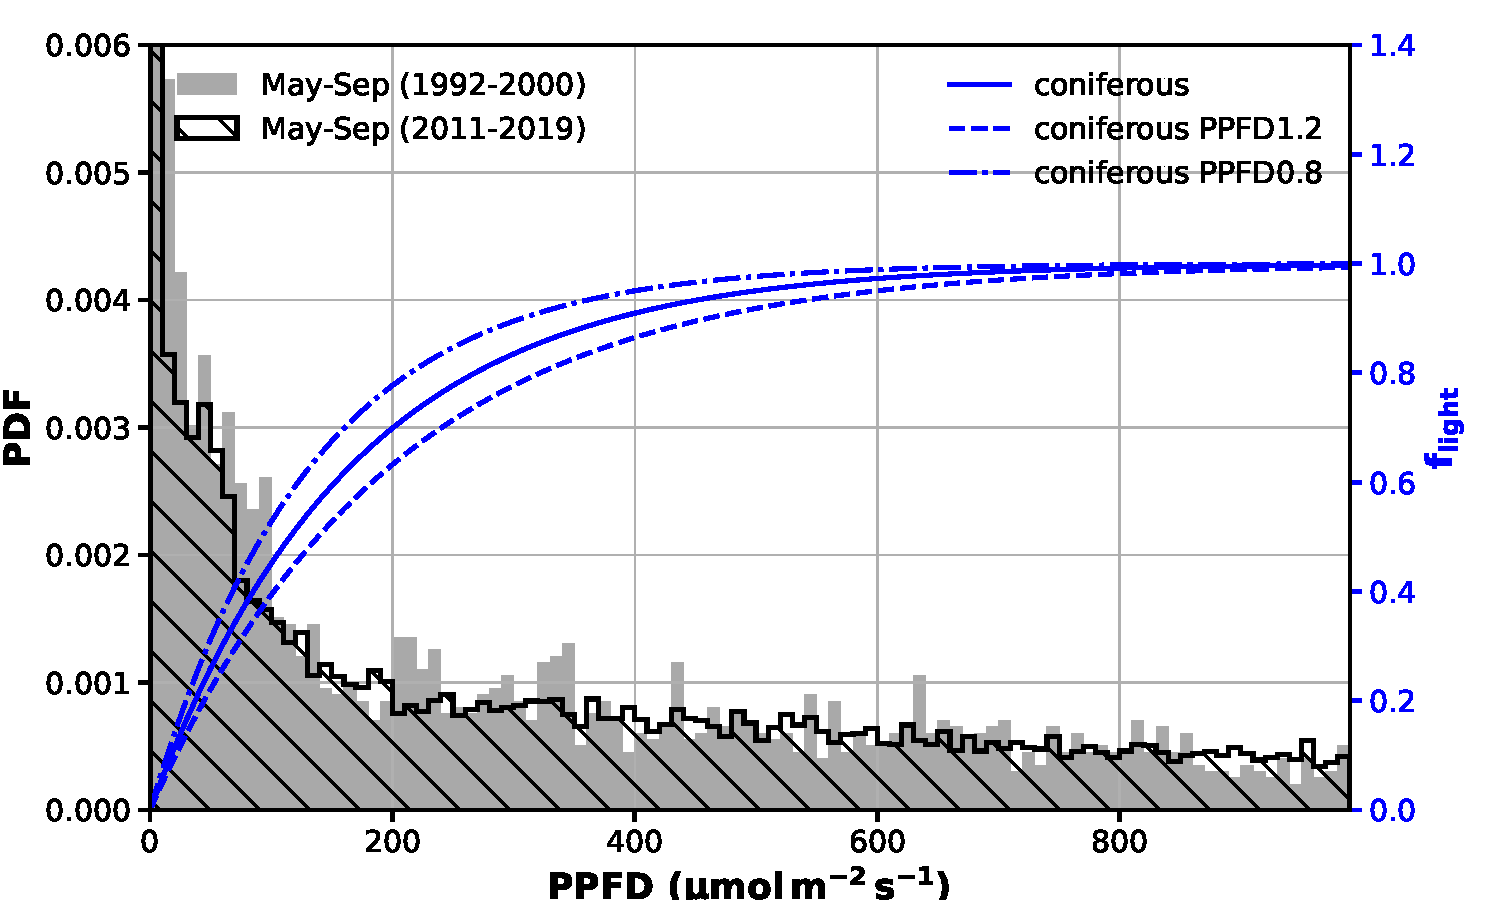
\includegraphics[width=8.3cm]{javis_funcs_light_hist_coniferous.pdf}
  %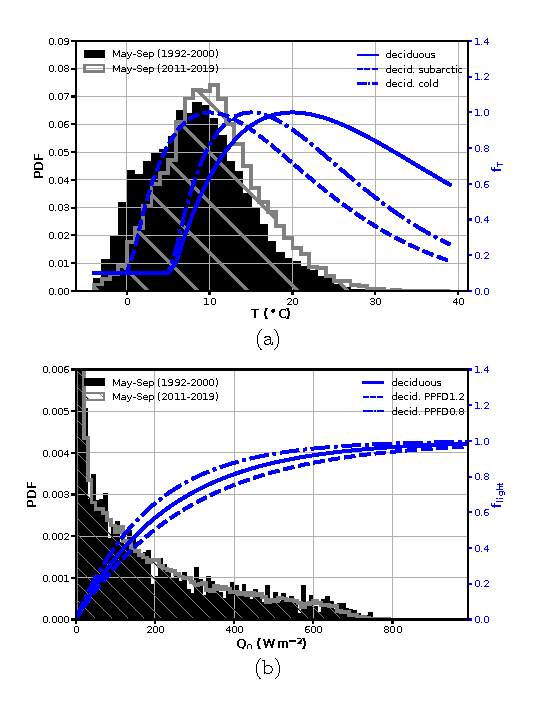
\includegraphics[width=8.3cm]{figB3}
\caption{Construction of bespoke response functions for coniferous trees. (a) $f_\mathrm{T}$ and (b) $f_\mathrm{flight}$ are shown together with underlying $T_\mathrm{air}$ and $Q_0$ climatologies (probability density function - PDF), respectively. Original mapping manual parameterization is shown in comparison as solid line. Note that $Q_0$ has been truncated to $0.006$. PPFD0.8 and PPFD1.2 refer to $\alpha$ values increasing/decreasing PPFD at $f_\mathrm{light}=0.5$ by $\pm 20\,\%$, respectively.}
\label{fig:f_temp_spruce}
\end{figure}

\begin{figure}[t]
  \centering
  (a)\\
  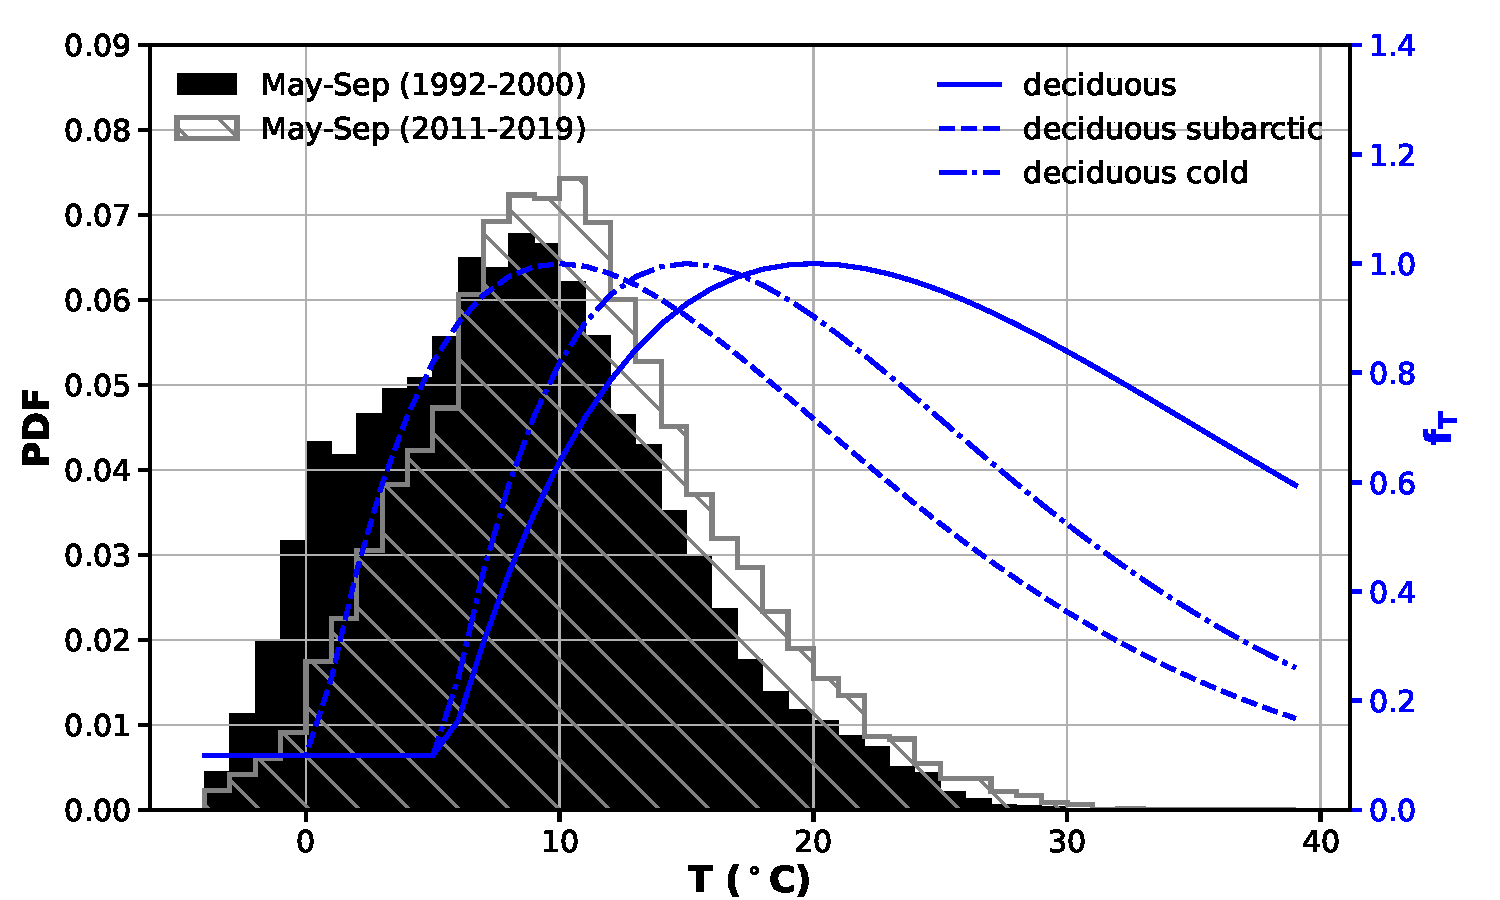
\includegraphics[width=8.3cm]{javis_funcs_temp_hist_deciduous.pdf}\\
  (b)\\
  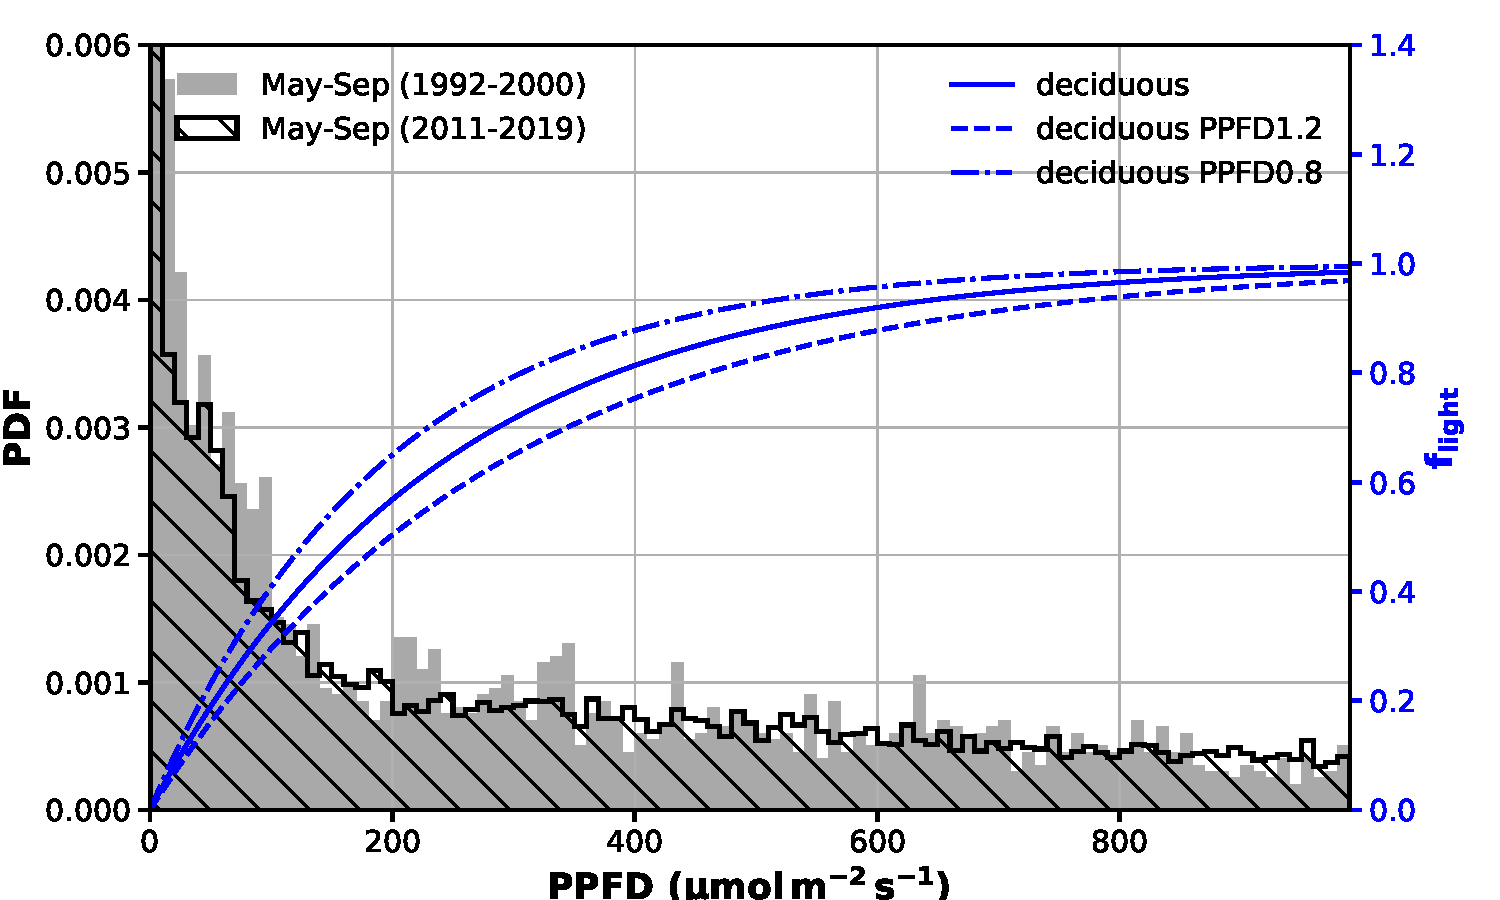
\includegraphics[width=8.3cm]{javis_funcs_light_hist_deciduous.pdf}
  %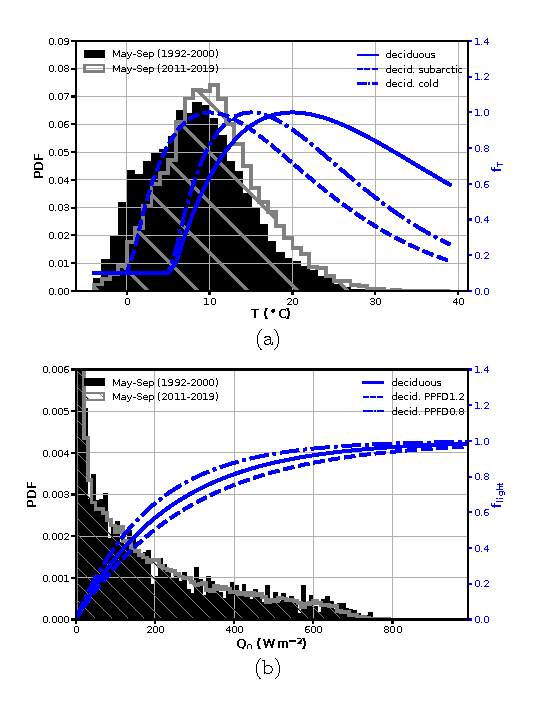
\includegraphics[width=8.3cm]{figB4}
\caption{Construction of bespoke response functions for deciduous trees. (a) $f_\mathrm{T}$ and (b) $f_\mathrm{flight}$ are shown together with underlying $T_\mathrm{air}$ and $Q_0$ climatologies (probability density function - PDF), respectively. Original mapping manual parameterization is shown in comparison as solid line. Note that $Q_0$ has been truncated to $0.006$. PPFD0.8 and PPFD1.2 refer to $\alpha$ values increasing/decreasing PPFD at $f_\mathrm{light}=0.5$ by $\pm 20\,\%$, respectively.}
\label{fig:f_temp_birch}
\end{figure}

\clearpage

\noappendix       %% use this to mark the end of the appendix section. Otherwise the figures might be numbered incorrectly (e.g. 10 instead of 1).

%% Regarding figures and tables in appendices, the following two options are possible depending on your general handling of figures and tables in the manuscript environment:

%% Option 1: If you sorted all figures and tables into the sections of the text, please also sort the appendix figures and appendix tables into the respective appendix sections.
%% They will be correctly named automatically.

%% Option 2: If you put all figures after the reference list, please insert appendix tables and figures after the normal tables and figures.
%% To rename them correctly to A1, A2, etc., please add the following commands in front of them:

%\appendixfigures  %% needs to be added in front of appendix figures


%\noappendix

%\appendixtables   %% needs to be added in front of appendix tables

%% Please add \clearpage between each table and/or figure. Further guidelines on figures and tables can be found below.



\authorcontribution{All authors contributed to conceptualization of this research article and commented on the manuscript. SF has prepared the original draft, collected and processed ozone and environmental data, and performed all statistical analyses. AVV has conducted the on-site observation of vegetation damage induced by ozone, provided advice on plant physiological processes, collected existing literature on subarctic vegetation, contributed significantly proofreading this research article. LE has contributed with expertise in $\mathrm{DO_3SE}$ modeling and suggestion of the PDF-based temperature acclimation methodology. CO has collected PFT parameters from the literature, performed all $\mathrm{DO_3SE}$ simulations and validation. AE contributed with her experience regarding subarctic vegetation in Finnmark. FS contributed with an assessment of the 2018 meteorological conditions. TB gave valuable guidance in a broader research sense. Funding acquisition for the project: AVV, AE, FS, TB.} %% this section is mandatory

\competinginterests{The authors declare that they have no conflict of interest.} %% this section is mandatory even if you declare that no competing interests are present

%\disclaimer{TEXT} %% optional section

\begin{acknowledgements}
  We thank NILU for performing the ozone measurements at Svanhovd for us, Bj{\o}rg Rognerud (Department of Geosciences, UiO) for processing SeNorge.no data with respect to the beginning of the growing season, Tore Flatlandsmo Berglen (NILU) for hourly pressure data from Svanhovd, NIBIO Environment Center Svanhovd for establishing and running the ozone garden both years, and Volkmar Timmermann (NIBIO) for sharing ICP Forest data from Svanhovd. This work was supported by the Research Council of Norway (Grant No. 268073).
\end{acknowledgements}




%% REFERENCES

%% The reference list is compiled as follows:

%\begin{thebibliography}{}

%\bibitem[AUTHOR(YEAR)]{LABEL1}
%REFERENCE 1

%\bibitem[AUTHOR(YEAR)]{LABEL2}
%REFERENCE 2

%\end{thebibliography}

%% Since the Copernicus LaTeX package includes the BibTeX style file copernicus.bst,
%% authors experienced with BibTeX only have to include the following two lines:
%%
\bibliographystyle{copernicus}
\bibliography{atmo.bib}
%%
%% URLs and DOIs can be entered in your BibTeX file as:
%%
%% URL = {http://www.xyz.org/~jones/idx_g.htm}
%% DOI = {10.5194/xyz}


%% LITERATURE CITATIONS
%%
%% command                        & example result
%% \citet{jones90}|               & Jones et al. (1990)
%% \citep{jones90}|               & (Jones et al., 1990)
%% \citep{jones90,jones93}|       & (Jones et al., 1990, 1993)
%% \citep[p.~32]{jones90}|        & (Jones et al., 1990, p.~32)
%% \citep[e.g.,][]{jones90}|      & (e.g., Jones et al., 1990)
%% \citep[e.g.,][p.~32]{jones90}| & (e.g., Jones et al., 1990, p.~32)
%% \citeauthor{jones90}|          & Jones et al.
%% \citeyear{jones90}|            & 1990



%% LITERATURE CITATIONS
%%
%% command                        & example result
%% \citet{jones90}|               & Jones et al. (1990)
%% \citep{jones90}|               & (Jones et al., 1990)
%% \citep{jones90,jones93}|       & (Jones et al., 1990, 1993)
%% \citep[p.~32]{jones90}|        & (Jones et al., 1990, p.~32)
%% \citep[e.g.,][]{jones90}|      & (e.g., Jones et al., 1990)
%% \citep[e.g.,][p.~32]{jones90}| & (e.g., Jones et al., 1990, p.~32)
%% \citeauthor{jones90}|          & Jones et al.
%% \citeyear{jones90}|            & 1990



%% FIGURES

%% When figures and tables are placed at the end of the MS (article in one-column style), please add \clearpage
%% between bibliography and first table and/or figure as well as between each table and/or figure.

% The figure files should be labelled correctly with Arabic numerals (e.g. fig01.jpg, fig02.png).


%% ONE-COLUMN FIGURES

%%f
%\begin{figure}[t]
%\includegraphics[width=8.3cm]{FILE NAME}
%\caption{TEXT}
%\end{figure}
%
%%% TWO-COLUMN FIGURES
%
%%f
%\begin{figure*}[t]
%\includegraphics[width=12cm]{FILE NAME}
%\caption{TEXT}
%\end{figure*}
%
%
%%% TABLES
%%%
%%% The different columns must be seperated with a & command and should
%%% end with \\ to identify the column brake.
%
%%% ONE-COLUMN TABLE
%
%%t
%\begin{table}[t]
%\caption{TEXT}
%\begin{tabular}{column = lcr}
%\tophline
%
%\middlehline
%
%\bottomhline
%\end{tabular}
%\belowtable{} % Table Footnotes
%\end{table}
%
%%% TWO-COLUMN TABLE
%
%%t
%\begin{table*}[t]
%\caption{TEXT}
%\begin{tabular}{column = lcr}
%\tophline
%
%\middlehline
%
%\bottomhline
%\end{tabular}
%\belowtable{} % Table Footnotes
%\end{table*}
%
%%% LANDSCAPE TABLE
%
%%t
%\begin{sidewaystable*}[t]
%\caption{TEXT}
%\begin{tabular}{column = lcr}
%\tophline
%
%\middlehline
%
%\bottomhline
%\end{tabular}
%\belowtable{} % Table Footnotes
%\end{sidewaystable*}
%
%
%%% MATHEMATICAL EXPRESSIONS
%
%%% All papers typeset by Copernicus Publications follow the math typesetting regulations
%%% given by the IUPAC Green Book (IUPAC: Quantities, Units and Symbols in Physical Chemistry,
%%% 2nd Edn., Blackwell Science, available at: http://old.iupac.org/publications/books/gbook/green_book_2ed.pdf, 1993).
%%%
%%% Physical quantities/variables are typeset in italic font (t for time, T for Temperature)
%%% Indices which are not defined are typeset in italic font (x, y, z, a, b, c)
%%% Items/objects which are defined are typeset in roman font (Car A, Car B)
%%% Descriptions/specifications which are defined by itself are typeset in roman font (abs, rel, ref, tot, net, ice)
%%% Abbreviations from 2 letters are typeset in roman font (RH, LAI)
%%% Vectors are identified in bold italic font using \vec{x}
%%% Matrices are identified in bold roman font
%%% Multiplication signs are typeset using the LaTeX commands \times (for vector products, grids, and exponential notations) or \cdot
%%% The character * should not be applied as mutliplication sign
%
%
%%% EQUATIONS
%
%%% Single-row equation
%
%\begin{equation}
%
%\end{equation}
%
%%% Multiline equation
%
%\begin{align}
%& 3 + 5 = 8\\
%& 3 + 5 = 8\\
%& 3 + 5 = 8
%\end{align}
%
%
%%% MATRICES
%
%\begin{matrix}
%x & y & z\\
%x & y & z\\
%x & y & z\\
%\end{matrix}
%
%
%%% ALGORITHM
%
%\begin{algorithm}
%\caption{...}
%\label{a1}
%\begin{algorithmic}
%...
%\end{algorithmic}
%\end{algorithm}
%
%
%%% CHEMICAL FORMULAS AND REACTIONS
%
%%% For formulas embedded in the text, please use \chem{}
%
%%% The reaction environment creates labels including the letter R, i.e. (R1), (R2), etc.
%
%\begin{reaction}
%%% \rightarrow should be used for normal (one-way) chemical reactions
%%% \rightleftharpoons should be used for equilibria
%%% \leftrightarrow should be used for resonance structures
%\end{reaction}
%
%
%%% PHYSICAL UNITS
%%%
%%% Please use \unit{} and apply the exponential notation

\end{document}
